% !TeX root = ../MQF_Manuale_Master.tex
% Capitoli/MQF_Cap_09_Markov_Misure_Rischio.tex

\chapter{Catene di Markov e misure di rischio}

\label{cap:markov-misure-rischio}

\section{Obiettivi della lezione e problema guida}

\label{sec:cap9-obiettivi}

Nel Capitolo~8 la dinamica di un sistema economico o finanziario \`{e}
stata rappresentata mediante una catena di Markov finita. Assegnata una
matrice di transizione $P$, le sue potenze determinano le
probabilit\`{a} degli stati futuri:

\[
p_{ij}^{(h)}
=
\Prob(X_h=j\mid X_0=i)
=
(P^h)_{ij}.
\]

Se lo stato iniziale non \`{e} noto con certezza ed \`{e} descritto
dalla distribuzione $\pi_0$, la distribuzione degli stati
all'orizzonte $h$ \`{e}

\[
\pi_h=\pi_0P^h.
\]

Nel caso delle migrazioni del rating, questi risultati permettono di
determinare la probabilit\`{a} che un emittente migliori il proprio
merito creditizio, rimanga nella classe corrente, subisca un
deterioramento oppure entri nello stato assorbente di default.

La distribuzione degli stati futuri non coincide tuttavia con una
distribuzione delle perdite. La matrice di transizione descrive
\emph{quali stati possono verificarsi e con quale probabilit\`{a}}, ma
non stabilisce automaticamente quali conseguenze economiche derivino
da ciascuno stato.

Per mettere in evidenza questa distinzione, consideriamo due esposizioni
creditizie $A$ e $B$, aventi lo stesso nozionale, la stessa
scadenza e il medesimo tasso di recupero. Supponiamo inoltre che le due
esposizioni presentino la stessa probabilit\`{a} annuale di default,
pari al $3\%$, ma differenti probabilit\`{a} di migrazione:

\[
\begin{array}{lcccc}
\hline
&
\text{miglioramento}
&
\text{rating invariato}
&
\text{downgrade}
&
\text{default}
\\
\hline
\text{Esposizione }A
&
0.04
&
0.78
&
0.15
&
0.03
\\
\text{Esposizione }B
&
0.08
&
0.87
&
0.02
&
0.03
\\
\hline
\end{array}
\]

Se si osservasse soltanto la probabilit\`{a} di default, le due
esposizioni potrebbero apparire equivalenti. L'esposizione $A$
presenta per\`{o} una probabilit\`{a} di downgrade molto pi\`{u}
elevata. Se il deterioramento del rating determina un aumento del
credit spread e una riduzione del valore di mercato dello strumento,
la distribuzione delle perdite di $A$ pu\`{o} risultare sensibilmente
diversa da quella di $B$, anche se la probabilit\`{a} di default
\`{e} identica.

L'esempio mostra che la probabilit\`{a} di default costituisce una
componente essenziale del rischio di credito, ma non ne fornisce una
misura completa. Per passare dalle probabilit\`{a} alle perdite occorre
specificare almeno:

\begin{itemize}

\item l'esposizione economica soggetta a rischio;

\item la perdita subita in caso di default;

\item il valore recuperabile dopo il default;

\item la variazione di valore prodotta dalle migrazioni verso rating
migliori o peggiori;

\item l'orizzonte temporale sul quale il rischio viene misurato.

\end{itemize}

Il problema guida del capitolo \`{e} pertanto il seguente:

\begin{quote}
\emph{Come possiamo utilizzare le probabilit\`{a} di migrazione e di
default generate da una catena di Markov per costruire una
distribuzione monetaria delle perdite, misurare il rischio della sua
coda e valutare l'effetto di uno strumento di copertura come il credit
default swap?}
\end{quote}

Il percorso concettuale della lezione pu\`{o} essere rappresentato
mediante la sequenza

\[
P^h
\longrightarrow
\text{default e sopravvivenza}
\longrightarrow
L_h
\longrightarrow
\VaR_{\alpha}(L_h)
\longrightarrow
\CVaR_{\alpha}(L_h)
\longrightarrow
\text{CDS}.
\]

La matrice $P^h$ determina le probabilit\`{a} dei rating futuri e,
in particolare, la struttura temporale delle probabilit\`{a} di
default e di sopravvivenza. Associando a ciascuno stato futuro un
valore economico o una perdita si costruisce la variabile casuale
$L_h$. La sua distribuzione permette di calcolare la perdita attesa
e le misure di rischio di coda. Le stesse probabilit\`{a} di default e
sopravvivenza costituiscono inoltre gli elementi probabilistici
necessari per rappresentare i flussi di un credit default swap.

Il CDS introduce una seconda domanda finanziaria. La distribuzione
delle perdite serve a misurare il rischio di una posizione creditizia;
il valore del derivato serve invece a determinare il prezzo di mercato
della protezione. Le due analisi utilizzano lo stesso scheletro
markoviano, ma richiedono una diversa interpretazione delle
probabilit\`{a}: le probabilit\`{a} fisiche sono utilizzate per la
previsione e la misurazione del rischio, mentre le probabilit\`{a}
risk-neutral sono utilizzate per il pricing dei flussi finanziari.

Al termine del capitolo lo studente dovr\`{a} essere in grado di:

\begin{itemize}

\item ricavare dalle potenze della matrice di transizione le
probabilit\`{a} cumulative e marginali di default e le
probabilit\`{a} di sopravvivenza;

\item interpretare e utilizzare i parametri fondamentali del rischio di
credito, quali probability of default, loss given default, exposure at
default e recovery rate;

\item distinguere un modello che considera soltanto il default da un
modello che include anche le perdite prodotte dalle migrazioni del
rating;

\item associare agli stati creditizi futuri valori e perdite monetarie,
costruendo la variabile casuale $L_h$ e la relativa distribuzione;

\item calcolare e interpretare perdita attesa, varianza,
$\VaR_{\alpha}$, $\CVaR_{\alpha}$ e capitale economico;

\item distinguere l'impiego delle probabilit\`{a} fisiche nella
misurazione del rischio dall'impiego delle probabilit\`{a} risk-neutral
nella valutazione finanziaria;

\item rappresentare, in un modello discreto semplificato, la gamba dei
premi e la gamba di protezione di un credit default swap e determinarne
il premio equo;

\item confrontare la distribuzione delle perdite di una posizione
creditizia non coperta con quella della corrispondente posizione
protetta mediante CDS;

\item riconoscere il ruolo della dipendenza, della concentrazione e del
rischio di modello nel passaggio dalla singola esposizione al
portafoglio creditizio.

\end{itemize}

Il capitolo utilizzer\`{a} come riferimento principale una catena di
migrazione del rating con default assorbente. Lo stesso caso verr\`{a}
sviluppato progressivamente, passando dalle probabilit\`{a} degli stati
futuri alle perdite monetarie, dalle perdite alle misure di rischio e,
infine, dalla misurazione del rischio alla valutazione e all'impiego di
uno strumento di copertura.

\section{Dalla matrice di transizione alla struttura temporale del
default}

\label{sec:cap9-struttura-temporale-default}

Nel Capitolo~8 la colonna della matrice $P^{h}$ associata allo stato
di default \`{e} stata interpretata come distribuzione della
probabilit\`{a} assorbita in tale stato all'orizzonte $h$. Per
utilizzare questa informazione nella misurazione delle perdite e nella
valutazione dei contratti creditizi occorre ora distinguere quattro
quantit\`{a}:

\begin{itemize}

\item la probabilit\`{a} che il default si sia verificato entro
l'orizzonte $h$;

\item la probabilit\`{a} che il default si verifichi precisamente nel
periodo $h$;

\item la probabilit\`{a} che l'emittente sopravviva oltre $h$;

\item la probabilit\`{a} di default nel periodo $h$, condizionata alla
sopravvivenza fino al periodo precedente.

\end{itemize}

Queste quantit\`{a} derivano tutte dalla stessa matrice di transizione,
ma rispondono a domande differenti.

\subsection{Tempo di default e stato assorbente}

\label{subsec:cap9-tempo-default}

Consideriamo una catena di Markov omogenea
\[
\{X_h\}_{h=0}^{H}
\]
con spazio degli stati
\[
\mathcal{I}
=
\{1,\ldots,m-1,D\},
\]
dove $D$ rappresenta il default.

Come nel modello di migrazione del rating introdotto nel
Capitolo~8, assumiamo che il default sia uno stato assorbente:

\[
p_{DD}=1.
\]

Una volta entrata nello stato $D$, la catena non pu\`{o} quindi
ritornare negli stati non-default.

\begin{definition}
Per un emittente inizialmente non in default, il \emph{tempo di
default} \`{e} la variabile casuale

\[
\tau_D
=
\inf
\{
h\geq 1:X_h=D
\}.
\]

Se lo stato $D$ non viene mai raggiunto nell'orizzonte considerato,
si adotta la convenzione

\[
\inf\varnothing=+\infty.
\]
\end{definition}

La variabile $\tau_D$ indica il primo periodo nel quale l'emittente
entra nello stato di default. Ad esempio,

\[
\{\tau_D=2\}
\]

rappresenta l'evento in cui l'emittente sopravvive al primo periodo ed
entra in default nel secondo.

La natura assorbente dello stato $D$ implica, per ogni $h\geq 1$,

\[
\{\tau_D\leq h\}
=
\{X_h=D\}.
\]

Infatti, se il default si verifica entro il periodo $h$, la catena
rimane nello stato $D$ fino alla data $h$. Viceversa, se
$X_h=D$, la catena deve essere entrata nello stato di default in uno
dei periodi $1,\ldots,h$.

Questa equivalenza dipende in modo essenziale dall'assorbimento. Se la
catena potesse uscire dallo stato $D$, il fatto che il default si sia
verificato in passato non implicherebbe necessariamente che il sistema
si trovi ancora nello stato $D$ alla data $h$.

\subsection{Probabilit\`{a} cumulativa di default}

\label{subsec:cap9-pd-cumulativa}

\begin{definition}
Per un emittente inizialmente nello stato non-default
$i\in\mathcal{I}\setminus\{D\}$, la \emph{probabilit\`{a} cumulativa
di default} entro l'orizzonte $h$ \`{e}

\[
\mathrm{PD}_{i}^{\mathrm{cum}}(h)
=
\Prob(\tau_D\leq h\mid X_0=i).
\]
\end{definition}

Utilizzando l'equivalenza

\[
\{\tau_D\leq h\}
=
\{X_h=D\},
\]

si ottiene

\[
\begin{split}
\mathrm{PD}_{i}^{\mathrm{cum}}(h)
&=
\Prob(X_h=D\mid X_0=i)
\\
&=
(P^h)_{iD}.
\end{split}
\]

La probabilit\`{a} cumulativa di default si legge quindi direttamente
nell'elemento della riga $i$ e della colonna $D$ della matrice
$P^h$.

Per ogni orizzonte $h$, la colonna del default di $P^h$,

\[
\begin{pmatrix}
(P^h)_{1D}\\
\vdots\\
(P^h)_{m-1,D}\\
(P^h)_{DD}
\end{pmatrix},
\]

raccoglie le probabilit\`{a} cumulative di default associate ai
differenti rating iniziali. Le righe identificano lo stato corrente
dell'emittente; l'orizzonte temporale \`{e} determinato dalla potenza
della matrice.

Occorre pertanto distinguere:

\[
p_{iD}
=
\Prob(X_1=D\mid X_0=i),
\]

che rappresenta la probabilit\`{a} di default nel primo periodo, da

\[
(P^h)_{iD}
=
\Prob(\tau_D\leq h\mid X_0=i),
\]

che rappresenta la probabilit\`{a} che il default si sia verificato
entro $h$ periodi.

Poich\'{e} l'evento $\{\tau_D\leq h\}$ cresce al crescere di $h$,
la successione

\[
\mathrm{PD}_{i}^{\mathrm{cum}}(1),
\mathrm{PD}_{i}^{\mathrm{cum}}(2),
\ldots
\]

\`{e} non decrescente:

\[
\mathrm{PD}_{i}^{\mathrm{cum}}(h)
\leq
\mathrm{PD}_{i}^{\mathrm{cum}}(h+1).
\]

Il suo eventuale limite non deve essere necessariamente pari a uno in
ogni catena assorbente. Esso coincide con la probabilit\`{a} che lo
stato $D$ venga raggiunto prima o poi, condizionatamente allo stato
iniziale $i$.

Se lo stato iniziale non \`{e} noto con certezza ed \`{e} descritto
dalla distribuzione

\[
\pi_0
=
\begin{pmatrix}
\pi_0(1)&\cdots&\pi_0(m)
\end{pmatrix},
\]

la probabilit\`{a} cumulativa di default entro $h$ \`{e} la
componente associata allo stato $D$ del vettore $\pi_0P^h$:

\[
\Prob(\tau_D\leq h)
=
(\pi_0P^h)_D.
\]

Questa formulazione pu\`{o} essere utilizzata quando la posizione
iniziale rappresenta una popolazione o un portafoglio distribuito tra
pi\`{u} classi di rating.

\subsection{Probabilit\`{a} marginale e probabilit\`{a} di
sopravvivenza}

\label{subsec:cap9-pd-marginale-sopravvivenza}

La probabilit\`{a} cumulativa indica se il default si sia verificato
entro un certo orizzonte, ma non identifica il periodo nel quale esso
si verifica. Per isolare la nuova massa di probabilit\`{a} che entra
nello stato assorbente durante il periodo $h$, si introduce la
probabilit\`{a} marginale di default.

\begin{definition}
La \emph{probabilit\`{a} marginale di default} nel periodo $h$,
condizionatamente allo stato iniziale $i$, \`{e}

\[
\mathrm{PD}_{i}^{\mathrm{marg}}(h)
=
\Prob(\tau_D=h\mid X_0=i).
\]
\end{definition}

Poich\'{e}

\[
\{\tau_D\leq h-1\}
\subseteq
\{\tau_D\leq h\},
\]

la probabilit\`{a} marginale si ottiene per differenza:

\[
\begin{split}
\mathrm{PD}_{i}^{\mathrm{marg}}(h)
&=
\mathrm{PD}_{i}^{\mathrm{cum}}(h)
-
\mathrm{PD}_{i}^{\mathrm{cum}}(h-1)
\\
&=
(P^h)_{iD}
-
(P^{h-1})_{iD}.
\end{split}
\]

Per un emittente inizialmente non in default,

\[
(P^0)_{iD}=0,
\]

e quindi

\[
\mathrm{PD}_{i}^{\mathrm{marg}}(1)
=
p_{iD}.
\]

Le probabilit\`{a} cumulative e marginali sono collegate dalla
relazione

\[
\mathrm{PD}_{i}^{\mathrm{cum}}(h)
=
\sum_{k=1}^{h}
\mathrm{PD}_{i}^{\mathrm{marg}}(k).
\]

La probabilit\`{a} cumulativa rappresenta pertanto la somma delle
probabilit\`{a} di entrare per la prima volta in default nei diversi
periodi compresi tra $1$ e $h$.

\begin{definition}
La \emph{probabilit\`{a} di sopravvivenza} oltre il periodo $h$,
condizionatamente allo stato iniziale $i$, \`{e}

\[
S_i(h)
=
\Prob(\tau_D>h\mid X_0=i).
\]
\end{definition}

Default entro $h$ e sopravvivenza oltre $h$ sono eventi
complementari. Pertanto,

\[
S_i(h)
=
1-\mathrm{PD}_{i}^{\mathrm{cum}}(h)
=
1-(P^h)_{iD}.
\]

Per un emittente inizialmente non in default,

\[
S_i(0)=1.
\]

La probabilit\`{a} marginale pu\`{o} essere espressa anche come
riduzione della probabilit\`{a} di sopravvivenza tra due date
successive:

\[
\mathrm{PD}_{i}^{\mathrm{marg}}(h)
=
S_i(h-1)-S_i(h).
\]

Le tre probabilit\`{a} devono essere mantenute distinte:

\[
\begin{array}{lll}
\mathrm{PD}_{i}^{\mathrm{cum}}(h)
&
=
\Prob(\tau_D\leq h\mid X_0=i),
&
\text{default entro }h,
\\[2mm]
\mathrm{PD}_{i}^{\mathrm{marg}}(h)
&
=
\Prob(\tau_D=h\mid X_0=i),
&
\text{default nel periodo }h,
\\[2mm]
S_i(h)
&
=
\Prob(\tau_D>h\mid X_0=i),
&
\text{sopravvivenza fino alla data $h$}.
\end{array}
\]

In particolare,

\[
\Prob(X_h=D\mid X_0=i)
\]

non \`{e} una probabilit\`{a} marginale. Poich\'{e} il default \`{e}
assorbente, essa comprende tutta la massa di probabilit\`{a} entrata
in default nei periodi precedenti ed \`{e} quindi una probabilit\`{a}
cumulativa.

\subsection{Probabilit\`{a} condizionata di default}

\label{subsec:cap9-pd-condizionata}

La probabilit\`{a} marginale di default nel periodo $h$ viene
calcolata rispetto all'intera popolazione iniziale. Nella valutazione
del rischio pu\`{o} invece interessare la probabilit\`{a} di default
nel periodo $h$ per un emittente che sia sopravvissuto fino al
periodo precedente.

\begin{definition}
Supponendo $S_i(h-1)>0$, la \emph{probabilit\`{a} condizionata di
default} nel periodo $h$ \`{e}

\[
q_i(h)
=
\Prob
\left(
\tau_D=h
\mid
\tau_D>h-1,\,
X_0=i
\right).
\]
\end{definition}

Applicando la definizione di probabilit\`{a} condizionata,

\[
q_i(h)
=
\frac{
\mathrm{PD}_{i}^{\mathrm{marg}}(h)
}{
S_i(h-1)
}.
\]

Equivalentemente,

\[
q_i(h)
=
\frac{
(P^h)_{iD}-(P^{h-1})_{iD}
}{
1-(P^{h-1})_{iD}
}.
\]

La quantit\`{a} $q_i(h)$ non coincide, in generale, con la
probabilit\`{a} di transizione diretta $p_{iD}$. Per $h>1$,
l'emittente pu\`{o} avere attraversato differenti classi di rating
prima dell'inizio del periodo $h$.

La probabilit\`{a} marginale di default pu\`{o} infatti essere scritta
come

\[
\mathrm{PD}_{i}^{\mathrm{marg}}(h)
=
\sum_{j\neq D}
(P^{h-1})_{ij}p_{jD}.
\]

Ogni termine rappresenta la probabilit\`{a} congiunta che
l'emittente:

\begin{itemize}

\item si trovi nello stato non-default $j$ alla fine del periodo
$h-1$;

\item transiti dallo stato $j$ al default nel periodo successivo.

\end{itemize}

Dividendo per la probabilit\`{a} di sopravvivenza fino a $h-1$, si
ottiene

\[
q_i(h)
=
\sum_{j\neq D}
\frac{
(P^{h-1})_{ij}
}{
S_i(h-1)
}
p_{jD}.
\]

Il rapporto

\[
\frac{
(P^{h-1})_{ij}
}{
S_i(h-1)
}
\]

\`{e} la probabilit\`{a} condizionata che l'emittente si trovi nello
stato $j$ alla data $h-1$, dato che non sia ancora entrato in
default. La probabilit\`{a} condizionata $q_i(h)$ \`{e} quindi una
media delle probabilit\`{a} di transizione verso il default
$p_{jD}$, ponderata mediante la distribuzione dei rating degli
emittenti sopravvissuti.

Dalla definizione di $q_i(h)$ segue

\[
\mathrm{PD}_{i}^{\mathrm{marg}}(h)
=
S_i(h-1)q_i(h),
\]

e quindi

\[
S_i(h)
=
S_i(h-1)\bigl[1-q_i(h)\bigr].
\]

Applicando ricorsivamente la relazione,

\[
S_i(h)
=
\prod_{k=1}^{h}
\bigl[1-q_i(k)\bigr].
\]

La probabilit\`{a} cumulativa di default pu\`{o} pertanto essere
espressa come

\[
\mathrm{PD}_{i}^{\mathrm{cum}}(h)
=
1-
\prod_{k=1}^{h}
\bigl[1-q_i(k)\bigr].
\]

Queste relazioni mostrano che la struttura temporale del default
pu\`{o} essere rappresentata in due modi equivalenti:

\[
\{
\mathrm{PD}_{i}^{\mathrm{cum}}(h)
\}_{h\geq 1}
\qquad\text{oppure}\qquad
\{
q_i(h)
\}_{h\geq 1}.
\]

La prima rappresentazione descrive la probabilit\`{a} accumulata entro
ciascun orizzonte; la seconda descrive il rischio di default periodo
per periodo, condizionatamente alla sopravvivenza.

Riprendiamo, a titolo di applicazione numerica, la matrice di
migrazione del rating del Capitolo~8:

\[
P_R
=
\begin{pmatrix}
0.80 & 0.18 & 0.02 & 0.00\\
0.08 & 0.75 & 0.14 & 0.03\\
0.02 & 0.18 & 0.65 & 0.15\\
0.00 & 0.00 & 0.00 & 1.00
\end{pmatrix}.
\]

Per un emittente inizialmente nella classe di qualit\`{a} intermedia,
ossia $X_0=2$, il Capitolo~8 ha determinato:

\[
(P_R)_{2D}=0.03,
\qquad
(P_R^2)_{2D}=0.0735,
\qquad
(P_R^3)_{2D}=0.121203.
\]

Da questi valori si ottiene la seguente struttura temporale:

\[
\begin{array}{ccccc}
\hline
h
&
\mathrm{PD}_{2}^{\mathrm{cum}}(h)
&
\mathrm{PD}_{2}^{\mathrm{marg}}(h)
&
S_2(h)
&
q_2(h)
\\
\hline
1
&
0.030000
&
0.030000
&
0.970000
&
0.030000
\\
2
&
0.073500
&
0.043500
&
0.926500
&
0.044845
\\
3
&
0.121203
&
0.047703
&
0.878797
&
0.051487
\\
\hline
\end{array}
\]

Al termine del terzo anno, la probabilit\`{a} cumulativa di default
\`{e} pari a

\[
12.1203\%.
\]

Ci\`{o} non significa che la probabilit\`{a} di default durante il
terzo anno sia pari al $12.1203\%$. La nuova massa di probabilit\`{a}
che entra in default nel terzo periodo \`{e}

\[
\mathrm{PD}_{2}^{\mathrm{marg}}(3)
=
0.121203-0.0735
=
0.047703.
\]

Condizionatamente alla sopravvivenza fino alla fine del secondo anno,
la probabilit\`{a} di default nel terzo periodo \`{e}

\[
q_2(3)
=
\frac{0.047703}{0.9265}
\approx
0.051487.
\]

Nel modello stilizzato, la probabilit\`{a} condizionata di default
aumenta nei primi tre periodi. Questo comportamento riflette
l'evoluzione della distribuzione dei rating tra gli emittenti
sopravvissuti e non costituisce una propriet\`{a} generale delle
catene di rating.

Le quantit\`{a} appena introdotte svolgeranno due funzioni differenti
nelle sezioni successive. Le probabilit\`{a} cumulative e marginali di
default entreranno nella costruzione delle perdite creditizie. Le
probabilit\`{a} marginali di default e le probabilit\`{a} di
sopravvivenza determineranno invece, sotto la misura appropriata, i
flussi della gamba di protezione e della gamba dei premi di un credit
default swap.

\section{Dalle probabilit\`{a} alle conseguenze economiche}

\label{sec:cap9-conseguenze-economiche}

La struttura temporale del default sviluppata nella sezione precedente
descrive la probabilit\`{a} che l'emittente entri nello stato
assorbente $D$ entro un determinato orizzonte o in uno specifico
periodo. Questa informazione non determina ancora l'ammontare della
perdita economica.

Due esposizioni possono presentare la stessa probabilit\`{a} di
default e produrre perdite differenti. La conseguenza economica del
default dipende infatti dall'ammontare esposto e dalla quota che
potr\`{a} essere recuperata. Inoltre, anche in assenza di default, una
migrazione verso una classe di rating peggiore pu\`{o} ridurre il
valore di mercato dell'esposizione.

Occorre pertanto affiancare al modello probabilistico delle
transizioni un modello delle conseguenze economiche:

\[
\text{probabilit\`{a} degli stati futuri}
\longrightarrow
\text{valori condizionati agli stati}
\longrightarrow
\text{perdite monetarie}.
\]

\subsection{PD, LGD, EAD e recovery rate}

\label{subsec:cap9-pd-lgd-ead}

Nel modello elementare del rischio di credito, la perdita da default
viene descritta mediante tre parametri fondamentali:

\[
\mathrm{PD},
\qquad
\mathrm{LGD},
\qquad
\mathrm{EAD}.
\]

La \emph{probability of default}, indicata con $\mathrm{PD}$, misura
la probabilit\`{a} che l'emittente entri nello stato di default entro
l'orizzonte considerato.

Nel modello markoviano sviluppato nella sezione precedente, per un
emittente inizialmente nello stato $i$,

\[
\mathrm{PD}_{i}^{\mathrm{cum}}(h)
=
\Prob(\tau_D\leq h\mid X_0=i)
=
(P^h)_{iD}.
\]

La PD \`{e} quindi determinata dalla matrice di transizione, dallo
stato iniziale e dall'orizzonte temporale. Non costituisce una
propriet\`{a} assoluta dell'emittente: una probabilit\`{a} di default
deve sempre essere riferita almeno a uno stato iniziale, a un
orizzonte e a un modello probabilistico.

La \emph{exposure at default}, indicata con $\mathrm{EAD}$, misura
l'ammontare dell'esposizione economica presente al momento del
default. Essa \`{e} espressa in unit\`{a} monetarie.

Per un'obbligazione interamente sottoscritta, la EAD pu\`{o} essere
ricondotta al capitale ancora esposto. Per una linea di credito, invece,
l'esposizione al momento del default pu\`{o} comprendere anche una
parte degli importi non ancora utilizzati alla data corrente. La EAD
non coincide quindi necessariamente con il solo valore nominale
iniziale del contratto.

La \emph{loss given default}, indicata con $\mathrm{LGD}$, misura la
quota dell'esposizione che viene perduta in caso di default. Nel
modello pi\`{u} semplice,

\[
0\leq \mathrm{LGD}\leq 1.
\]

Ad esempio,

\[
\mathrm{LGD}=0.60
\]

indica che, in caso di default, viene perduto il $60\%$
dell'esposizione.

La LGD dipende da elementi quali:

\begin{itemize}

\item il grado di seniority del credito;

\item la presenza e il valore delle garanzie;

\item la capacit\`{a} di recupero del creditore;

\item i costi e i tempi della procedura di recupero;

\item le condizioni economiche prevalenti al momento del default.

\end{itemize}

Il \emph{recovery rate}, indicato in questa sezione con $R$, misura
la quota dell'esposizione recuperata. Nel modello elementare,

\[
R=1-\mathrm{LGD}.
\]

Se, ad esempio,

\[
R=0.40,
\]

il creditore recupera il $40\%$ dell'esposizione e subisce una LGD
pari al $60\%$.

La relazione

\[
R=1-\mathrm{LGD}
\]

presuppone che recovery rate e LGD siano misurati rispetto alla stessa
esposizione e secondo la stessa convenzione di valutazione. In
applicazioni pi\`{u} articolate, il valore del recupero pu\`{o}
dipendere dalla data del pagamento, dai costi di recupero e
dall'attualizzazione dei flussi.

Le unit\`{a} di misura dei parametri devono essere mantenute distinte:

\[
\begin{array}{lll}
\mathrm{PD}
&
\text{probabilit\`{a}}
&
\text{numero compreso tra $0$ e $1$,}
\\[1mm]
\mathrm{LGD}
&
\text{quota perduta}
&
\text{numero compreso tra $0$ e $1$,}
\\[1mm]
R
&
\text{quota recuperata}
&
\text{numero compreso tra $0$ e $1$,}
\\[1mm]
\mathrm{EAD}
&
\text{esposizione}
&
\text{ammontare monetario.}
\end{array}
\]

Soltanto la combinazione tra frequenza dell'evento, severit\`{a} della
perdita ed esposizione consente di ottenere una quantit\`{a}
monetaria.

\subsection{Perdita da default}

\label{subsec:cap9-perdita-default}

Consideriamo inizialmente un modello semplificato nel quale
$\mathrm{EAD}_h$ e $\mathrm{LGD}_h$ siano quantit\`{a}
deterministiche riferite all'orizzonte $h$.

La perdita da default entro $h$ pu\`{o} essere rappresentata dalla
variabile casuale

\[
L_h^{D}
=
\mathrm{EAD}_h
\mathrm{LGD}_h
\1_{\{\tau_D\leq h\}}.
\]

La funzione indicatrice distingue due casi:

\[
L_h^{D}
=
\begin{cases}
0,
&
\text{se }\tau_D>h,
\\[1mm]
\mathrm{EAD}_h\mathrm{LGD}_h,
&
\text{se }\tau_D\leq h.
\end{cases}
\]

Se l'emittente sopravvive oltre l'orizzonte $h$, la perdita da
default \`{e} nulla. Se il default si verifica entro $h$, la perdita
\`{e} pari alla quota non recuperata dell'esposizione.

Condizionatamente allo stato iniziale $i$, il valore atteso della
perdita \`{e}

\[
\begin{split}
\E[L_h^{D}\mid X_0=i]
&=
\mathrm{EAD}_h
\mathrm{LGD}_h
\E[
\1_{\{\tau_D\leq h\}}
\mid X_0=i
]
\\
&=
\mathrm{EAD}_h
\mathrm{LGD}_h
\Prob(\tau_D\leq h\mid X_0=i)
\\
&=
\mathrm{EAD}_h
\mathrm{LGD}_h
\mathrm{PD}_{i}^{\mathrm{cum}}(h).
\end{split}
\]

Si ottiene cos\`{\i} la formula tradizionale della perdita attesa:

\[
\mathrm{EL}
=
\mathrm{PD}
\cdot
\mathrm{LGD}
\cdot
\mathrm{EAD}.
\]

La formula combina tre domande differenti:

\[
\begin{array}{ll}
\mathrm{PD}:&
\text{con quale probabilit\`{a} si verifica il default?}
\\[1mm]
\mathrm{LGD}:&
\text{quale quota dell'esposizione viene perduta?}
\\[1mm]
\mathrm{EAD}:&
\text{quale ammontare risulta esposto al momento del default?}
\end{array}
\]

Ad esempio, se

\[
\mathrm{PD}=0.03,
\qquad
\mathrm{LGD}=0.60,
\qquad
\mathrm{EAD}=100,
\]

la perdita attesa \`{e}

\[
\mathrm{EL}
=
0.03\cdot 0.60\cdot 100
=
1.8.
\]

L'ammontare $1.8$ non rappresenta la perdita che si verificher\`{a}
necessariamente. Nel modello binario, la perdita effettiva \`{e} pari
a zero in caso di sopravvivenza e a $60$ in caso di default. Il
valore $1.8$ rappresenta la media probabilistica delle due
possibilit\`{a}.

La formula

\[
\mathrm{EL}
=
\mathrm{PD}
\cdot
\mathrm{LGD}
\cdot
\mathrm{EAD}
\]

costituisce quindi il caso elementare di un modello nel quale:

\begin{itemize}

\item esistono soltanto due conseguenze economiche, sopravvivenza e
default;

\item la perdita \`{e} nulla in ogni stato non-default;

\item EAD e LGD sono considerate deterministiche;

\item la data precisa del default entro l'orizzonte non modifica
l'ammontare della perdita.

\end{itemize}

In un modello pi\`{u} generale, esposizione e severit\`{a} della
perdita possono dipendere dal tempo di default. La variabile perdita
diventa allora

\[
L_h^{D}
=
\mathrm{EAD}_{\tau_D}
\mathrm{LGD}_{\tau_D}
\1_{\{\tau_D\leq h\}},
\]

e il suo valore atteso \`{e}

\[
\E
\left[
\mathrm{EAD}_{\tau_D}
\mathrm{LGD}_{\tau_D}
\1_{\{\tau_D\leq h\}}
\mid X_0=i
\right].
\]

In questo caso, il valore atteso non pu\`{o} essere ricondotto
automaticamente al prodotto di tre parametri costanti.

\subsection{Perdita da migrazione}

\label{subsec:cap9-perdita-migrazione}

Il modello precedente considera esclusivamente la perdita prodotta dal
default. Un'esposizione creditizia pu\`{o} tuttavia subire una
riduzione di valore anche quando l'emittente continua a rispettare le
proprie obbligazioni.

Il meccanismo economico fondamentale \`{e}

\[
\text{downgrade}
\longrightarrow
\text{aumento del credit spread}
\longrightarrow
\text{riduzione del valore}.
\]

Un peggioramento del rating segnala un aumento del rischio di credito.
Gli investitori richiedono quindi una remunerazione maggiore per
detenere lo strumento. L'aumento del rendimento richiesto determina,
a parit\`{a} di flussi contrattuali, una riduzione del suo valore di
mercato.

A ogni possibile stato creditizio futuro

\[
j\in\mathcal{I}
\]

associamo un valore dell'esposizione all'orizzonte $h$:

\[
V_j(h).
\]

Per un'obbligazione, $V_j(h)$ pu\`{o} essere ottenuto attualizzando i
flussi residui mediante fattori di sconto coerenti con il rating
futuro $j$. In forma generale,

\[
V_j(h)
=
\sum_{k=h+1}^{T}
d_j(h,k)C_k
+
d_j(h,T)N,
\]

dove:

\begin{itemize}

\item $C_k$ rappresenta il flusso cedolare alla data $k$;

\item $N$ rappresenta il valore nominale rimborsato a scadenza;

\item $d_j(h,k)$ \`{e} il fattore di sconto coerente con lo stato
creditizio $j$.

\end{itemize}

A rating peggiori corrispondono normalmente spread pi\`{u} elevati,
fattori di sconto inferiori e valori $V_j(h)$ pi\`{u} bassi.

Per misurare la variazione di valore occorre fissare un valore di
riferimento

\[
V^{\mathrm{ref}}(h).
\]

La perdita associata allo stato futuro $j$ viene definita come

\[
\ell_(j,h)
=
V^{\mathrm{ref}}(h)-V_j(h).
\]

La scelta di $V^{\mathrm{ref}}(h)$ dipende dalla finalit\`{a}
dell'analisi. Esso pu\`{o} rappresentare, ad esempio:

\begin{itemize}

\item il valore corrente dell'esposizione riportato all'orizzonte
$h$;

\item il valore che lo strumento avrebbe in assenza di variazioni del
merito creditizio;

\item il valore corrispondente alla permanenza nel rating iniziale;

\item un valore contabile o gestionale adottato come riferimento.

\end{itemize}

La convenzione utilizzata deve essere dichiarata esplicitamente,
poich\'{e} modifica l'interpretazione della perdita.

Se il rating futuro \`{e} peggiore di quello di riferimento, in
generale

\[
V_j(h)<V^{\mathrm{ref}}(h)
\]

e quindi

\[
\ell_(j,h)>0.
\]

Se il rating migliora, pu\`{o} invece verificarsi

\[
V_j(h)>V^{\mathrm{ref}}(h),
\]

da cui

\[
\ell_(j,h)<0.
\]

Una perdita negativa rappresenta un guadagno rispetto al valore di
riferimento adottato.

Nel caso del default, il valore $V_D(h)$ coincide con il valore
recuperabile. Se il valore di riferimento \`{e} pari all'esposizione
e il recupero \`{e} una quota $R_h$ della EAD, allora

\[
V_D(h)
=
R_h\mathrm{EAD}_h
\]

e

\[
\begin{split}
\ell_(D,h)
&=
\mathrm{EAD}_h
-
R_h\mathrm{EAD}_h
\\
&=
\mathrm{EAD}_h(1-R_h)
\\
&=
\mathrm{EAD}_h\mathrm{LGD}_h.
\end{split}
\]

La perdita da default risulta quindi un caso particolare della
perdita associata agli stati creditizi futuri.

\subsection{Modello default-only e modello migration-based}

\label{subsec:cap9-default-only-migration-based}

Le conseguenze economiche della catena di rating possono essere
rappresentate secondo due impostazioni principali.

Nel modello \emph{default-only}, tutti gli stati non-default vengono
considerati economicamente equivalenti. La funzione di perdita \`{e}

\[
\ell_j^{\mathrm{DO}}(h)
=
\begin{cases}
0,
&
j\neq D,
\\[1mm]
\mathrm{EAD}_h\mathrm{LGD}_h,
&
j=D.
\end{cases}
\]

La matrice di transizione viene utilizzata soltanto per determinare la
probabilit\`{a} di raggiungere il default:

\[
(P^h)_{iD}.
\]

Le probabilit\`{a} di miglioramento, permanenza e downgrade non
producono conseguenze economiche differenti.

Nel modello \emph{migration-based}, invece, a ogni stato creditizio
futuro viene associato un valore specifico:

\[
\ell_j^{\mathrm{MB}}(h)
=
V^{\mathrm{ref}}(h)-V_j(h),
\qquad
j\in\mathcal{I}.
\]

La funzione di perdita considera quindi l'intera distribuzione dei
rating futuri, non soltanto la colonna del default.

Il confronto tra i due modelli pu\`{o} essere sintetizzato come segue:

\[
\begin{array}{lll}
\hline
&
\text{modello default-only}
&
\text{modello migration-based}
\\
\hline
\text{stati economicamente rilevanti}
&
\text{default e sopravvivenza}
&
\text{tutti i rating futuri}
\\
\text{perdite non-default}
&
\text{nulle}
&
\text{positive o negative}
\\
\text{informazione utilizzata}
&
(P^h)_{iD}
&
\text{intera riga $i$ di $P^h$}
\\
\text{principale applicazione}
&
\text{perdita da default}
&
\text{rischio mark-to-market}
\\
\hline
\end{array}
\]

Riprendiamo le due esposizioni considerate nella sezione iniziale. Esse
presentano la stessa probabilit\`{a} di default, ma l'esposizione $A$
ha una probabilit\`{a} di downgrade superiore a quella
dell'esposizione $B$.

Nel modello default-only, a parit\`{a} di EAD e LGD, le due esposizioni
producono la stessa distribuzione della perdita:

\[
\mathrm{PD}_A
=
\mathrm{PD}_B
\quad\Longrightarrow\quad
L_A^{D}
\text{ e }
L_B^{D}
\text{ hanno la stessa distribuzione}.
\]

Nel modello migration-based, invece, le probabilit\`{a} di downgrade
entrano nella distribuzione delle perdite. Pertanto,

\[
\mathrm{PD}_A
=
\mathrm{PD}_B
\]

non implica

\[
L_A^{\mathrm{MB}}
\text{ e }
L_B^{\mathrm{MB}}
\text{ abbiano la stessa distribuzione}.
\]

L'esposizione $A$ pu\`{o} presentare una maggiore probabilit\`{a} di
perdite intermedie, prodotte dal deterioramento del rating, pur avendo
la stessa probabilit\`{a} di perdita estrema da default.

La matrice di migrazione contiene quindi informazione economicamente
rilevante anche prima dell'ingresso nello stato assorbente. Nel modello
default-only viene utilizzata soltanto una colonna di $P^h$; nel
modello migration-based viene utilizzata l'intera distribuzione degli
stati futuri.

Il passaggio successivo consiste nel combinare, per ogni stato futuro,
la probabilit\`{a}

\[
(P^h)_{ij}
\]

con la perdita associata

\[
\ell_(j,h).
\]

In questo modo si costruisce la variabile casuale perdita e la sua
distribuzione monetaria.

\section{Costruzione della variabile casuale perdita}

\label{sec:cap9-variabile-perdita}

Nella sezione precedente, a ciascuno stato creditizio futuro
$j\in\mathcal{I}$ \`{e} stato associato un valore economico
$V_j(h)$ e, rispetto a un valore di riferimento
$V^{\mathrm{ref}}(h)$, una perdita

\[
\ell_(j,h)
=
V^{\mathrm{ref}}(h)-V_j(h).
\]

La matrice $P^h$ determina invece la probabilit\`{a} di raggiungere
ciascuno stato $j$ all'orizzonte $h$. Combinando questi due
elementi si ottiene una variabile casuale monetaria: la perdita
dell'esposizione all'orizzonte considerato.

Il passaggio fondamentale pu\`{o} essere rappresentato come

\[
\begin{array}{ccccc}
X_h
&
\longrightarrow
&
V_{X_h}(h)
&
\longrightarrow
&
L_h,
\\[1mm]
\text{stato creditizio}
&&
\text{valore dell'esposizione}
&&
\text{perdita monetaria}.
\end{array}
\]

\subsection{Dallo stato futuro alla perdita}

\label{subsec:cap9-stato-perdita}

Consideriamo la funzione deterministica di perdita

\[
\ell:
\mathcal{I}\times\{1,\ldots,H\}
\longrightarrow
\R,
\]

definita da

\[
\ell(j,h)
=
V^{\mathrm{ref}}(h)-V_j(h).
\]

Il primo argomento ($j$) identifica lo stato creditizio futuro, mentre il
secondo ($h$) identifica l'orizzonte temporale al quale il valore
dell'esposizione e la relativa perdita vengono misurati.

\begin{definition}
La \emph{variabile casuale perdita} all'orizzonte $h$ \`{e}

\[
L_h
=
\ell(X_h,h).
\]
\end{definition}

La variabile casuale $X_h$ determina lo stato creditizio che si
realizza alla data $h$; la funzione deterministica $\ell$ trasforma
tale stato nella corrispondente perdita monetaria.

In particolare, se

\[
X_h=j,
\]

allora

\[
L_h=\ell(j,h).
\]

Condizionatamente allo stato iniziale $X_0=i$, e supponendo che a
stati differenti siano associate perdite differenti, si ha

\[
\begin{split}
\Prob
\left(
L_h=\ell(j,h)
\mid X_0=i
\right)
&=
\Prob(X_h=j\mid X_0=i)
\\
&=
(P^h)_{ij}.
\end{split}
\]

Questa relazione costituisce il raccordo matematico centrale del
capitolo:

\[
\boxed{
\text{probabilit\`{a} dello stato $j$}
=
(P^h)_{ij}
\quad\Longrightarrow\quad
\text{probabilit\`{a} della perdita $\ell_(j,h)$}.
}
\]

La matrice di transizione non viene pertanto modificata. Cambia
l'oggetto economico associato ai suoi stati: la funzione $\ell$
trasforma la distribuzione dei rating futuri nella distribuzione delle
perdite monetarie.

La relazione precedente richiede una precisazione. La funzione
$\ell$ non deve essere necessariamente iniettiva rispetto al primo
argomento: stati creditizi differenti possono produrre la stessa
perdita monetaria.

Se, ad esempio,

\[
\ell(j_1,h)
=
\ell(j_2,h)
=
\lambda,
\]

con $j_1\neq j_2$, allora l'evento $\{L_h=\lambda\}$ pu\`{o}
realizzarsi attraverso entrambi gli stati. La sua probabilit\`{a}
deve quindi aggregare le corrispondenti probabilit\`{a} di
transizione:

\[
\Prob(L_h=\lambda\mid X_0=i)
=
(P^h)_{ij_1}
+
(P^h)_{ij_2}.
\]

In generale, per ogni possibile valore $\lambda$ della perdita,

\[
\Prob(L_h=\lambda\mid X_0=i)
=
\sum_{\substack{j\in\mathcal{I}:\\
\ell(j,h)=\lambda}}
(P^h)_{ij}.
\]

L'insieme dei possibili valori della perdita all'orizzonte $h$ \`{e}

\[
\mathcal{L}_h
=
\left\{
\ell(j,h):
j\in\mathcal{I}
\right\}.
\]

Poich\'{e} pi\`{u} stati possono essere associati allo stesso valore
monetario, il numero degli elementi di $\mathcal{L}_h$ pu\`{o} essere
inferiore al numero degli stati della catena:

\[
\left|\mathcal{L}_h\right|
\leq
\left|\mathcal{I}\right|.
\]

La distribuzione di $L_h$ si ottiene dunque trasferendo le
probabilit\`{a} degli stati futuri sui corrispondenti valori della
funzione di perdita e aggregando le probabilit\`{a} quando pi\`{u}
stati producono la stessa conseguenza economica.

\subsection{Tabella stato--probabilit\`{a}--valore--perdita}

\label{subsec:cap9-tabella-perdite}

Riprendiamo la matrice di migrazione utilizzata nel Capitolo~8:

\[
P_R
=
\begin{pmatrix}
0.80 & 0.18 & 0.02 & 0.00\\
0.08 & 0.75 & 0.14 & 0.03\\
0.02 & 0.18 & 0.65 & 0.15\\
0.00 & 0.00 & 0.00 & 1.00
\end{pmatrix}.
\]

Consideriamo un emittente inizialmente nella classe di rating
intermedia:

\[
X_0=2.
\]

All'orizzonte di un periodo, la distribuzione dei rating futuri
corrisponde alla seconda riga di $P_R$:

\[
\Prob(X_1=j\mid X_0=2)
=
\begin{cases}
0.08, & j=1,\\
0.75, & j=2,\\
0.14, & j=3,\\
0.03, & j=D.
\end{cases}
\]

Supponiamo che il valore di riferimento dell'esposizione, espresso per
un valore nominale pari a $100$, sia

\[
V^{\mathrm{ref}}(1)=100.
\]

Associamo ai possibili rating futuri i seguenti valori:

\[
V_1(1)=103,
\qquad
V_2(1)=100,
\qquad
V_3(1)=92,
\qquad
V_D(1)=40.
\]

I valori sono scelti a fini didattici. Essi rappresentano una
situazione nella quale:

\begin{itemize}

\item un miglioramento del rating produce un aumento di valore;

\item la permanenza nel rating iniziale lascia invariato il valore
rispetto al riferimento;

\item un downgrade produce una perdita mark-to-market;

\item il default determina il recupero del $40\%$ dell'esposizione.

\end{itemize}

Le perdite associate agli stati sono

\[
\ell_1(1)=100-103=-3,
\]

\[
\ell_2(1)=100-100=0,
\]

\[
\ell_3(1)=100-92=8,
\]

e

\[
\ell_D(1)=100-40=60.
\]

La distribuzione della perdita pu\`{o} essere organizzata nella
seguente tabella:

\[
\begin{array}{lcccc}
\hline
\text{rating futuro}
&
\text{probabilit\`{a}}
&
V_j(1)
&
\ell_j(1)
&
\text{probabilit\`{a} cumulata}
\\
\hline
1
&
0.08
&
103
&
-3
&
0.08
\\
2
&
0.75
&
100
&
0
&
0.83
\\
3
&
0.14
&
92
&
8
&
0.97
\\
D
&
0.03
&
40
&
60
&
1.00
\\
\hline
\end{array}
\]

La prima riga indica che, con probabilit\`{a} $0.08$, il rating
migliora e il valore dell'esposizione aumenta da $100$ a $103$.
La perdita \`{e} quindi pari a $-3$, ossia a un guadagno di $3$
rispetto al valore di riferimento.

Con probabilit\`{a} $0.75$, il rating rimane invariato e la perdita
\`{e} nulla. Il downgrade produce una perdita pari a $8$ con
probabilit\`{a} $0.14$, mentre il default produce una perdita pari a
$60$ con probabilit\`{a} $0.03$.

La tabella combina i due elementi del modello:

\[
\begin{array}{ccc}
(P_R)_{2j}
&
\text{e}
&
\ell_j(1).
\end{array}
\]

Le probabilit\`{a} derivano dalla catena di Markov; i valori e le
perdite derivano dal modello economico associato agli stati. Essa
costituir\`{a} il riferimento per il calcolo della perdita attesa,
della varianza e delle misure di rischio di coda.

\subsection{Distribuzione e funzione di ripartizione}

\label{subsec:cap9-distribuzione-perdita}

La variabile $L_h$ \`{e} discreta. Condizionatamente allo stato
iniziale $X_0=i$, la sua funzione di ripartizione \`{e}

\[
F_{L_h\mid i}(\ell)
=
\Prob(L_h\leq\ell\mid X_0=i).
\]

Quando lo stato iniziale \`{e} fissato e non vi \`{e} rischio di
ambiguit\`{a}, scriveremo pi\`{u} semplicemente

\[
F_{L_h}(\ell)
=
\Prob(L_h\leq\ell).
\]

Utilizzando direttamente gli stati della catena,

\[
F_{L_h\mid i}(\ell)
=
\sum_{\substack{j\in\mathcal{I}:\\
\ell_(j,h)\leq\ell}}
(P^h)_{ij}.
\]

La funzione di ripartizione somma quindi le probabilit\`{a} di tutti
gli stati ai quali \`{e} associata una perdita non superiore a
$\ell$.

Per l'esempio precedente, la distribuzione della perdita \`{e}

\[
\Prob(L_1=-3\mid X_0=2)=0.08,
\]

\[
\Prob(L_1=0\mid X_0=2)=0.75,
\]

\[
\Prob(L_1=8\mid X_0=2)=0.14,
\]

e

\[
\Prob(L_1=60\mid X_0=2)=0.03.
\]

La corrispondente funzione di ripartizione \`{e}

\[
F_{L_1\mid 2}(\ell)
=
\begin{cases}
0,
&
\ell<-3,
\\[1mm]
0.08,
&
-3\leq\ell<0,
\\[1mm]
0.83,
&
0\leq\ell<8,
\\[1mm]
0.97,
&
8\leq\ell<60,
\\[1mm]
1,
&
\ell\geq60.
\end{cases}
\]

La funzione di ripartizione \`{e} costante tra due possibili valori
della perdita e presenta un salto in corrispondenza di ciascun valore
appartenente al supporto.

L'ampiezza del salto nel punto $\ell$ coincide con la probabilit\`{a}
associata a tale perdita:

\[
F_{L_h}(\ell)
-
\lim_{x\uparrow\ell}F_{L_h}(x)
=
\Prob(L_h=\ell).
\]

Nell'esempio, il salto pi\`{u} ampio si verifica nel punto
$\ell=0$, poich\'{e}

\[
\Prob(L_1=0\mid X_0=2)=0.75.
\]

La presenza del valore negativo

\[
L_1=-3
\]

non indica una perdita economica in senso stretto, ma un guadagno di
valore rispetto al riferimento adottato. La variabile $L_h$ misura
infatti una variazione di valore con segno:

\[
\begin{array}{lll}
L_h>0
&
\Longrightarrow
&
\text{perdita rispetto al riferimento},
\\[1mm]
L_h=0
&
\Longrightarrow
&
\text{nessuna variazione},
\\[1mm]
L_h<0
&
\Longrightarrow
&
\text{guadagno rispetto al riferimento}.
\end{array}
\]

\begin{remark}
Prima di costruire la funzione di ripartizione, le possibili
realizzazioni devono essere ordinate secondo il valore monetario della
perdita, non secondo il numero assegnato agli stati, la qualit\`{a} del
rating o l'ampiezza delle probabilit\`{a}.
\end{remark}

Formalmente, se $\sigma$ \`{e} una permutazione degli stati tale che

\[
\ell_{\sigma(1)}(h)
\leq
\ell_{\sigma(2)}(h)
\leq
\cdots
\leq
\ell_{\sigma(m)}(h),
\]

le probabilit\`{a} cumulate devono essere calcolate nell'ordine

\[
\sum_{r=1}^{k}
(P^h)_{i,\sigma(r)},
\qquad
k=1,\ldots,m.
\]

Nell'esempio numerico, l'ordine dei rating coincide con l'ordine
crescente delle perdite:

\[
-3<0<8<60.
\]

Questa coincidenza non costituisce tuttavia una propriet\`{a}
generale. Le etichette degli stati sono convenzionali e non
determinano automaticamente l'ordinamento economico delle
realizzazioni di $L_h$.

La funzione di ripartizione appena costruita contiene tutte le
informazioni necessarie per determinare i momenti della perdita e,
successivamente, i suoi quantili. Il passaggio dalle probabilit\`{a}
degli stati alla distribuzione di $L_h$ rende quindi possibile
calcolare perdita attesa, dispersione, VaR e CVaR mantenendo la catena
di Markov come struttura probabilistica sottostante.

\section{Perdita attesa, dispersione e perdita inattesa}

\label{sec:cap9-perdita-attesa-dispersione}

La distribuzione di $L_h$ costruita nella sezione precedente descrive
tutte le possibili conseguenze monetarie associate agli stati creditizi
futuri. Essa pu\`{o} essere sintetizzata mediante misure che rispondono
a domande differenti.

La perdita attesa misura il costo medio probabilistico dell'esposizione.
La varianza e la deviazione standard misurano quanto le perdite possano
discostarsi da tale valore medio. Nessuna di queste quantit\`{a},
considerata isolatamente, descrive tuttavia in modo completo la parte
pi\`{u} sfavorevole della distribuzione, che sar\`{a} analizzata nelle
sezioni dedicate al VaR e alil CVaR.

\subsection{Expected Loss}

\label{subsec:cap9-expected-loss}

\begin{definition}
Condizionatamente allo stato creditizio iniziale $X_0=i$, la
\emph{perdita attesa} all'orizzonte $h$ \`{e}

\[
\mathrm{EL}_i(h)
=
\E[L_h\mid X_0=i].
\]
\end{definition}

Poich\`{e} la perdita $L_h$ assume il valore $\ell_(j,h)$ quando
lo stato futuro \`{e} $j$, si ottiene

\[
\boxed{
\mathrm{EL}_i(h)
=
\sum_{j\in\mathcal{I}}
\ell(j,h)(P^h)_{ij}.
}
\]

La formula combina:

\[
\text{probabilit\`{a} dello stato futuro}
\qquad\text{e}\qquad
\text{perdita economica associata allo stato}.
\]

La matrice $P^h$ fornisce i pesi probabilistici, mentre la funzione
$\ell(j,h)$ associa a ciascun rating futuro la corrispondente perdita
monetaria.

Nel modello default-only,

\[
\ell(j,h)
=
\begin{cases}
0, & j\neq D,\\[1mm]
\mathrm{EAD}_h\mathrm{LGD}_h, & j=D.
\end{cases}
\]

Pertanto,

\[
\begin{split}
\mathrm{EL}_i(h)
&=
\sum_{j\in\mathcal{I}}
\ell(j,h)(P^h)_{ij}
\\
&=
\mathrm{EAD}_h\mathrm{LGD}_h(P^h)_{iD}.
\end{split}
\]

Poich\'{e} $D$ \`{e} assorbente,

\[
(P^h)_{iD}
=
\Prob(\tau_D\leq h\mid X_0=i)
=
\mathrm{PD}_{i}^{\mathrm{cum}}(h).
\]

Ne segue

\[
\mathrm{EL}_i(h)
=
\mathrm{PD}_{i}^{\mathrm{cum}}(h)
\mathrm{LGD}_h
\mathrm{EAD}_h.
\]

La relazione tradizionale

\[
\mathrm{EL}
=
\mathrm{PD}\cdot\mathrm{LGD}\cdot\mathrm{EAD}
\]

emerge pertanto come caso particolare della formula generale basata
sull'intera distribuzione degli stati.

Nel modello migration-based, invece, entrano nel calcolo anche i
guadagni prodotti dagli upgrade e le perdite prodotte dai downgrade:

\[
\mathrm{EL}_i(h)
=
\sum_{j\neq D}
\ell_(j,h)(P^h)_{ij}
+
\ell_(D,h)(P^h)_{iD}.
\]

In questo caso, $\mathrm{EL}_i(h)$ deve essere interpretata come
variazione di valore attesa rispetto al riferimento adottato. Se alcune
realizzazioni di $L_h$ sono negative, esse rappresentano guadagni e
riducono la perdita media.

Riprendiamo l'esempio della Sezione~9.4. Per un emittente inizialmente
nello stato $2$, la distribuzione della perdita a un periodo \`{e}

\[
\begin{array}{c|cccc}
\ell_j(1)
&
-3
&
0
&
8
&
60
\\
\hline
\Prob(L_1=\ell_j(1)\mid X_0=2)
&
0.08
&
0.75
&
0.14
&
0.03
\end{array}
\]

La perdita attesa \`{e}

\[
\begin{split}
\mathrm{EL}_2(1)
&=
(-3)(0.08)
+
(0)(0.75)
+
(8)(0.14)
+
(60)(0.03)
\\
&=
-0.24+0+1.12+1.80
\\
&=
2.68.
\end{split}
\]

L'esposizione presenta dunque una perdita media pari a $2.68$ unit\`{a}
monetarie per ogni $100$ unit\`{a} del valore di riferimento.

Il valore $2.68$ non costituisce una previsione puntuale della perdita
che si realizzer\`{a}. Nell'esempio, la perdita effettiva potr\`{a}
assumere soltanto uno dei valori

\[
-3,\qquad 0,\qquad 8,\qquad 60.
\]

La perdita attesa rappresenta il costo medio probabilistico del rischio
creditizio. In una prospettiva gestionale, essa pu\`{o} essere
considerata nella determinazione dei margini, del pricing e degli
accantonamenti. Le modalit\`{a} precise dipendono tuttavia dalla
finalit\`{a} valutativa, contabile o regolamentare adottata.

\subsection{Varianza e deviazione standard}

\label{subsec:cap9-varianza-perdita}

La perdita attesa non informa sulla dispersione delle possibili
realizzazioni. Due esposizioni possono avere la stessa perdita media ma
distribuzioni molto differenti: una pu\`{o} concentrare la probabilit\`{a}
attorno alla media, mentre l'altra pu\`{o} attribuire una piccola
probabilit\`{a} a perdite molto elevate.

\begin{definition}
Condizionatamente allo stato iniziale $X_0=i$, la varianza della
perdita all'orizzonte $h$ \`{e}

\[
\Var(L_h\mid X_0=i)
=
\E
\left[
\left(
L_h-\mathrm{EL}_i(h)
\right)^2
\mid X_0=i
\right].
\]
\end{definition}

Nel caso discreto,

\[
\boxed{
\Var(L_h\mid X_0=i)
=
\sum_{j\in\mathcal{I}}
\left[
\ell_(j,h)-\mathrm{EL}_i(h)
\right]^2
(P^h)_{ij}.
}
\]

Equivalentemente,

\[
\Var(L_h\mid X_0=i)
=
\E[L_h^2\mid X_0=i]
-
\left[\mathrm{EL}_i(h)\right]^2,
\]

dove

\[
\E[L_h^2\mid X_0=i]
=
\sum_{j\in\mathcal{I}}
\ell_(j,h)^2(P^h)_{ij}.
\]

La deviazione standard \`{e}

\[
\sigma_{L,i}(h)
=
\sqrt{
\Var(L_h\mid X_0=i)
}.
\]

La varianza \`{e} espressa in unit\`{a} monetarie al quadrato, mentre
la deviazione standard ha la stessa unit\`{a} di misura della perdita e
pu\`{o} quindi essere confrontata direttamente con
$\mathrm{EL}_i(h)$.

Nell'esempio numerico,

\[
\begin{split}
\E[L_1^2\mid X_0=2]
&=
(-3)^2(0.08)
+
0^2(0.75)
+
8^2(0.14)
+
60^2(0.03)
\\
&=
0.72+0+8.96+108
\\
&=
117.68.
\end{split}
\]

Pertanto,

\[
\begin{split}
\Var(L_1\mid X_0=2)
&=
117.68-(2.68)^2
\\
&=
110.4976,
\end{split}
\]

e

\[
\sigma_{L,2}(1)
=
\sqrt{110.4976}
\approx
10.5118.
\]

La deviazione standard, pari a circa $10.51$, \`{e} molto superiore
alla perdita attesa $2.68$. La differenza riflette la forte
asimmetria della distribuzione: il default ha probabilit\`{a} ridotta,
ma produce una perdita pari a $60$.

La deviazione standard utilizza gli scarti rispetto alla media in
entrambe le direzioni. Un guadagno eccezionalmente elevato e una perdita
eccezionalmente elevata contribuiscono entrambi alla dispersione
attraverso il quadrato dello scarto. Essa non distingue quindi, da sola,
tra variabilit\`{a} favorevole e variabilit\`{a} sfavorevole.

Inoltre, la deviazione standard non specifica:

\begin{itemize}

\item quale soglia di perdita venga superata con una data
probabilit\`{a};

\item quanto siano gravi le perdite collocate oltre tale soglia;

\item come sia distribuita la probabilit\`{a} nella coda destra della
distribuzione.

\end{itemize}

Per queste ragioni, la deviazione standard costituisce una misura utile
della dispersione complessiva, ma non una misura completa del rischio
di coda.

\subsection{Expected Loss e Unexpected Loss}

\label{subsec:cap9-expected-unexpected-loss}

La distinzione tra \emph{expected loss} e \emph{unexpected loss}
separa due componenti economicamente differenti del rischio
creditizio.

La perdita attesa

\[
\mathrm{EL}_i(h)
=
\E[L_h\mid X_0=i]
\]

rappresenta la componente media e prevedibile, nel senso
probabilistico, del costo del credito. In linea generale, essa deve
essere riconosciuta nel pricing, nei margini o negli accantonamenti,
secondo le convenzioni applicabili.

La perdita effettiva pu\`{o} tuttavia superare la perdita attesa. La
componente aleatoria centrata attorno alla media \`{e}

\[
L_h-\mathrm{EL}_i(h).
\]

Essa ha valore atteso nullo:

\[
\E
\left[
L_h-\mathrm{EL}_i(h)
\mid X_0=i
\right]
=
0,
\]

ma pu\`{o} assumere valori positivi molto elevati. Questi valori
corrispondono a perdite superiori a quanto mediamente previsto.

L'espressione \emph{unexpected loss} viene utilizzata nella pratica con
convenzioni non sempre identiche. In alcuni modelli elementari essa
viene approssimata mediante la deviazione standard:

\[
\mathrm{UL}_i(h)
\approx
\sigma_{L,i}(h).
\]

Questa identificazione non deve essere considerata generale. La
deviazione standard misura la dispersione complessiva attorno alla
media, mentre il fabbisogno di capitale dipende soprattutto dalle
perdite sfavorevoli collocate nella coda destra.

Le distribuzioni delle perdite creditizie sono spesso discrete,
asimmetriche e caratterizzate da eventi rari ma severi. In tali
condizioni, la sola deviazione standard non determina n\`{e} una soglia
di perdita associata a un livello di confidenza n\`{e} la gravit\`{a}
media delle perdite oltre tale soglia.

Nel seguito adotteremo quindi la seguente distinzione concettuale:

\[
\begin{array}{lll}
\text{Expected Loss}
&
\longrightarrow
&
\text{costo medio del rischio,}
\\[1mm]
\text{Unexpected Loss}
&
\longrightarrow
&
\text{perdita sfavorevole oltre il livello medio,}
\\[1mm]
\text{capitale economico}
&
\longrightarrow
&
\text{risorsa destinata ad assorbire tale componente sfavorevole.}
\end{array}
\]

Dopo avere introdotto i quantili della distribuzione, il capitale
economico a livello di confidenza $\alpha$ sar\`{a} collegato alla
distanza tra una misura di coda e la perdita attesa. In particolare,
una convenzione naturale sar\`{a}

\[
\mathrm{EC}_{\alpha,i}(h)
=
\VaR_{\alpha}(L_h\mid X_0=i)
-
\mathrm{EL}_i(h).
\]

Questa relazione non identifica l'unexpected loss con la deviazione
standard. Essa misura invece la perdita eccedente il valore medio che
deve essere assorbita per raggiungere il $\VaR_\alpha$ prefissat.

La sequenza concettuale \`{e} pertanto

\[
\text{distribuzione di }L_h
\longrightarrow
\mathrm{EL}_i(h)
\longrightarrow
\text{dispersione}
\longrightarrow
\text{misure di coda}
\longrightarrow
\text{capitale economico}.
\]

La perdita attesa e la deviazione standard costituiscono dunque il
punto di partenza, ma non il punto di arrivo, della misurazione del
rischio creditizio.

\section{Quantili della distribuzione di perdita}

\label{sec:cap9-quantili-perdita}

La funzione di ripartizione $F_{L_h}$ descrive integralmente la
distribuzione della perdita, ma non fornisce ancora una soglia monetaria
associata a uno specifico livello di probabilit\`{a}. Questo passaggio
viene realizzato mediante i quantili.

Nel contesto del rischio creditizio, il quantile risponde alla domanda:

\begin{quote}
\emph{Qual \`{e} il pi\`{u} piccolo livello di perdita che la funzione
di ripartizione raggiunge o supera con probabilit\`{a} $\alpha$?}
\end{quote}

La definizione deve essere formulata con particolare attenzione quando
la distribuzione \`{e} discreta, poich\'{e} la funzione di ripartizione
presenta salti e pu\`{o} superare il livello $\alpha$ senza assumerlo
esattamente.

\subsection{Definizione di quantile}

\label{subsec:cap9-definizione-quantile}

Sia $L$ una variabile casuale reale con funzione di ripartizione

\[
F_L(\ell)
=
\Prob(L\leq\ell).
\]

\begin{definition}
Per un livello

\[
\alpha\in(0,1),
\]

il \emph{quantile di livello $\alpha$} della variabile $L$ \`{e}

\[
q_{\alpha}(L)
=
\inf
\left\{
\ell\in\R:
F_L(\ell)\geq\alpha
\right\}.
\]
\end{definition}

La definizione seleziona il pi\`{u} piccolo valore monetario
$\ell$ per il quale la probabilit\`{a} cumulata delle perdite non
superiori a $\ell$ raggiunge almeno il livello $\alpha$.

Equivalentemente, il quantile soddisfa

\[
\Prob
\left(
L\leq q_{\alpha}(L)
\right)
\geq
\alpha.
\]

Questa relazione non deve essere sostituita, in generale, da

\[
\Prob
\left(
L\leq q_{\alpha}(L)
\right)
=
\alpha.
\]

L'uguaglianza pu\`{o} non valere quando la distribuzione presenta una
massa di probabilit\`{a} nel punto quantile. Per evidenziare questo
aspetto, indichiamo con

\[
F_L\left(q_{\alpha}(L)^{-}\right)
=
\Prob
\left(
L<q_{\alpha}(L)
\right)
\]

il limite sinistro della funzione di ripartizione nel punto quantile.
La definizione implica

\[
F_L\left(q_{\alpha}(L)^{-}\right)
\leq
\alpha
\leq
F_L\left(q_{\alpha}(L)\right).
\]

Nel caso discreto, il livello $\alpha$ pu\`{o} quindi trovarsi
all'interno del salto della funzione di ripartizione corrispondente al
valore $q_{\alpha}(L)$.

Per la perdita creditizia all'orizzonte $h$, condizionatamente allo
stato iniziale $X_0=i$, scriveremo

\[
q_{\alpha}(L_h\mid X_0=i)
=
\inf
\left\{
\ell\in\R:
F_{L_h\mid i}(\ell)\geq\alpha
\right\}.
\]

Quando lo stato iniziale \`{e} fissato e non vi \`{e} rischio di
ambiguit\`{a}, il condizionamento verr\`{a} omesso dalla notazione.

\subsection{Quantili di distribuzioni discrete}

\label{subsec:cap9-quantili-discreti}

Riprendiamo la distribuzione della perdita costruita nella
Sezione~9.4 per un emittente inizialmente nello stato $2$:

\[
\begin{array}{c|cccc}
\ell
&
-3
&
0
&
8
&
60
\\
\hline
\Prob(L_1=\ell\mid X_0=2)
&
0.08
&
0.75
&
0.14
&
0.03
\\
\hline
F_{L_1\mid 2}(\ell)
&
0.08
&
0.83
&
0.97
&
1.00
\end{array}
\]

Consideriamo il livello

\[
\alpha=0.95.
\]

Dalla tabella si osserva che

\[
F_{L_1\mid 2}(0)=0.83<0.95,
\]

mentre

\[
F_{L_1\mid 2}(8)=0.97\geq0.95.
\]

Pertanto,

\[
q_{0.95}(L_1\mid X_0=2)=8.
\]

Il risultato non deriva da un'interpolazione tra $0$ e $8$.
Il quantile \textbf{deve appartenere al supporto della distribuzione} discreta
e viene individuato dal primo salto della funzione di ripartizione che
raggiunge o supera il livello richiesto.

Nel punto quantile si ha

\[
\Prob(L_1<8\mid X_0=2)=0.83
\]

e

\[
\Prob(L_1\leq8\mid X_0=2)=0.97.
\]

Il livello $0.95$ cade quindi all'interno di un salto di ampiezza

\[
0.97-0.83=0.14,
\]

pari alla massa di probabilit\`{a} associata alla perdita $8$:

\[
\Prob(L_1=8\mid X_0=2)=0.14.
\]

La Figura~\ref{fig:cap09-cdf-quantile} mostra graficamente la struttura
a gradini della funzione di ripartizione. La linea orizzontale
corrispondente a $\alpha=0.95$ incontra il salto della funzione nel
punto $\ell=8$. Il pi\`{u} piccolo valore per il quale la funzione di
ripartizione raggiunge almeno $0.95$ \`{e} quindi $8$.

\begin{figure}[htbp]
\centering
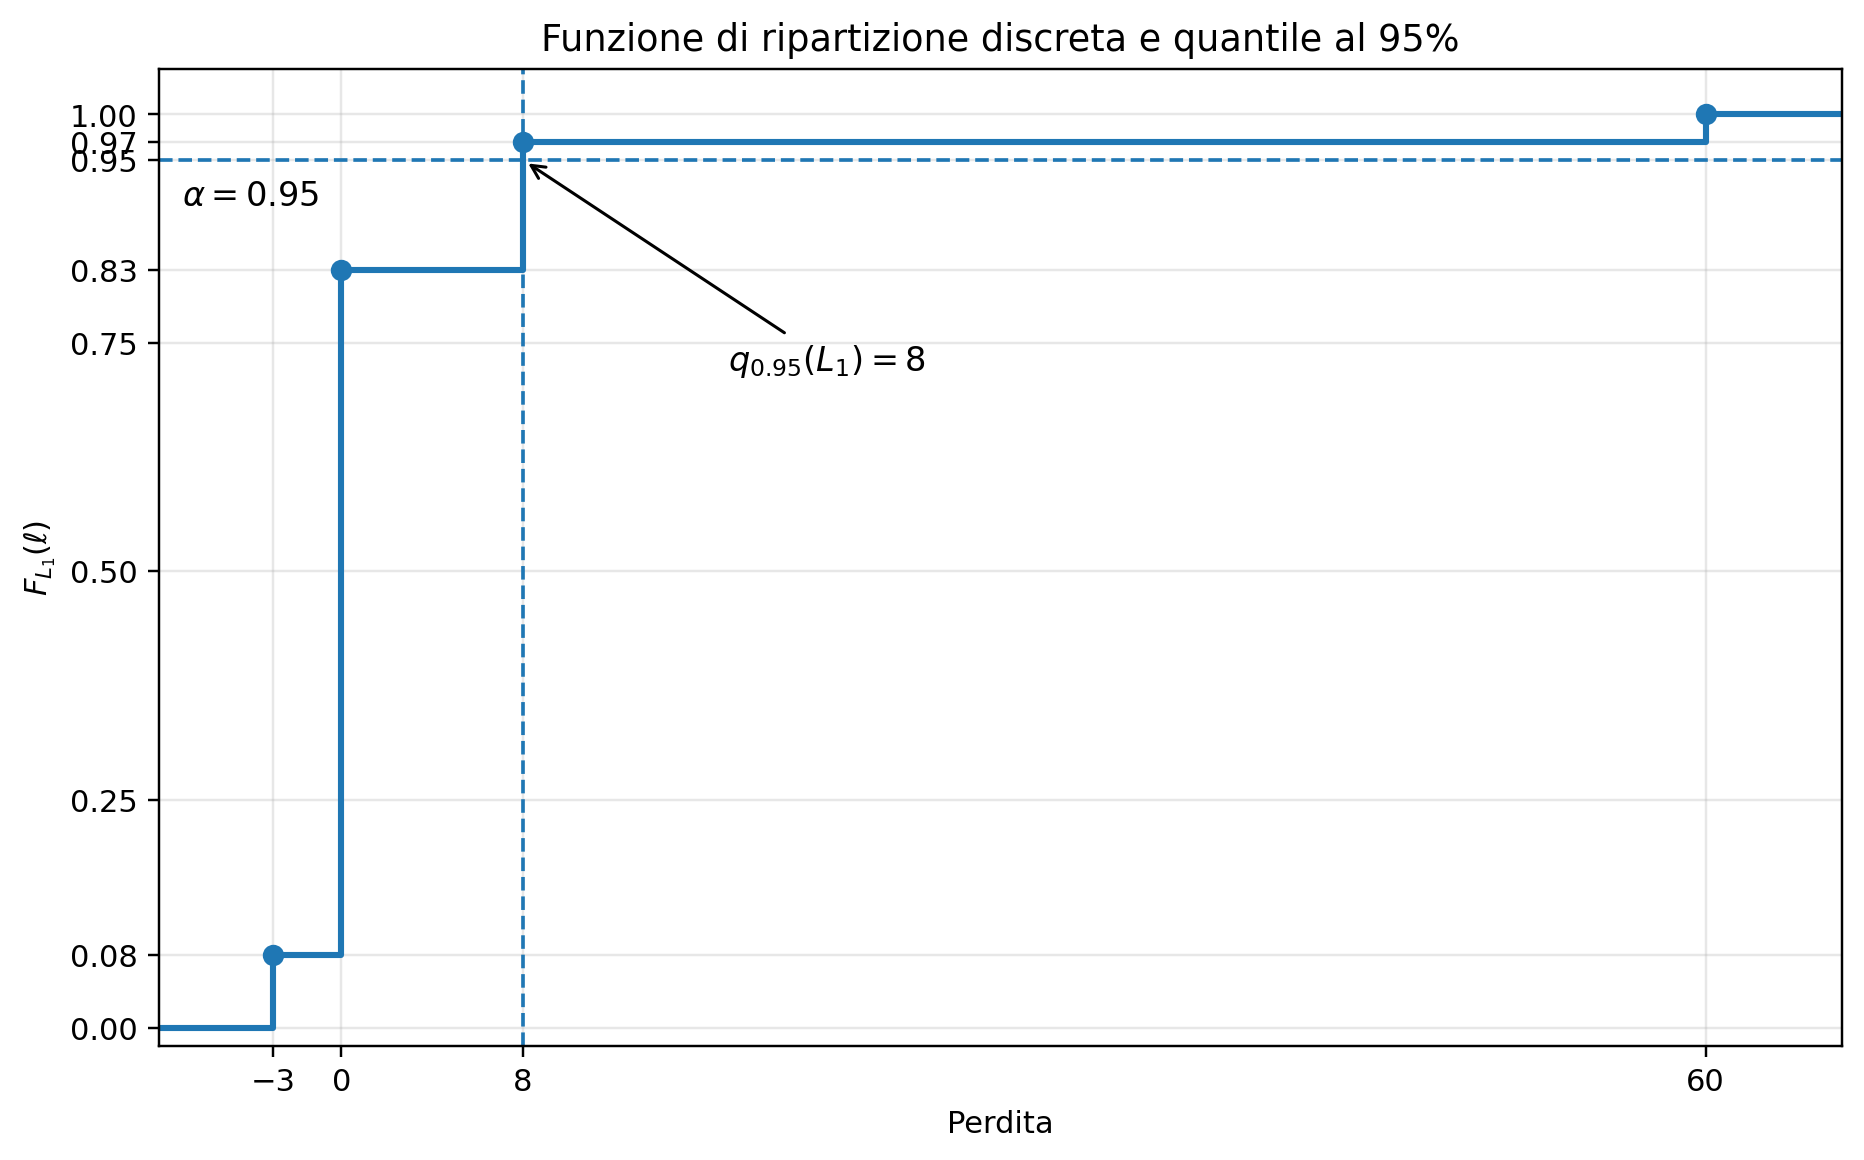
\includegraphics[width=0.82\textwidth]
{../graphics/Cap09_funzione_ripartizione_quantile.png}
\caption{Funzione di ripartizione discreta della perdita e quantile di
livello $0.95$.}
\label{fig:cap09-cdf-quantile}
\end{figure}

La discrezione della distribuzione produce anche variazioni discontinue
del quantile al variare di $\alpha$. Nell'esempio,

\[
q_{\alpha}(L_1\mid X_0=2)
=
\begin{cases}
-3,
&
0<\alpha\leq0.08,
\\[1mm]
0,
&
0.08<\alpha\leq0.83,
\\[1mm]
8,
&
0.83<\alpha\leq0.97,
\\[1mm]
60,
&
0.97<\alpha<1.
\end{cases}
\]

Il quantile \textbf{rimane costante} per interi intervalli di livelli di
probabilit\`{a} e cambia bruscamente quando $\alpha$ supera una
probabilit\`{a} cumulata.

Ad esempio,

\[
q_{0.97}(L_1\mid X_0=2)=8,
\]

mentre, per ogni valore anche di poco superiore a $0.97$,

\[
q_{\alpha}(L_1\mid X_0=2)=60.
\]

Una variazione molto piccola del livello di confidenza pu\`{o} quindi
produrre una variazione molto ampia della soglia monetaria. Questa
instabilit\`{a} non costituisce un errore di calcolo: \`{e} una
conseguenza della distribuzione discreta e della ridotta massa di
probabilit\`{a} collocata tra le perdite intermedie e il default.

\begin{remark}
Per calcolare correttamente un quantile discreto occorre:

\begin{enumerate}

\item ordinare le realizzazioni di $L_h$ in senso crescente;

\item associare a ciascuna realizzazione la relativa probabilit\`{a};

\item costruire le probabilit\`{a} cumulate nell'ordine delle perdite;

\item selezionare la prima perdita per la quale la probabilit\`{a}
cumulata raggiunge o supera $\alpha$.

\end{enumerate}
\end{remark}

L'ordinamento deve riguardare le perdite monetarie, non i codici
numerici attribuiti agli stati della catena. Inoltre, la convenzione

\[
q_{\alpha}(L)
=
\inf
\{
\ell:F_L(\ell)\geq\alpha
\}
\]

deve essere dichiarata esplicitamente. In presenza di distribuzioni
discrete, definizioni o algoritmi differenti possono trattare in modo
diverso i punti nei quali $\alpha$ coincide con una probabilit\`{a}
cumulata.

Il quantile appena definito fornisce la base matematica del Value at
Risk. Nella sezione successiva, la stessa quantit\`{a} verr\`{a}
interpretata come soglia di perdita associata a un livello di
confidenza e a un orizzonte temporale determinati.

\section{Value at Risk creditizio}

\label{sec:cap9-var-creditizio}

Il quantile introdotto nella sezione precedente pu\`{o} essere
interpretato come una soglia monetaria di rischio. Nel contesto
creditizio, tale soglia viene denominata \emph{Value at Risk} della
perdita.

\subsection{Definizione}

\label{subsec:cap9-definizione-var}

\begin{definition}
Sia $L$ una variabile casuale perdita e sia $\alpha\in(0,1)$. Il
\emph{Value at Risk} di livello $\alpha$ \`{e}

\[
\VaR_{\alpha}(L)
=
q_{\alpha}(L)
=
\inf
\left\{
\ell\in\R:
F_L(\ell)\geq\alpha
\right\}.
\]
\end{definition}

Per definizione,

\[
\Prob
\left(
L\leq\VaR_{\alpha}(L)
\right)
\geq
\alpha.
\]

In una distribuzione discreta, la probabilit\`{a} pu\`{o} essere
strettamente maggiore di $\alpha$, poich\'{e} la funzione di
ripartizione pu\`{o} superare il livello richiesto mediante un salto.

Condizionatamente allo stato iniziale $X_0=i$, indicheremo con

\[
\VaR_{\alpha,i}(h)
=
q_{\alpha}(L_h\mid X_0=i)
\]

il VaR della perdita creditizia all'orizzonte $h$.

Nell'esempio della Sezione~9.6,

\[
\VaR_{0.95,2}(1)=8,
\]

poich\'{e}

\[
\Prob(L_1\leq0\mid X_0=2)=0.83<0.95
\]

e

\[
\Prob(L_1\leq8\mid X_0=2)=0.97\geq0.95.
\]

Il risultato indica che $8$ \`{e} la pi\`{u} piccola soglia di perdita
per la quale la probabilit\`{a} cumulata raggiunge almeno il $95\%$.

\subsection{Orizzonte e livello di confidenza}

\label{subsec:cap9-orizzonte-confidenza-var}

Un valore di VaR non \`{e} interpretabile senza specificare almeno:

\begin{itemize}

\item l'orizzonte temporale $h$;

\item il livello di confidenza $\alpha$;

\item la valuta o l'unit\`{a} monetaria della perdita;

\item la distribuzione di $L_h$ e il modello utilizzato per
costruirla.

\end{itemize}

Ad esempio, l'affermazione

\begin{quote}
\emph{il VaR \`{e} pari a 8}
\end{quote}

\noindent
\`{e} incompleta. Una formulazione corretta \`{e}:

\begin{quote}
\emph{Il VaR al $95\%$ della perdita a un anno, condizionatamente al
rating iniziale $i=2$, \`{e} pari a 8 unit\`{a} monetarie nel modello
di transizione del rating considerato.}
\end{quote}

Una variazione dell'orizzonte modifica sia le probabilit\`{a} degli
stati futuri, attraverso $P^h$, sia i valori associati ai rating,
attraverso la funzione $\ell(j,h)$. Pertanto,

\[
\VaR_{\alpha,i}(h)
\]

dipende congiuntamente dal modello delle transizioni e dal modello
delle conseguenze economiche.

\subsection{Credit VaR ed economic capital}

\label{subsec:cap9-credit-var-capitale}

L'espressione \emph{Credit VaR} non viene utilizzata in modo
perfettamente uniforme. Essa pu\`{o} indicare:

\begin{itemize}

\item il quantile della distribuzione della perdita totale;

\item la perdita inattesa quantilica, ottenuta sottraendo la perdita
attesa dal quantile.

\end{itemize}

Nel presente capitolo adotteremo la seguente convenzione:

\[
\mathrm{CreditVaR}_{\alpha,i}(h)
=
\VaR_{\alpha,i}(h),
\]

ossia il Credit VaR coincide con il quantile della perdita totale.

Il capitale economico associato al livello $\alpha$ viene invece
definito come

\[
\mathrm{EC}_{\alpha,i}(h)
=
\VaR_{\alpha,i}(h)
-
\mathrm{EL}_i(h).
\]

La distinzione \`{e} quindi

\[
\begin{array}{lll}
\VaR_{\alpha,i}(h)
&
&
\text{perdita corrispondente al quantile $\alpha$,}
\\[2mm]
\mathrm{EL}_i(h)
&
&
\text{perdita media,}
\\[2mm]
\mathrm{EC}_{\alpha,i}(h)
&
&
\text{perdita quantilica eccedente la media.}
\end{array}
\]

Nell'esempio precedente,

\[
\mathrm{EL}_2(1)=2.68
\]

e

\[
\VaR_{0.95,2}(1)=8.
\]

Pertanto,

\[
\mathrm{EC}_{0.95,2}(1)
=
8-2.68
=
5.32.
\]

Il valore $5.32$ rappresenta la distanza tra la soglia di perdita al
$95\%$ e il costo medio probabilistico dell'esposizione.

\subsection{Limiti del VaR}

\label{subsec:cap9-limiti-var}

Il VaR fornisce una soglia monetaria associata a un livello di
confidenza e a un orizzonte temporale. Questa immediatezza ne facilita
l'interpretazione e la comunicazione, ma non deve nascondere alcuni
limiti importanti.

\medskip

\noindent
\textbf{Il VaR non rappresenta la massima perdita possibile.}

Poniamo

\[
v=\VaR_{\alpha}(L).
\]

Per definizione,

\[
\Prob(L\leq v)\geq\alpha.
\]

Di conseguenza,

\[
\Prob(L>v)\leq 1-\alpha.
\]

Quindi almeno una quota
$1-\alpha$ della distribuzione sar\`{a} associata a perdite superiori a
$v$ e la domanda:

\begin{quote}
\emph{Il VaR costituisce un limite superiore della perdita?}
\end{quote}

\noindent deve ricevere risposta negativa. Il VaR indica una soglia della
distribuzione, non la perdita massima realizzabile.

\medskip

\noindent
\textbf{Il VaR non descrive la severit\`{a} delle perdite oltre la
soglia.}

Una volta determinato il quantile $v$, il VaR non utilizza
l'informazione relativa all'ammontare delle perdite superiori a tale
valore. Se la parte estrema della distribuzione diventa pi\`{u} severa,
ma il quantile di livello $\alpha$ rimane invariato, anche il VaR
rimane invariato.

Due distribuzioni possono pertanto avere lo stesso VaR e presentare
perdite molto differenti negli scenari pi\`{u} sfavorevoli. Il VaR
individua il punto nel quale viene raggiunto il livello di probabilit\`{a}
$\alpha$, ma non misura la gravit\`{a} della coda successiva.

\medskip

\noindent
\textbf{Il VaR pu\`{o} non essere subadditivo.}

Una misura di rischio \`{e} subadditiva se, per due perdite $L_A$ e
$L_B$,

\[
\VaR_{\alpha}(L_A+L_B)
\leq
\VaR_{\alpha}(L_A)
+
\VaR_{\alpha}(L_B).
\]

La propriet\`{a} esprime l'idea che il rischio della posizione
aggregata non debba superare la somma dei rischi misurati separatamente.

Consideriamo ora un esempio autonomo, distinto da quelli sviluppati
nelle sezioni precedenti. Siano $L_A$ e $L_B$ le perdite relative a
due esposizioni indipendenti, entrambe caratterizzate dalla
distribuzione

\[
\begin{array}{c|cc}
\text{perdita}
&
0
&
10
\\
\hline
\text{probabilit\`{a}}
&
0.96
&
0.04
\end{array}
\]

Al livello $\alpha=0.95$,

\[
\VaR_{0.95}(L_A)
=
\VaR_{0.95}(L_B)
=
0,
\]

poich\'{e} per ciascuna esposizione

\[
\Prob(L_A\leq0)
=
\Prob(L_B\leq0)
=
0.96
\geq
0.95.
\]

La perdita aggregata $L_A+L_B$ pu\`{o} assumere i valori $0$, $10$ e
$20$. Per l'indipendenza, la sua distribuzione \`{e}

\[
\begin{array}{c|ccc}
\text{perdita aggregata}
&
0
&
10
&
20
\\
\hline
\text{probabilit\`{a}}
&
(0.96)^2
&
2(0.96)(0.04)
&
(0.04)^2
\\
\hline
&
0.9216
&
0.0768
&
0.0016
\end{array}
\]

La probabilit\`{a} cumulata in corrispondenza della perdita nulla
\`{e}

\[
\Prob(L_A+L_B\leq0)
=
0.9216
<
0.95.
\]

In corrispondenza della perdita $10$ si ha invece

\[
\begin{split}
\Prob(L_A+L_B\leq10)
&=
0.9216+0.0768
\\
&=
0.9984
\geq
0.95.
\end{split}
\]

Pertanto,

\[
\VaR_{0.95}(L_A+L_B)=10.
\]

Ne segue

\[
\VaR_{0.95}(L_A+L_B)
=
10
>
0
=
\VaR_{0.95}(L_A)
+
\VaR_{0.95}(L_B).
\]

In questo esempio il VaR viola la subadditivit\`{a}: la misura
attribuita alla posizione aggregata supera la somma delle misure
attribuite alle due esposizioni considerate separatamente.

\medskip

\noindent
\textbf{Il VaR pu\`{o} essere instabile nelle distribuzioni discrete.}

Torniamo ora alla distribuzione della perdita utilizzata nelle sezioni
precedenti. Le probabilit\`{a} cumulate associate alle perdite $8$ e
$60$ sono rispettivamente

\[
F_{L_1\mid 2}(8)=0.97
\]

e

\[
F_{L_1\mid 2}(60)=1.
\]

Di conseguenza,

\[
\VaR_{0.97,2}(1)=8,
\]

mentre, per ogni $\alpha>0.97$,

\[
\VaR_{\alpha,2}(1)=60.
\]

Un incremento anche molto piccolo del livello di confidenza pu\`{o}
quindi produrre un ampio salto della soglia monetaria. Questo
comportamento deriva dai salti della funzione di ripartizione e dalla
massa di probabilit\`{a} associata al default.

I limiti esaminati mostrano che il VaR non contiene tutta
l'informazione necessaria per valutare il rischio della coda. In
particolare, non misura l'ammontare medio delle perdite pi\`{u}
sfavorevoli. Questa informazione sar\`{a} fornita dalil CVaR, o
Expected Shortfall.

\section{CVaR ed Expected Shortfall}

\label{sec:cap9-cvar-expected-shortfall}

Il VaR individua una soglia della distribuzione, ma non descrive la
gravit\`{a} delle perdite che la superano. Per misurare anche la
severit\`{a} della coda si introduce il CVaR, normalmente denominato
anche \emph{Expected Shortfall}.

\subsection{Definizione mediante quantili}

\label{subsec:cap9-definizione-cvar}

\begin{definition}
Sia $L$ una variabile casuale perdita e sia $\alpha\in(0,1)$. Il
\emph{Conditional Value at Risk} di livello $\alpha$ \`{e}

\[
\CVaR_{\alpha}(L)
=
\frac{1}{1-\alpha}
\int_{\alpha}^{1}
q_u(L)\,du.
\]
\end{definition}

Il CVaR rappresenta la media dei quantili appartenenti alla frazione
$1-\alpha$ pi\`{u} sfavorevole della distribuzione.

Nel presente corso adotteremo la convenzione

\[
\operatorname{ES}_{\alpha}(L)
=
\CVaR_{\alpha}(L),
\]

utilizzando quindi \emph{Expected Shortfall} e CVaR come denominazioni
della stessa misura di rischio.

Per una perdita all'orizzonte $h$, condizionatamente allo stato
iniziale $X_0=i$, scriveremo

\[
\CVaR_{\alpha,i}(h)
=
\CVaR_{\alpha}(L_h\mid X_0=i).
\]

A differenza del VaR, Il CVaR dipende non soltanto dal punto in cui
inizia la coda, ma anche dall'ampiezza delle perdite che la
costituiscono.

\subsection{Rappresentazione di ottimizzazione}

\label{subsec:cap9-rappresentazione-ottimizzazione-cvar}

Il CVaR ammette la rappresentazione

\[
\boxed{
\CVaR_{\alpha}(L)
=
\min_{\eta\in\R}
\left\{
\eta
+
\frac{1}{1-\alpha}
\E\left[(L-\eta)^+\right]
\right\},
}
\]

dove

\[
(x)^+
=
\max\{x,0\}.
\]

Per un valore assegnato di $\eta$, il termine

\[
(L-\eta)^+
\]

misura soltanto l'eccesso della perdita rispetto alla soglia $\eta$.
Le realizzazioni inferiori alla soglia non producono alcun contributo.

La funzione

\[
\eta
\longmapsto
\eta
+
\frac{1}{1-\alpha}
\E\left[(L-\eta)^+\right]
\]

\`{e} convessa. Un suo minimizzatore pu\`{o} essere scelto tra i
quantili di livello $\alpha$; nelle distribuzioni discrete il
minimizzatore pu\`{o} non essere unico.

Questa rappresentazione sar\`{a} particolarmente utile quando il CVaR
verr\`{a} inserita nella funzione obiettivo o nei vincoli di un
problema di ottimizzazione.

\subsection{Distribuzioni discrete e massa nel punto di VaR}

\label{subsec:cap9-cvar-discreta}

Nelle distribuzioni continue, sotto opportune condizioni, il CVaR
pu\`{o} essere interpretata come perdita media condizionata al
superamento del VaR. Questa interpretazione non \`{e} generalmente
corretta nelle distribuzioni discrete.

Poniamo

\[
v
=
\VaR_{\alpha}(L).
\]

Se la funzione di ripartizione presenta un salto nel punto $v$, il
livello $\alpha$ pu\`{o} trovarsi all'interno della massa di
probabilit\`{a} associata a $L=v$. In tal caso,

\[
\CVaR_{\alpha}(L)
=
\frac{
v\left[F_L(v)-\alpha\right]
+
\E\left[
L\1_{\{L>v\}}
\right]
}{
1-\alpha
}.
\]

La formula comprende:

\begin{itemize}

\item tutte le perdite strettamente superiori al VaR;

\item soltanto la frazione della massa nel punto di VaR necessaria a
completare la probabilit\`{a} di coda $1-\alpha$.

\end{itemize}

Riprendiamo la distribuzione utilizzata nelle sezioni precedenti:

\[
\begin{array}{c|cccc}
L_1
&
-3
&
0
&
8
&
60
\\
\hline
\Prob(L_1=\ell\mid X_0=2)
&
0.08
&
0.75
&
0.14
&
0.03
\\
\hline
F_{L_1\mid 2}(\ell)
&
0.08
&
0.83
&
0.97
&
1.00
\end{array}
\]

Al livello $\alpha=0.95$, dalla riga della funzione di ripartizione si
osserva che

\[
F_{L_1\mid 2}(0)=0.83<0.95,
\qquad
F_{L_1\mid 2}(8)=0.97\geq0.95.
\]

Pertanto,

\[
\VaR_{0.95,2}(1)=8.
\]

Il CVaR considera la coda pi\`{u} sfavorevole della distribuzione,
avente probabilit\`{a}

\[
1-\alpha=0.05.
\]

La funzione di ripartizione raggiunge il valore $0.97$ in
corrispondenza della perdita $8$. La parte della coda compresa tra i
livelli $0.95$ e $0.97$ ha quindi probabilit\`{a}

\[
F_{L_1\mid 2}(8)-\alpha
=
0.97-0.95
=
0.02
\]

ed \`{e} associata alla perdita $8$.

La parte restante della coda, compresa tra i livelli $0.97$ e $1$, ha
probabilit\`{a}

\[
1-F_{L_1\mid 2}(8)
=
1-0.97
=
0.03
\]

ed \`{e} associata alla perdita $60$.

Normalizzando queste probabilit\`{a} rispetto alla massa complessiva
della coda, si ottengono le probabilit\`{a} condizionate

\[
\frac{0.02}{0.05}=0.40,
\qquad
\frac{0.03}{0.05}=0.60.
\]

Il CVaR \`{e} quindi il valore atteso condizionato alla coda
pi\`{u} sfavorevole di probabilit\`{a} $0.05$:

\[
\begin{split}
\CVaR_{0.95,2}(1)
&=
8\left(\frac{0.02}{0.05}\right)
+
60\left(\frac{0.03}{0.05}\right)
\\
&=
39.2.
\end{split}
\]

La probabilit\`{a} $0.02$ rappresenta la parte della massa collocata
nel punto di VaR che deve essere inclusa per completare la coda di
probabilit\`{a} $0.05$. Non viene quindi utilizzata l'intera
probabilit\`{a} $0.14$ associata alla perdita $8$.

Per questo motivo, nelle distribuzioni discrete il CVaR non coincide
in generale con

\[
\E
\left[
L_1
\mid
L_1\geq\VaR_{0.95}(L_1)
\right],
\]

poich\'{e} tale condizionamento includerebbe tutta la massa collocata
nel punto di VaR, anzich\'{e} soltanto la frazione necessaria a
costruire la coda di probabilit\`{a} $1-\alpha$.

Lo stesso risultato si ottiene dalla rappresentazione di
ottimizzazione, ponendo $\eta=8$:

\[
\begin{split}
\CVaR_{0.95,2}(1)
&=
8
+
\frac{1}{0.05}
\E\left[(L_1-8)^+\mid X_0=2\right]
\\
&=
8
+
\frac{1}{0.05}(60-8)(0.03)
\\
&=
39.2.
\end{split}
\]

Non sarebbe invece corretto calcolare semplicemente

\[
\E[L_1\mid L_1\geq8,\ X_0=2].
\]

Infatti,

\[
\begin{split}
\E[L_1\mid L_1\geq8,\ X_0=2]
&=
\frac{
(8)(0.14)+(60)(0.03)
}{
0.14+0.03
}
\\
&\approx
17.18,
\end{split}
\]

che non coincide con il CVaR. Il condizionamento $L_1\geq8$ include
l'intera massa di probabilit\`{a} associata alla perdita $8$, mentre
la coda al $5\%$ ne richiede soltanto una parte.

In generale, quindi,

\[
\boxed{
\CVaR_{\alpha}(L)
\neq
\E
\left[
L\mid L\geq\VaR_{\alpha}(L)
\right]
}
\]

quando la distribuzione presenta una massa nel punto di VaR.

\subsection{Confronto tra VaR e CVaR}

\label{subsec:cap9-confronto-var-cvar}

Consideriamo due distribuzioni di perdita:

\[
\begin{array}{c|cccc}
&
0
&
10
&
20
&
100
\\
\hline
\Prob(L_A=x)
&
0.95
&
0
&
0.05
&
0
\\
\Prob(L_B=x)
&
0.95
&
0.04
&
0
&
0.01
\end{array}
\]

Per entrambe le distribuzioni,

\[
\Prob(L_A\leq0)
=
\Prob(L_B\leq0)
=
0.95.
\]

Pertanto,

\[
\VaR_{0.95}(L_A)
=
\VaR_{0.95}(L_B)
=
0.
\]

Il VaR non distingue quindi le due esposizioni. Le rispettive code
sono per\`{o} differenti.

Per $L_A$, l'intera coda al $5\%$ \`{e} costituita dalla perdita $20$:

\[
\CVaR_{0.95}(L_A)
=
20.
\]

Per $L_B$, la coda comprende una perdita pari a $10$ con probabilit\`{a}
$0.04$ e una perdita pari a $100$ con probabilit\`{a} $0.01$:

\[
\begin{split}
\CVaR_{0.95}(L_B)
&=
\frac{
(10)(0.04)+(100)(0.01)
}{
0.05
}
\\
&=
28.
\end{split}
\]

Si ottiene quindi

\[
\VaR_{0.95}(L_A)
=
\VaR_{0.95}(L_B),
\]

ma

\[
\CVaR_{0.95}(L_A)
<
\CVaR_{0.95}(L_B).
\]

Le due distribuzioni iniziano la propria coda nello stesso punto, ma
$L_B$ presenta perdite estreme pi\`{u} severe. Il VaR individua
soltanto la soglia; il CVaR utilizza anche l'informazione contenuta
oltre tale soglia.

\section{Applicazione integrata: rischio di una singola esposizione}

\label{sec:cap9-applicazione-singola-esposizione}

Le sezioni precedenti hanno introdotto separatamente le probabilit\`{a}
di transizione, la funzione di perdita e le misure di rischio. In
questa sezione gli stessi elementi vengono riuniti in un'unica
applicazione finanziaria.

Riprendiamo la matrice di transizione annuale dei rating introdotta nel
Capitolo~8:

\[
P_R
=
\begin{pmatrix}
0.80 & 0.18 & 0.02 & 0.00\\
0.08 & 0.75 & 0.14 & 0.03\\
0.02 & 0.18 & 0.65 & 0.15\\
0.00 & 0.00 & 0.00 & 1.00
\end{pmatrix},
\]

con stati

\[
\mathcal{I}
=
\{
1=\text{alta qualit\`{a}},
\,
2=\text{qualit\`{a} intermedia},
\,
3=\text{speculative grade},
\,
D=\text{default}
\}.
\]

Lo stato $D$, equivalente allo stato $4$ del Capitolo~8, \`{e}
assorbente. Consideriamo un'obbligazione emessa da un soggetto
inizialmente appartenente alla classe di qualit\`{a} intermedia e
valutiamo il rischio a un anno.

\subsection{Probabilit\`{a} degli stati futuri}

\label{subsec:cap9-applicazione-probabilita-stati}

Lo stato iniziale \`{e}

\[
X_0=2.
\]

Poich\'{e} l'orizzonte \`{e} $h=1$, la distribuzione dei rating futuri
si legge direttamente nella seconda riga di $P_R$:

\[
\Prob(X_1=j\mid X_0=2)
=
\begin{cases}
0.08, & j=1,\\[1mm]
0.75, & j=2,\\[1mm]
0.14, & j=3,\\[1mm]
0.03, & j=D.
\end{cases}
\]

La probabilit\`{a} di default entro un anno coincide con la
probabilit\`{a} marginale di default nel primo periodo:

\[
\mathrm{PD}_{2}^{\mathrm{cum}}(1)
=
\mathrm{PD}_{2}^{\mathrm{marg}}(1)
=
(P_R)_{2D}
=
0.03.
\]

La sola probabilit\`{a} di default non descrive tuttavia l'intera
distribuzione economica dell'esposizione. Con probabilit\`{a} $0.14$
l'emittente subisce un downgrade senza entrare in default, mentre con
probabilit\`{a} $0.08$ ottiene un miglioramento del rating.

\subsection{Valori e perdite per stato}

\label{subsec:cap9-applicazione-valori-perdite}

Consideriamo un'obbligazione con

\[
N=100,
\qquad
C=4,
\qquad
T=5,
\]

dove $N$ \`{e} il valore nominale, $C$ la cedola annuale e $T$ la
scadenza. La valutazione viene effettuata alla data $h=1$,
immediatamente dopo il pagamento della prima cedola; rimangono quindi
quattro pagamenti cedolari e il rimborso finale del capitale.

Assumiamo una struttura piatta dei tassi privi di rischio con

\[
r=0.02
\]

e tassi spread creditizi dipendenti dal rating futuro:

\[
s_1=0.012,
\qquad
s_2=0.020,
\qquad
s_3=0.043.
\]

Il tasso di sconto utilizzato per valutare l'obbligazione nello stato
non-default $j$ \`{e}

\[
y_j=r+s_j.
\]

Il valore condizionato al rating futuro \`{e} quindi

\[
V_j(1)
=
\sum_{k=1}^{4}
\frac{C}{(1+y_j)^k}
+
\frac{N}{(1+y_j)^4},
\qquad
j=1,2,3.
\]

Si ottiene

\[
V_1(1)\approx102.96,
\qquad
V_2(1)=100,
\qquad
V_3(1)\approx92.08.
\]

L'aumento dello spread associato al downgrade riduce il valore
dell'obbligazione anche in assenza di default.

Per lo stato di default assumiamo un recovery rate pari al $40\%$
dell'esposizione:

\[
R=0.40,
\qquad
\mathrm{EAD}_1=100.
\]

Assumendo che il recupero sia disponibile alla data di valutazione, il
valore nello stato di default \`{e}

\[
V_D(1)
=
R \cdot \mathrm{EAD}_1
=
40.
\]

Assumiamo come valore di riferimento il valore corrispondente alla
permanenza nella classe iniziale:

\[
V^{\mathrm{ref}}(1)
=
V_2(1)
=
100.
\]

La funzione di perdita \`{e}

\[
\ell(j,1)
=
V^{\mathrm{ref}}(1)-V_j(1).
\]

I risultati sono riassunti nella tabella seguente:

\[
\begin{array}{cccccc}
\hline
\text{stato}
&
(P_R)_{2j}
&
s_j
&
y_j
&
V_j(1)
&
\ell(j,1)
\\
\hline
1
&
0.08
&
1.20\%
&
3.20\%
&
102.96
&
-2.96
\\
2
&
0.75
&
2.00\%
&
4.00\%
&
100.00
&
0.00
\\
3
&
0.14
&
4.30\%
&
6.30\%
&
92.08
&
7.92
\\
D
&
0.03
&
--
&
--
&
40.00
&
60.00
\\
\hline
\end{array}
\]

Per mantenere leggibili i calcoli e raccordare l'applicazione agli
esempi delle sezioni precedenti, utilizziamo i valori arrotondati

\[
\ell(1,1)=-3,
\qquad
\ell(2,1)=0,
\qquad
\ell(3,1)=8,
\qquad
\ell(D,1)=60.
\]

Le misure che seguono sono calcolate sui valori arrotondati. L'impiego
dei valori non arrotondati produrrebbe differenze numeriche minime,
senza modificare l'ordinamento delle perdite o la loro interpretazione
economica.

\subsection{Distribuzione completa della perdita}

\label{subsec:cap9-applicazione-distribuzione-perdita}

La perdita a un anno \`{e}

\[
L_1
=
\ell(X_1,1).
\]

Condizionatamente al rating iniziale $X_0=2$, la funzione di massa e la
funzione di ripartizione sono:

\[
\begin{array}{c|cccc}
L_1
&
-3
&
0
&
8
&
60
\\
\hline
\Prob(L_1=\ell\mid X_0=2)
&
0.08
&
0.75
&
0.14
&
0.03
\\
\hline
F_{L_1\mid 2}(\ell)
&
0.08
&
0.83
&
0.97
&
1.00
\end{array}
\]

La distribuzione contiene quattro conseguenze economiche distinte:

\[
\begin{array}{lll}
L_1=-3
&
&
\text{guadagno da miglioramento del rating,}
\\[1mm]
L_1=0
&
&
\text{assenza di variazione rispetto al riferimento,}
\\[1mm]
L_1=8
&
&
\text{perdita mark-to-market da downgrade,}
\\[1mm]
L_1=60
&
&
\text{perdita da default al netto del recupero.}
\end{array}
\]

La probabilit\`{a} cumulata raggiunge $0.83$ in corrispondenza della
perdita nulla e $0.97$ in corrispondenza della perdita $8$. Il default
occupa la parte estrema della coda, con probabilit\`{a} $0.03$.

\subsection{Misure di rischio}

\label{subsec:cap9-applicazione-misure-rischio}

La perdita attesa \`{e}

\[
\begin{split}
\mathrm{EL}_2(1)
&=
\E[L_1\mid X_0=2]
\\
&=
(-3)(0.08)
+
(0)(0.75)
+
(8)(0.14)
+
(60)(0.03)
\\
&=
2.68.
\end{split}
\]

Il secondo momento \`{e}

\[
\begin{split}
\E[L_1^2\mid X_0=2]
&=
(-3)^2(0.08)
+
8^2(0.14)
+
60^2(0.03)
\\
&=
117.68.
\end{split}
\]

Pertanto,

\[
\begin{split}
\Var(L_1\mid X_0=2)
&=
117.68-(2.68)^2
\\
&=
110.4976,
\end{split}
\]

e la deviazione standard \`{e}

\[
\sigma_{L,2}(1)
=
\sqrt{110.4976}
\approx
10.51.
\]

Consideriamo ora il livello di confidenza

\[
\alpha=0.95.
\]

Poich\'{e}

\[
F_{L_1\mid 2}(0)=0.83<0.95
\]

e

\[
F_{L_1\mid 2}(8)=0.97\geq0.95,
\]

si ottiene

\[
\VaR_{0.95,2}(1)=8.
\]

Per il calcolo del CVaR, la coda pi\`{u} sfavorevole deve avere
probabilit\`{a} $0.05$. La perdita $60$ occupa una massa pari a
$0.03$; la parte compresa tra i livelli cumulati $0.95$ e $0.97$,
pari a $0.02$, \`{e} associata alla perdita $8$. Normalizzando rispetto
alla probabilit\`{a} complessiva della coda,

\[
\begin{split}
\CVaR_{0.95,2}(1)
&=
8\left(\frac{0.02}{0.05}\right)
+
60\left(\frac{0.03}{0.05}\right)
\\
&=
39.2.
\end{split}
\]

Infine, il capitale economico quantilico \`{e}

\[
\begin{split}
\mathrm{EC}_{0.95,2}(1)
&=
\VaR_{0.95,2}(1)
-
\mathrm{EL}_2(1)
\\
&=
8-2.68
\\
&=
5.32.
\end{split}
\]

Le misure ottenute possono essere raccolte nel prospetto seguente:

\[
\begin{array}{lc}
\hline
\text{misura}
&
\text{valore}
\\
\hline
\mathrm{EL}_2(1)
&
2.68
\\
\Var(L_1\mid X_0=2)
&
110.4976
\\
\sigma_{L,2}(1)
&
10.51
\\
\VaR_{0.95,2}(1)
&
8
\\
\CVaR_{0.95,2}(1)
&
39.2
\\
\mathrm{EC}_{0.95,2}(1)
&
5.32
\\
\hline
\end{array}
\]

\subsection{Interpretazione}

\label{subsec:cap9-applicazione-interpretazione}

La perdita attesa pu\`{o} essere scomposta nei contributi associati ai
differenti stati futuri. In termini simbolici,

\[
\begin{split}
\mathrm{EL}_2(1)
&=
\sum_{j\in\mathcal{I}}
\ell(j,1)(P_R)_{2j}
\\
&=
\ell(1,1)(P_R)_{21}
+
\ell(2,1)(P_R)_{22}
\\
&\quad
+
\ell(3,1)(P_R)_{23}
+
\ell(D,1)(P_R)_{2D}.
\end{split}
\]

Sostituendo le perdite e le probabilit\`{a} di transizione,

\[
\begin{split}
\mathrm{EL}_2(1)
&=
\underbrace{(-3)(0.08)}_{\text{upgrade}}
+
\underbrace{(0)(0.75)}_{\text{permanenza}}
\\
&\quad
+
\underbrace{(8)(0.14)}_{\text{downgrade}}
+
\underbrace{(60)(0.03)}_{\text{default}} =2.68.
\end{split}
\]

I quattro contributi sono quindi

\[
-0.24,
\qquad
0,
\qquad
1.12,
\qquad
1.80.
\]

Il default fornisce il contributo positivo maggiore alla perdita
attesa, ma non \`{e} l'unica fonte di rischio. Il downgrade genera una
perdita attesa mark-to-market pari a $1.12$, mentre il miglioramento
del rating produce un guadagno atteso pari a $0.24$ e riduce la perdita
media complessiva.

Il VaR al $95\%$ \`{e} pari a $8$. Tale perdita coincide quindi con la perdita prodotta dal downgrade, non con la perdita da default.
Questo accade perch\'{e} la probabilit\`{a} cumulata raggiunge gi\`{a}
il valore $0.97$ in corrispondenza di $L_1=8$.

La perdita da default, pari a $60$, rimane interamente oltre la soglia
del VaR. Il VaR segnala dove inizia la parte pi\`{u} sfavorevole della
distribuzione, ma non riflette direttamente la distanza tra la perdita
$8$ e la perdita estrema $60$.

Il CVaR, pari a $39.2$, incorpora invece la severit\`{a} della coda. La
coda peggiore del $5\%$ comprende tutti i casi di default, che
rappresentano il $3\%$ della distribuzione, e la frazione necessaria
della massa associata al downgrade. Il valore elevato del CVaR rispetto
al VaR mostra l'importanza della perdita da default negli scenari
estremi.

Infine,

\[
\mathrm{EC}_{0.95,2}(1)=5.32
\]

misura la distanza tra la perdita corrispondente al quantile prefissato e la perdita attesa secondo
la convenzione adottata nel capitolo.

L'applicazione mette cos\`{\i} in evidenza l'intera catena logica:

\[
\boxed{
\begin{array}{c}
\text{matrice di transizione dei rating}
\\
\downarrow
\\
\text{valori condizionati agli stati}
\\
\downarrow
\\
\text{distribuzione della perdita}
\\
\downarrow
\\
\text{EL, VaR, CVaR ed economic capital}.
\end{array}
}
\]

La matrice di transizione costituisce lo scheletro probabilistico del
modello; la valutazione dell'obbligazione e il recovery rate ne
determinano le conseguenze monetarie.

\section{Misura fisica e misura risk-neutral}

\label{sec:cap9-misure-probabilita}

La matrice di transizione attribuisce probabilit\`{a} ai possibili
rating futuri. La scelta delle probabilit\`{a} dipende tuttavia dalla
domanda alla quale il modello deve rispondere.

Occorre distinguere tra:

\[
\text{misurazione del rischio}
\]

e

\[
\text{valutazione di mercato}.
\]

Le due analisi utilizzano lo stesso insieme degli stati creditizi e
possono adottare la stessa struttura markoviana, ma richiedono in
generale matrici di transizione differenti.

Supponiamo, per semplicit\`{a}, che sotto entrambe le misure il rating
segua una catena di Markov omogenea. Indicheremo con

\[
P^{\Prob}
\]

la matrice di transizione sotto la misura fisica e con

\[
P^{\Q}
\]

la matrice di transizione sotto la misura risk-neutral.

\subsection{Due domande differenti}

\label{subsec:cap9-due-domande}

La \emph{misurazione del rischio} considera le probabilit\`{a} con cui
gli stati creditizi possono effettivamente realizzarsi. La domanda
principale \`{e}:

\[
\text{quali perdite possono verificarsi e con quali probabilit\`{a}?}
\]

Questa analisi richiede probabilit\`{a} predittive, riferite
all'evoluzione reale del rating dell'emittente. Le misure di perdita
attesa, VaR e CVaR devono pertanto essere calcolate sotto la misura
fisica $\Prob$.

La \emph{valutazione di mercato} risponde invece alla domanda:

\[
\text{qual \`{e} oggi il valore di mercato dei flussi futuri?}
\]

In un modello di pricing coerente con l'assenza di arbitraggio, il
valore viene ottenuto come valore atteso, sotto la misura
risk-neutral $\Q$, dei flussi futuri opportunamente attualizzati.

La distinzione pu\`{o} essere sintetizzata come segue:

\[
\begin{array}{ccl}
\text{misurazione del rischio}
&
\longrightarrow
&
\text{probabilit\`{a} predittive sotto }\Prob,
\\[2mm]
\text{valutazione di mercato}
&
\longrightarrow
&
\text{valori attesi di flussi attualizzati sotto }\Q.
\end{array}
\]

Le probabilit\`{a} risk-neutral non rappresentano necessariamente le
frequenze con cui gli eventi creditizi si realizzeranno. Esse sono
pesi probabilistici utilizzati per riprodurre i prezzi di mercato.

\subsection{Matrice sotto la misura fisica}

\label{subsec:cap9-matrice-fisica}

Indichiamo con

\[
P^{\Prob}
=
\left(
p_{ij}^{\Prob}
\right)_{i,j\in\mathcal{I}}
\]

la matrice di transizione sotto la misura fisica, dove

\[
p_{ij}^{\Prob}
=
\Prob(X_{t+1}=j\mid X_t=i).
\]

Per una catena omogenea,

\[
\Prob(X_h=j\mid X_0=i)
=
\left[
\left(P^{\Prob}\right)^h
\right]_{ij}.
\]

La matrice $P^{\Prob}$ determina quindi la distribuzione predittiva
degli stati futuri. Data la funzione di perdita $\ell(j,h)$, si
ottiene

\[
\Prob
\left(
L_h=\ell(j,h)
\mid X_0=i
\right)
=
\left[
\left(P^{\Prob}\right)^h
\right]_{ij},
\]

quando stati differenti producono perdite differenti. Se pi\`{u}
stati producono la stessa perdita, le corrispondenti probabilit\`{a}
devono essere aggregate.

La perdita attesa sotto la misura fisica \`{e}

\[
\mathrm{EL}_{i}^{\Prob}(h)
=
\E^{\Prob}[L_h\mid X_0=i]
=
\sum_{j\in\mathcal{I}}
\ell(j,h)
\left[
\left(P^{\Prob}\right)^h
\right]_{ij}.
\]

Anche la funzione di ripartizione della perdita viene costruita
utilizzando le probabilit\`{a} fisiche:

\[
F_{L_h\mid i}^{\Prob}(\lambda)
=
\sum_{\substack{j\in\mathcal{I}:\\
\ell(j,h)\leq\lambda}}
\left[
\left(P^{\Prob}\right)^h
\right]_{ij}.
\]

Da questa distribuzione si ricavano

\[
\VaR_{\alpha,i}^{\Prob}(h)
\]

e

\[
\CVaR_{\alpha,i}^{\Prob}(h).
\]

La sequenza concettuale \`{e} dunque

\[
P^{\Prob}
\longrightarrow
\text{distribuzione predittiva dei rating}
\longrightarrow
\text{distribuzione della perdita}
\longrightarrow
\mathrm{EL}^{\Prob},
\VaR^{\Prob},
\CVaR^{\Prob}.
\]

La matrice fisica pu\`{o} essere stimata, ad esempio, mediante le
frequenze storiche delle transizioni osservate. Il suo impiego
richiede tuttavia cautela, poich\'{e} le frequenze passate possono
non rappresentare correttamente la dinamica futura in presenza di
cambiamenti macroeconomici, istituzionali o nella composizione degli
emittenti.

\subsection{Matrice sotto la misura risk-neutral}

\label{subsec:cap9-matrice-risk-neutral}

Indichiamo con

\[
P^{\Q}
=
\left(
p_{ij}^{\Q}
\right)_{i,j\in\mathcal{I}}
\]

la matrice di transizione sotto la misura risk-neutral, dove

\[
p_{ij}^{\Q}
=
\Q(X_{t+1}=j\mid X_t=i).
\]

Per una catena omogenea sotto $\Q$,

\[
\Q(X_h=j\mid X_0=i)
=
\left[
\left(P^{\Q}\right)^h
\right]_{ij}.
\]

La matrice $P^{\Q}$ non viene utilizzata per prevedere le frequenze
future dei rating. Essa fornisce i pesi probabilistici impiegati nella
valutazione di mercato dei flussi creditizi.

Sia $C_t$ il flusso aleatorio pagato alla data $t$ e sia $D(0,t)$ il
fattore di attualizzazione dalla data $t$ alla data iniziale. Il valore
di mercato al tempo zero \`{e}

\[
V_0
=
\E^{\Q}
\left[
\sum_{t=1}^{T}
D(0,t)C_t
\right].
\]

Nel caso semplificato in cui il fattore di attualizzazione sia
deterministico e il flusso alla data $t$ dipenda soltanto dallo stato
occupato, ossia

\[
C_t=c_t(X_t),
\]

si ottiene

\[
V_0
=
\sum_{t=1}^{T}
D(0,t)
\sum_{j\in\mathcal{I}}
c_t(j)
\left[
\left(P^{\Q}\right)^t
\right]_{ij}.
\]

La struttura rilevante per il pricing \`{e} quindi

\[
P^{\Q}
\longrightarrow
\text{probabilit\`{a} risk-neutral dei flussi}
\longrightarrow
\E^{\Q}
\left[
\text{flussi attualizzati}
\right]
\longrightarrow
\text{valore di mercato}.
\]

In generale,

\[
P^{\Prob}
\neq
P^{\Q}.
\]

Le probabilit\`{a} fisiche riflettono la dinamica predittiva degli
stati creditizi. Le probabilit\`{a} risk-neutral incorporano invece
anche la remunerazione richiesta dal mercato per l'esposizione al
rischio.

Di conseguenza, una matrice stimata mediante frequenze storiche non
pu\`{o} essere utilizzata automaticamente come matrice di pricing. Il
fatto che una matrice descriva adeguatamente le transizioni osservate
non implica che, utilizzata sotto $\Q$, essa riproduca i prezzi delle
obbligazioni creditizie o dei derivati di credito.

\subsection{Portata e limiti della distinzione}

\label{subsec:cap9-portata-misure}

La distinzione tra $\Prob$ e $\Q$ riguarda innanzitutto il ruolo
attribuito alle probabilit\`{a}:

\[
\begin{array}{ccl}
P^{\Prob}
&
:
&
\text{probabilit\`{a} degli scenari futuri},
\\[2mm]
P^{\Q}
&
:
&
\text{pesi probabilistici per la valutazione di mercato}.
\end{array}
\]

Questa separazione non implica tuttavia che la misurazione del rischio
e la valutazione di mercato siano sempre completamente indipendenti.

In un modello di perdita mark-to-market, le probabilit\`{a} con cui si
raggiungono i rating futuri sono generalmente determinate sotto la
misura fisica:

\[
\Prob(X_h=j\mid X_0=i)
=
\left[
\left(P^{\Prob}\right)^h
\right]_{ij}.
\]

Il valore dell'esposizione condizionato allo stato futuro $j$ pu\`{o}
invece essere un valore di mercato, ottenuto alla data $h$ mediante una
valutazione risk-neutral dei flussi successivi. In tal caso,

\[
P^{\Prob}
\longrightarrow
\text{probabilit\`{a} degli scenari},
\]

mentre

\[
P^{\Q}
\longrightarrow
V_j(h).
\]

La perdita all'orizzonte rimane

\[
L_h
=
V^{\mathrm{ref}}(h)-V_{X_h}(h),
\]

ma la sua distribuzione utilizza le probabilit\`{a} fisiche degli
stati, mentre i valori $V_j(h)$ possono incorporare una valutazione di
mercato sotto $\Q$.

Nel seguito assumeremo che la matrice $P^{\Q}$ sia assegnata. La sua
calibrazione a partire dai prezzi di obbligazioni, CDS e altri
strumenti creditizi richiede la specificazione congiunta dei tassi di
interesse, dei flussi contrattuali, del recovery rate e dei premi per
il rischio.

Tali problemi di calibrazione vengono rinviati a corsi specialistici.
Nel presente capitolo la distinzione essenziale \`{e} la seguente:

\[
\boxed{
\begin{array}{c}
P^{\Prob}
\text{ per misurare il rischio,}
\\[2mm]
P^{\Q}
\text{ per valutare i flussi di mercato.}
\end{array}
}
\]

\section{Il credit default swap}

\label{sec:cap9-cds}

La distinzione tra misura fisica e misura risk-neutral diventa
operativa nella valutazione dei derivati di credito. Consideriamo il
\emph{credit default swap}, o CDS, nella sua forma pi\`{u} semplice.

Il CDS \`{e} un contratto nel quale una parte (tipicamente il proprietario di titoli obbligazionari) acquista protezione
contro il verificarsi di un evento creditizio avverso che colpisce l'emittente dei titoli posseduti. In cambio della protezione, essa paga periodicamente un
premio alla controparte.

La valutazione del contratto viene effettuata sotto la misura
risk-neutral $\Q$. Le probabilit\`{a} di default utilizzate nel pricing
sono pertanto ricavate dalla matrice di transizione $P^{\Q}$, non dalla
matrice fisica $P^{\Prob}$.

\subsection{Struttura contrattuale}

\label{subsec:cap9-cds-struttura}

Le parti e gli elementi essenziali di un CDS sono:

\begin{itemize}

\item il \emph{protection buyer}, che acquista la protezione e paga il
premio periodico;

\item il \emph{protection seller}, che riceve i premi e si impegna a
effettuare il pagamento di protezione in caso di evento creditizio;

\item la \emph{reference entity}, ossia l'emittente al cui rischio di
credito \`{e} riferito il contratto;

\item il nozionale $N$, sul quale vengono calcolati sia i premi sia il
pagamento di protezione;

\item il premio periodico, determinato mediante uno spread contrattuale
$s$;

\item il \emph{credit event}, che nel modello semplificato coincide con
il default della reference entity;

\item il \emph{recovery rate} $R$, che determina la parte del nozionale
recuperabile dopo il default;

\item la \emph{scadenza contrattuale} $H$.

\end{itemize}

I flussi del CDS sono suddivisi in due componenti:

\[
\begin{array}{ccl}
\text{gamba dei premi}
&
:
&
\text{pagamenti effettuati dal protection buyer,}
\\[2mm]
\text{gamba di protezione}
&
:
&
\text{pagamento effettuato dal protection seller in caso di default.}
\end{array}
\]

Indichiamo con $\mathrm{PV}_{\mathrm{prot}}$ il valore attuale della
gamba di protezione e con $\mathrm{PV}_{\mathrm{prem}}(s)$ il valore
attuale della gamba dei premi, calcolata per uno spread contrattuale
$s$.

Dal punto di vista del protection buyer, il valore del CDS alla data
iniziale \`{e} quindi

\[
V_{\mathrm{CDS}}(s)
=
\mathrm{PV}_{\mathrm{prot}}
-
\mathrm{PV}_{\mathrm{prem}}(s).
\]

Per il protection seller i segni dei due flussi sono opposti.

Indichiamo con

\[
\tau_D
=
\inf\{h\geq1:X_h=D\}
\]

il tempo di primo ingresso nello stato di default e con $d_h$ il
fattore deterministico di attualizzazione dalla data $h$ alla data
iniziale.

\subsection{Gamba di protezione}

\label{subsec:cap9-cds-protezione}

Se il default si verifica alla data $h$, il protection seller paga al
protection buyer la perdita sul nozionale:

\[
N(1-R).
\]

Il valore attuale del pagamento condizionato all'evento
$\{\tau_D=h\}$ \`{e}

\[
d_hN(1-R).
\]

Poich\'{e} il pagamento viene effettuato soltanto se il primo ingresso
in default avviene alla data $h$, il valore attuale atteso della gamba
di protezione \`{e}

\[
\mathrm{PV}_{\mathrm{prot}}
=
N(1-R)
\sum_{h=1}^{H}
d_h
\Q(\tau_D=h\mid X_0=i).
\]

Le probabilit\`{a} marginali di default sono ottenute dalla matrice
risk-neutral. Poich\'{e} lo stato $D$ \`{e} assorbente,

\[
\Q(\tau_D\leq h\mid X_0=i)
=
\left[
\left(P^{\Q}\right)^h
\right]_{iD},
\]

e quindi

\[
\Q(\tau_D=h\mid X_0=i)
=
\left[
\left(P^{\Q}\right)^h
\right]_{iD}
-
\left[
\left(P^{\Q}\right)^{h-1}
\right]_{iD}.
\]

La gamba di protezione dipende dunque dalle probabilit\`{a} di primo
ingresso in default alle diverse date contrattuali, dal recovery rate
e dai fattori di attualizzazione.

\subsection{Gamba dei premi}

\label{subsec:cap9-cds-premi}

Il protection buyer paga a ogni data $h$ un premio pari a

\[
sN,
\]

purch\'{e} la reference entity sia ancora sopravvissuta oltre tale
data.

Nella convenzione temporale adottata, se il default si verifica
esattamente alla data $h$, il pagamento del premio alla stessa data
non viene effettuato. Il premio alla data $h$ viene quindi pagato
soltanto sull'evento

\[
\{\tau_D>h\}.
\]

Il valore attuale atteso della gamba dei premi \`{e}

\[
\mathrm{PV}_{\mathrm{prem}}(s)
=
sN
\sum_{h=1}^{H}
d_h
\Q(\tau_D>h\mid X_0=i).
\]

Le probabilit\`{a} di sopravvivenza sotto la misura risk-neutral sono

\[
\Q(\tau_D>h\mid X_0=i)
=
1-
\left[
\left(P^{\Q}\right)^h
\right]_{iD}.
\]

Pertanto,

\[
\mathrm{PV}_{\mathrm{prem}}(s)
=
sN
\sum_{h=1}^{H}
d_h
\left\{
1-
\left[
\left(P^{\Q}\right)^h
\right]_{iD}
\right\}.
\]

Il premio contrattuale viene moltiplicato per probabilit\`{a} di
sopravvivenza, poich\'{e} i pagamenti futuri cessano dopo il default
della reference entity.

\subsection{Premio equo del CDS}

\label{subsec:cap9-cds-premio-equilibrio}

Alla data iniziale, il premio equo $s^{*}$ rende nullo il valore del
CDS. Dal punto di vista del protection buyer, deve quindi valere

\[
V_{\mathrm{CDS}}(s^{*})=0,
\]

ossia

\[
\mathrm{PV}_{\mathrm{prem}}(s^{*})
=
\mathrm{PV}_{\mathrm{prot}}.
\]

Sostituendo le espressioni delle due gambe,

\[
s^{*}N
\sum_{h=1}^{H}
d_h
\Q(\tau_D>h\mid X_0=i)
=
N(1-R)
\sum_{h=1}^{H}
d_h
\Q(\tau_D=h\mid X_0=i).
\]

Il nozionale compare in entrambe le gambe e si semplifica. Il premio
equo \`{e} quindi

\[
s^{*}
=
(1-R)
\frac{
\displaystyle
\sum_{h=1}^{H}
d_h
\Q(\tau_D=h\mid X_0=i)
}{
\displaystyle
\sum_{h=1}^{H}
d_h
\Q(\tau_D>h\mid X_0=i)
}.
\]

Il numeratore rappresenta il valore attuale risk-neutral della perdita
unitaria attesa da default:

\[
(1-R)
\sum_{h=1}^{H}
d_h
\Q(\tau_D=h\mid X_0=i).
\]

Il denominatore rappresenta invece il valore attuale atteso di
un'unit\`{a} di premio pagata alle date nelle quali l'emittente
sopravvive:

\[
\sum_{h=1}^{H}
d_h
\Q(\tau_D>h\mid X_0=i).
\]

Il premio equo aumenta, a parit\`{a} delle altre condizioni, quando
aumentano le probabilit\`{a} risk-neutral di default o quando
diminuisce il recovery rate.

La relazione pu\`{o} essere sintetizzata come

\[
\boxed{
\text{premio equo}
=
\frac{
\text{valore attuale atteso della protezione}
}{
\text{valore attuale atteso dell'unit\`{a} di premio}
}.
}
\]

\subsection{Ipotesi semplificatrici}

\label{subsec:cap9-cds-ipotesi}

La formulazione precedente ha finalit\`{a} didattica e si basa sulle
seguenti ipotesi:

\begin{itemize}

\item le date di pagamento e di possibile default sono annuali;

\item i tassi di interesse e i fattori di attualizzazione $d_h$ sono
deterministici;

\item il recovery rate $R$ \`{e} costante;

\item il pagamento della protezione avviene alla data discreta nella
quale viene rilevato il default;

\item non viene corrisposto il premio maturato tra l'ultima data di
pagamento e la data di default;

\item se il default avviene alla data $h$, il premio previsto alla
stessa data non viene pagato;

\item il protection seller \`{e} privo di rischio di controparte;

\item non sono considerati collateral, margini, costi di transazione o
altri aggiustamenti di valutazione.

\end{itemize}

Nei contratti di mercato i premi sono normalmente pagati con frequenza
inferiore all'anno, il default pu\`{o} verificarsi tra due date di
pagamento e il premio maturato deve essere trattato esplicitamente.
Questi elementi modificano il dettaglio dei flussi, ma non la logica
fondamentale del pricing:

\[
\text{valore della gamba dei premi}
=
\text{valore della gamba di protezione}.
\]

La matrice $P^{\Q}$ collega quindi la dinamica risk-neutral dei rating
al valore del CDS:

\[
\boxed{
P^{\Q}
\longrightarrow
\begin{array}{c}
\text{probabilit\`{a} di default}
\\
\text{e di sopravvivenza}
\end{array}
\longrightarrow
\begin{array}{c}
\text{gamba di protezione}
\\
\text{e gamba dei premi}
\end{array}
\longrightarrow
s^{*}.
}
\]

\section{Copertura mediante CDS e rischio residuo}

\label{sec:cap9-copertura-cds}

Un CDS pu\`{o} essere utilizzato per ridurre le perdite associate al
default di un'esposizione creditizia. La copertura non elimina tuttavia
necessariamente tutte le componenti del rischio: il risultato dipende
dal nozionale protetto, dalla scadenza, dalla definizione contrattuale
del credit event e dalla relazione tra il valore dell'esposizione e
quello del CDS.

La distinzione tra misura fisica e misura risk-neutral rimane
essenziale. Il premio del CDS viene determinato mediante probabilit\`{a}
risk-neutral, mentre la distribuzione delle perdite della posizione
coperta deve essere valutata mediante probabilit\`{a} fisiche.

Tutte le componenti monetarie considerate nel seguito sono espresse
alla medesima data di valutazione.

\subsection{Posizione non coperta}

\label{subsec:cap9-posizione-non-coperta}

Indichiamo con $L^{\mathrm{credito}}$ la perdita dell'esposizione
creditizia in assenza di strumenti di copertura.

La perdita della posizione non coperta \`{e} quindi

\[
L^{\mathrm{unhedged}}
=
L^{\mathrm{credito}}.
\]

La sua distribuzione dipende dalle probabilit\`{a} fisiche degli stati
creditizi futuri e dalla funzione che associa a ogni stato il valore
dell'esposizione.

Nel caso dell'applicazione della Sezione~9.9,

\[
L^{\mathrm{unhedged}}
\in
\{-3,0,8,60\},
\]

con distribuzione

\[
\begin{array}{c|cccc}
L^{\mathrm{unhedged}}
&
-3
&
0
&
8
&
60
\\
\hline
\Prob
\left(
L^{\mathrm{unhedged}}=\ell
\mid X_0=2
\right)
&
0.08
&
0.75
&
0.14
&
0.03.
\end{array}
\]

La perdita da default \`{e} pari a $60$, mentre la perdita da downgrade
\`{e} pari a $8$.

\subsection{Posizione coperta}

\label{subsec:cap9-posizione-coperta}

Indichiamo con $\Pi^{\mathrm{CDS}}$ il pagamento ricevuto dal CDS e con
$C^{\mathrm{premi}}$ il costo complessivo dei premi. Dal punto di vista
del protection buyer, la perdita della posizione coperta \`{e}

\[
L^{\mathrm{hedged}}
=
L^{\mathrm{credito}}
-
\Pi^{\mathrm{CDS}}
+
C^{\mathrm{premi}}.
\]

Il pagamento del CDS riduce la perdita, mentre il costo dei premi la
aumenta.

Nella rappresentazione semplificata con copertura del solo default,

\[
\Pi^{\mathrm{CDS}}
=
N_{\mathrm{CDS}}
\left(
1-R_{\mathrm{CDS}}
\right)
\1_{\{\tau_D\leq H\}},
\]

dove $N_{\mathrm{CDS}}$ \`{e} il nozionale del contratto e
$R_{\mathrm{CDS}}$ il recovery rate previsto ai fini del regolamento
della protezione.

La copertura \`{e} completa rispetto alla perdita da default soltanto
se

\[
N_{\mathrm{CDS}}
\left(
1-R_{\mathrm{CDS}}
\right)
\]

coincide con la perdita effettivamente subita sull'esposizione in caso
di default. Anche in questo caso rimangono il costo dei premi e le
eventuali perdite prodotte dalle variazioni del merito creditizio che
non determinano un credit event.

Prendendo il valore atteso sotto la misura fisica, si ottiene

\[
\begin{split}
\E^{\Prob}
\left[
L^{\mathrm{hedged}}
\right]
&=
\E^{\Prob}
\left[
L^{\mathrm{unhedged}}
\right]
-
\E^{\Prob}
\left[
\Pi^{\mathrm{CDS}}
\right]
\\
&\quad
+
\E^{\Prob}
\left[
C^{\mathrm{premi}}
\right].
\end{split}
\]

Pertanto, la variazione della perdita attesa \`{e}

\[
\E^{\Prob}
\left[
L^{\mathrm{hedged}}
\right]
-
\E^{\Prob}
\left[
L^{\mathrm{unhedged}}
\right]
=
\E^{\Prob}
\left[
C^{\mathrm{premi}}
\right]
-
\E^{\Prob}
\left[
\Pi^{\mathrm{CDS}}
\right].
\]

La copertura riduce la perdita attesa soltanto quando il valore atteso
fisico della protezione supera il costo atteso dei premi. Questa
condizione non \`{e} garantita dal fatto che il CDS sia stato stipulato
a un premio equo sotto la misura risk-neutral.

\subsection{Confronto delle distribuzioni}

\label{subsec:cap9-confronto-distribuzioni-copertura}

Il confronto tra posizione coperta e non coperta non pu\`{o} limitarsi
alla perdita attesa. Occorre ricostruire l'intera distribuzione di

\[
L^{\mathrm{hedged}}
=
L^{\mathrm{credito}}
-
\Pi^{\mathrm{CDS}}
+
C^{\mathrm{premi}}
\]

e calcolare separatamente

\[
\E^{\Prob}
\left[
L^{\mathrm{hedged}}
\right],
\qquad
\VaR_{\alpha}^{\Prob}
\left(
L^{\mathrm{hedged}}
\right),
\qquad
\CVaR_{\alpha}^{\Prob}
\left(
L^{\mathrm{hedged}}
\right).
\]

In generale, non valgono relazioni additive semplici per il VaR e il
CVaR. Il pagamento del CDS, la perdita creditizia e il costo dei premi
dipendono infatti dagli stessi eventi creditizi.

Consideriamo un esempio costruito sulla distribuzione della
Sezione~9.9. Supponiamo che il CDS:

\begin{itemize}

\item paghi $60$ in caso di default;

\item non effettui alcun pagamento negli altri stati;

\item richieda un premio unico anticipato, espresso in valore
equivalente alla data di analisi, pari a $2$.

\end{itemize}

Si ha quindi

\[
\Pi^{\mathrm{CDS}}
=
60\1_{\{X_1=D\}},
\qquad
C^{\mathrm{premi}}=2.
\]

La perdita della posizione coperta nei differenti stati \`{e}

\[
\begin{array}{c|ccccc}
\text{stato}
&
\Prob(X_1=j\mid X_0=2)
&
L^{\mathrm{credito}}
&
\Pi^{\mathrm{CDS}}
&
C^{\mathrm{premi}}
&
L^{\mathrm{hedged}}
\\
\hline
1
&
0.08
&
-3
&
0
&
2
&
-1
\\
2
&
0.75
&
0
&
0
&
2
&
2
\\
3
&
0.14
&
8
&
0
&
2
&
10
\\
D
&
0.03
&
60
&
60
&
2
&
2
\end{array}
\]

La protezione elimina la perdita lorda da default, ma il costo del
premio rimane anche nello stato di default. Inoltre, negli stati
non-default, il premio si aggiunge alla perdita o riduce il guadagno
della posizione creditizia.

Poich\'{e} gli stati $2$ e $D$ producono entrambi una perdita coperta
pari a $2$, le loro probabilit\`{a} devono essere aggregate. La
distribuzione della posizione coperta \`{e}

\[
\begin{array}{c|ccc}
L^{\mathrm{hedged}}
&
-1
&
2
&
10
\\
\hline
\Prob
\left(
L^{\mathrm{hedged}}=\ell
\mid X_0=2
\right)
&
0.08
&
0.78
&
0.14
\\
\hline
F_{L^{\mathrm{hedged}}\mid 2}(\ell)
&
0.08
&
0.86
&
1.00.
\end{array}
\]

La perdita attesa della posizione coperta si ottiene sommando ciascun
possibile valore della perdita, ponderato per la corrispondente
probabilit\`{a}. In termini simbolici,

\[
\E^{\Prob}
\left[
L^{\mathrm{hedged}}
\mid X_0=2
\right]
=
\sum_{\lambda\in\mathcal{L}^{\mathrm{hedged}}}
\lambda
\Prob
\left(
L^{\mathrm{hedged}}=\lambda
\mid X_0=2
\right),
\]

dove

\[
\mathcal{L}^{\mathrm{hedged}}
=
\{-1,2,10\}.
\]

Sostituendo i valori della distribuzione,

\[
\begin{split}
\E^{\Prob}
\left[
L^{\mathrm{hedged}}
\mid X_0=2
\right]
&=
(-1)(0.08)
+
(2)(0.78)
+
(10)(0.14)
\\
&=
2.88.
\end{split}
\]

Il medesimo risultato pu\`{o} essere ottenuto osservando che

\[
\E^{\Prob}
\left[
\Pi^{\mathrm{CDS}}
\mid X_0=2
\right]
=
(60)(0.03)
=
1.80.
\]

Pertanto,

\[
\begin{split}
\E^{\Prob}
\left[
L^{\mathrm{hedged}}
\mid X_0=2
\right]
&=
2.68-1.80+2
\\
&=
2.88.
\end{split}
\]

Al livello $\alpha=0.95$,

\[
F_{L^{\mathrm{hedged}}\mid 2}(2)
=
0.86
<
0.95,
\]

mentre

\[
F_{L^{\mathrm{hedged}}\mid 2}(10)
=
1
\geq
0.95.
\]

Di conseguenza,

\[
\VaR_{0.95}^{\Prob}
\left(
L^{\mathrm{hedged}}
\right)
=
10.
\]

La coda peggiore di probabilit\`{a} $0.05$ \`{e} interamente
contenuta nella massa associata alla perdita $10$. Pertanto,

\[
\CVaR_{0.95}^{\Prob}
\left(
L^{\mathrm{hedged}}
\right)
=
10.
\]
come evidenziato nella figura \ref{fig:cap09-cdf-hedged-var-cvar}

\begin{figure}[htbp]
\centering
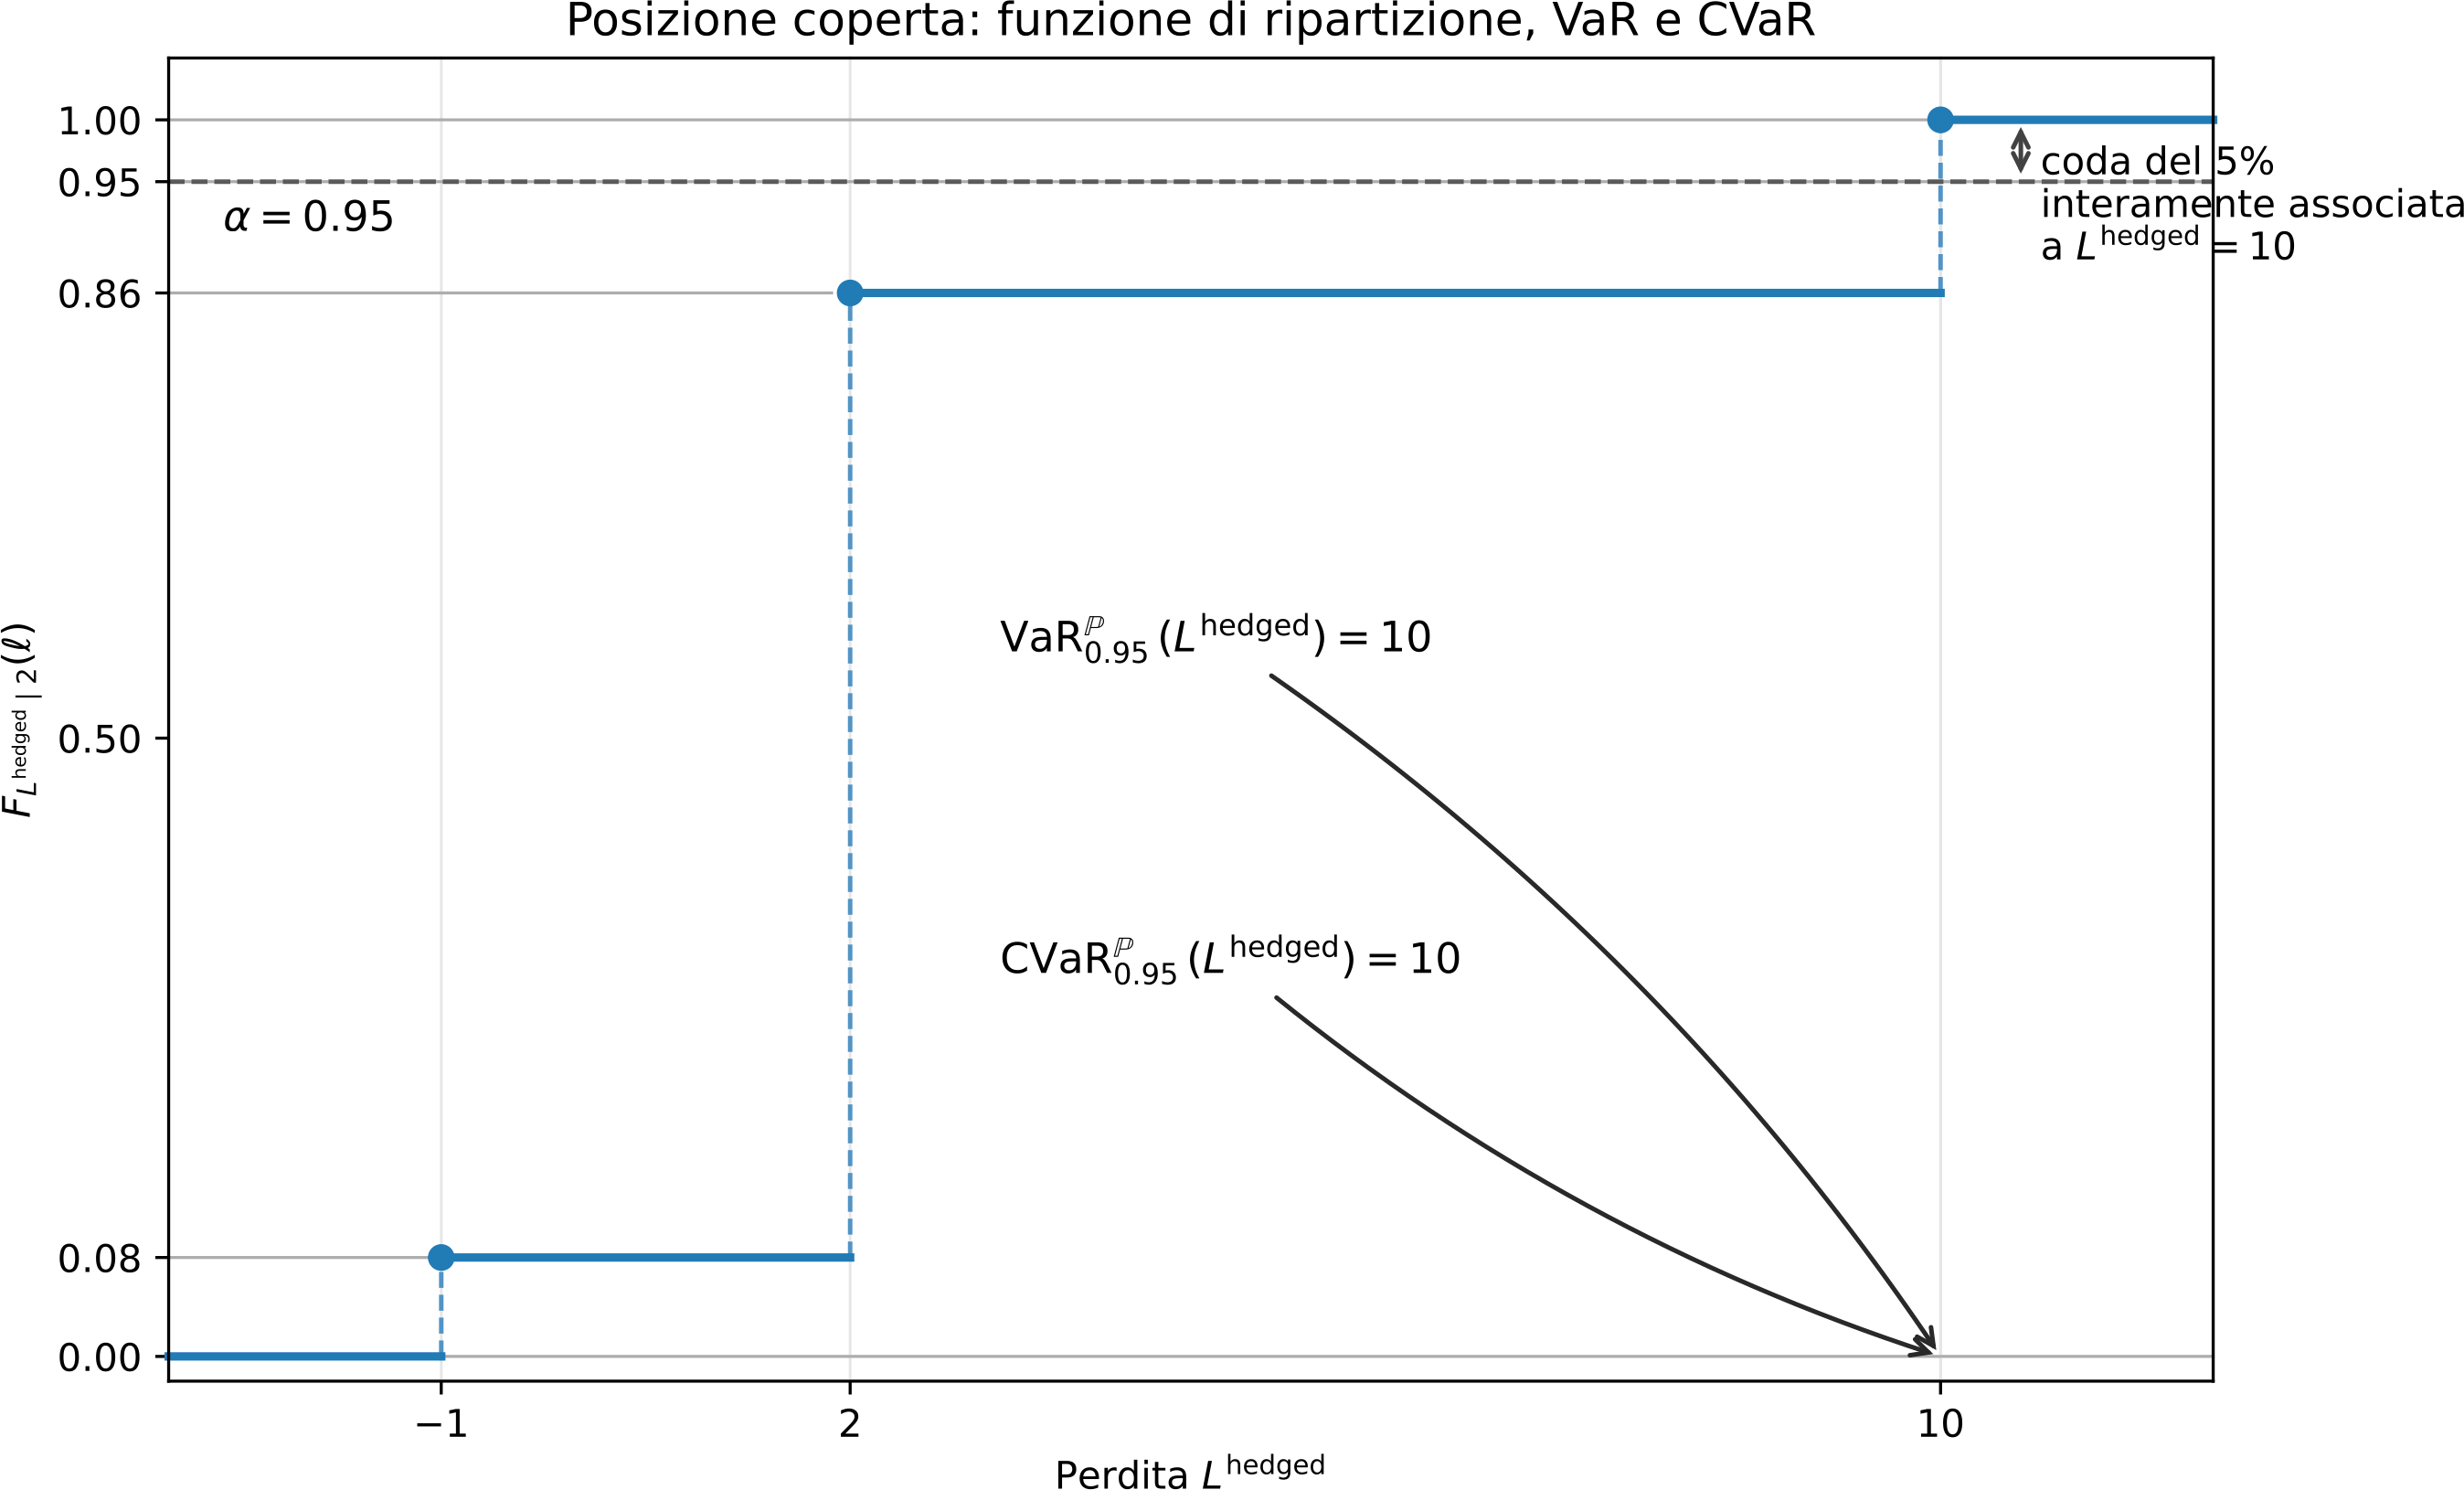
\includegraphics[width=0.82\textwidth]
{../graphics/Cap09_cdf_hedged_var_cvar.png}
\caption{Funzione di ripartizione della perdita della posizione coperta.
Al livello $\alpha=0.95$, si ha $\VaR_{0.95}^{\Prob}(L^{\mathrm{hedged}})=10$.
La coda peggiore di probabilit\`{a} $0.05$ \`{e} interamente contenuta
nell'atomo in corrispondenza della perdita $10$, e quindi
$\CVaR_{0.95}^{\Prob}(L^{\mathrm{hedged}})=10$.}
\label{fig:cap09-cdf-hedged-var-cvar}
\end{figure}


Il confronto complessivo \`{e}

\[
\begin{array}{lcc}
\hline
\text{misura}
&
\text{posizione non coperta}
&
\text{posizione coperta}
\\
\hline
\E^{\Prob}[L]
&
2.68
&
2.88
\\
\VaR_{0.95}^{\Prob}(L)
&
8
&
10
\\
\CVaR_{0.95}^{\Prob}(L)
&
39.2
&
10
\\
\hline
\end{array}
\]

La copertura riduce fortemente il CVaR, poich\'{e} elimina la perdita
estrema da default. Nello stesso esempio, tuttavia, la perdita attesa
aumenta da $2.68$ a $2.88$, poich\'{e}

\[
C^{\mathrm{premi}}
=
2
>
1.80
=
\E^{\Prob}
\left[
\Pi^{\mathrm{CDS}}
\right].
\]

Anche il VaR aumenta, passando da $8$ a $10$. Il premio certo sposta
infatti verso destra le perdite negli stati non-default e porta la
perdita da downgrade da $8$ a $10$.

Non vi \`{e} contraddizione tra questi risultati. Il CDS modifica la
forma dell'intera distribuzione: pu\`{o} ridurre la severit\`{a} della
coda estrema e, contemporaneamente, aumentare la perdita media o un
determinato quantile.

Il costo $2$ non deve essere interpretato come valore atteso fisico
della protezione. Il premio contrattuale viene determinato sotto la
misura risk-neutral, mentre le misure di rischio della posizione
coperta sono calcolate sotto la misura fisica.

\subsection{Limiti della copertura}

\label{subsec:cap9-limiti-copertura-cds}

La riduzione del rischio ottenuta mediante un CDS dipende dalla
corrispondenza tra il contratto di protezione e l'esposizione
sottostante.

\paragraph{Basis risk.}

Il valore dell'esposizione e quello del CDS possono reagire in modo
differente alle variazioni del merito creditizio, della liquidit\`{a}
e delle condizioni di mercato. Il differenziale tra lo spread
dell'obbligazione e lo spread del CDS pu\`{o} quindi variare nel tempo.
La copertura basata sul CDS non replica necessariamente in modo esatto
le variazioni di valore dell'esposizione.

\paragraph{Mismatch di nozionale.}

Se il nozionale del CDS differisce dall'esposizione effettiva, il
pagamento di protezione pu\`{o} essere insufficiente oppure eccedere la
perdita creditizia. Nel primo caso rimane una quota di rischio non
coperta; nel secondo si determina una posizione sovracoperta.

\paragraph{Mismatch di scadenza.}

La scadenza del CDS pu\`{o} essere anteriore o posteriore rispetto a
quella dell'esposizione. Se la protezione termina prima
dell'esposizione, il rischio di default riemerge dopo la scadenza del
CDS. Se la protezione ha durata superiore, possono essere sostenuti
premi relativi a un periodo nel quale l'esposizione non \`{e} pi\`{u}
presente.

\paragraph{Perdite da migrazione.}

Nella formulazione basata sul solo pagamento al credit event, il CDS
non effettua alcun pagamento in seguito a un semplice downgrade. La
perdita mark-to-market dell'obbligazione pu\`{o} quindi rimanere
scoperta.

In una valutazione mark-to-market, il valore del CDS tende a crescere
quando peggiora la qualit\`{a} creditizia della reference entity e
pu\`{o} compensare parzialmente la perdita dell'obbligazione. La
compensazione non \`{e} tuttavia necessariamente completa, a causa del
basis risk, della diversa scadenza e della diversa sensibilit\`{a}
degli strumenti agli spread.

\paragraph{Rischio di controparte.}

La protezione \`{e} efficace soltanto se il protection seller \`{e} in
grado di effettuare il pagamento previsto dal contratto. Il default o
il deterioramento della controparte pu\`{o} ridurre il valore della
copertura proprio negli scenari nei quali la protezione risulta
necessaria.

\paragraph{Evento economico ed evento contrattuale.}

Un grave deterioramento economico dell'emittente non coincide
necessariamente con un credit event riconosciuto dal contratto. Il
pagamento del CDS dipende dalla definizione giuridica e contrattuale
dell'evento creditizio, non dalla sola presenza di una perdita
economica sull'esposizione.

La qualit\`{a} della copertura deve quindi essere valutata confrontando
le distribuzioni complete delle due posizioni:

\[
L^{\mathrm{unhedged}}
\qquad
\text{e}
\qquad
L^{\mathrm{hedged}}.
\]

Una riduzione del CVaR non implica necessariamente una riduzione della
perdita attesa o del VaR. Le differenti misure descrivono aspetti
diversi della distribuzione e possono muoversi in direzioni opposte
quando il pagamento di protezione elimina gli eventi estremi, mentre
il costo dei premi incide su tutti o su molti degli altri stati.

\section{Dal singolo emittente al portafoglio}

\label{sec:cap9-portafoglio}

Le sezioni precedenti hanno considerato il rischio di una singola
esposizione. Un portafoglio creditizio contiene invece numerosi
emittenti, eventualmente caratterizzati da rating iniziali,
esposizioni, recovery rate e matrici di transizione differenti.

Il passaggio dal singolo emittente al portafoglio non consiste nella
sola somma delle probabilit\`{a} marginali. Occorre specificare anche
come le migrazioni dei rating e i default dei differenti emittenti
dipendano tra loro.

Salvo diversa indicazione, in questa sezione le probabilit\`{a} e le
misure di rischio sono considerate sotto la misura fisica $\Prob$.

\subsection{Perdita aggregata}

\label{subsec:cap9-perdita-portafoglio}

Consideriamo un portafoglio formato da $N$ esposizioni. Per
l'esposizione $n$, indichiamo con $X_{n,h}$ il rating alla data $h$ e
con

\[
L_{n,h}
=
\ell_n(X_{n,h},h)
\]

la corrispondente perdita.

La funzione $\ell_n$ pu\`{o} dipendere dalle caratteristiche
specifiche dell'esposizione, tra le quali:

\[
\mathrm{EAD}_{n,h},
\qquad
\mathrm{LGD}_{n,h},
\qquad
\text{scadenza},
\qquad
\text{struttura dei flussi}.
\]

Nel modello default-only, ad esempio,

\[
L_{n,h}
=
\mathrm{EAD}_{n,h}
\mathrm{LGD}_{n,h}
\1_{\{\tau_{D,n}\leq h\}},
\]

dove $\tau_{D,n}$ indica il tempo di default dell'emittente $n$.

Nel modello basato sulle migrazioni del rating, invece,

\[
L_{n,h}
=
V_n^{\mathrm{ref}}(h)
-
V_{n,X_{n,h}}(h),
\]

cosicch\'{e} la perdita pu\`{o} essere generata anche da un downgrade
che non determina il default.

La perdita aggregata del portafoglio all'orizzonte $h$ \`{e}

\[
L_h^{\mathrm{port}}
=
\sum_{n=1}^{N}
L_{n,h}.
\]

Per linearit\`{a} del valore atteso,

\[
\E^{\Prob}
\left[
L_h^{\mathrm{port}}
\right]
=
\sum_{n=1}^{N}
\E^{\Prob}
\left[
L_{n,h}
\right].
\]

Questa relazione vale indipendentemente dalla struttura di dipendenza
tra le esposizioni. Per calcolare la perdita attesa del portafoglio
sono quindi sufficienti le distribuzioni marginali delle singole
perdite.

La varianza della perdita aggregata \`{e} invece

\[
\begin{split}
\Var^{\Prob}
\left(
L_h^{\mathrm{port}}
\right)
&=
\sum_{n=1}^{N}
\Var^{\Prob}(L_{n,h})
\\
&\quad
+
2
\sum_{n=1}^{N-1}
\sum_{m=n+1}^{N}
\Cov^{\Prob}(L_{n,h},L_{m,h}).
\end{split}
\]

Le covarianze mostrano che la dispersione della perdita di portafoglio
dipende dal modo in cui le perdite individuali tendono a verificarsi
congiuntamente.

La dipendenza diventa ancora pi\`{u} importante per il VaR e il CVaR,
che dipendono dalla forma complessiva della distribuzione aggregata e
non possono essere ricavati sommando le corrispondenti misure
marginali.

In generale,

\[
\VaR_{\alpha}^{\Prob}
\left(
\sum_{n=1}^{N}L_{n,h}
\right)
\neq
\sum_{n=1}^{N}
\VaR_{\alpha}^{\Prob}(L_{n,h}),
\]

e analogamente il CVaR del portafoglio deve essere calcolato sulla
distribuzione di $L_h^{\mathrm{port}}$.

\subsection{Distribuzioni marginali e distribuzione congiunta}

\label{subsec:cap9-marginali-congiunta}

Per ciascun emittente $n=1,...,N$, la matrice di transizione
$P_n^{\Prob}$ determina la distribuzione del suo rating futuro. Se
l'emittente parte dal rating $i_n$, si ha

\[
\Prob
\left(
X_{n,h}=j
\mid
X_{n,0}=i_n
\right)
=
\left[
\left(P_n^{\Prob}\right)^h
\right]_{i_nj}.
\]

Queste probabilit\`{a} descrivono il comportamento del singolo
emittente considerato separatamente dagli altri. Esse costituiscono la
distribuzione marginale del rating $X_{n,h}$.

Attraverso la funzione di perdita $\ell_n$, dalla distribuzione del
rating si ricava la distribuzione marginale della perdita individuale

\[
L_{n,h}
=
\ell_n(X_{n,h},h).
\]

Per ciascun emittente $n$, la matrice di transizione
$P_n^{\Prob}$ determina la distribuzione del rating futuro,
condizionatamente al rating iniziale dell'emittente stesso:

\[
\Prob
\left(
X_{n,h}=j
\mid
X_{n,0}=i_n
\right)
=
\left[
\left(P_n^{\Prob}\right)^h
\right]_{i_nj}.
\]

Queste probabilit\`{a} descrivono separatamente i possibili rating
futuri di ciascun emittente. Esse determinano quindi le distribuzioni
individuali delle variabili

\[
X_{1,h},
X_{2,h},
\ldots,
X_{N,h}.
\]

Per rappresentare congiuntamente i rating futuri dell'intero
portafoglio introduciamo il vettore

\[
\mathbf{X}_h
=
\left(
X_{1,h},
X_{2,h},
\ldots,
X_{N,h}
\right),
\]

e il corrispondente vettore dei rating iniziali

\[
\mathbf{X}_0
=
\left(
X_{1,0},
X_{2,0},
\ldots,
X_{N,0}
\right).
\]

Rispetto al vettore $\mathbf{X}_h$, le distribuzioni individuali dei
singoli rating sono dette \emph{distribuzioni marginali}. Esse
indicano le probabilit\`{a} dei possibili rating futuri di ciascun
emittente considerato separatamente, ma non specificano con quali
probabilit\`{a} tali rating si realizzino simultaneamente.

Per descrivere le realizzazioni simultanee occorre invece conoscere la
distribuzione congiunta del vettore $\mathbf{X}_h$. Essa assegna una
probabilit\`{a} a ogni possibile configurazione dei rating futuri:

\[
\begin{split}
&
\Prob
\left(
\mathbf{X}_h=(j_1,\ldots,j_N)
\mid
\mathbf{X}_0=(i_1,\ldots,i_N)
\right)
\\
&=
\Prob
\left(
X_{1,h}=j_1,
\ldots,
X_{N,h}=j_N
\mid
X_{1,0}=i_1,
\ldots,
X_{N,0}=i_N
\right).
\end{split}
\]

La distribuzione congiunta \`{e} necessaria per determinare la
distribuzione della perdita aggregata

\[
L_h^{\mathrm{port}}
=
\sum_{n=1}^{N}
\ell_n(X_{n,h},h).
\]

Le matrici di transizione dei singoli emittenti determinano dunque le
distribuzioni marginali dei rating e delle corrispondenti perdite, ma
non determinano la distribuzione congiunta delle loro realizzazioni e,
di conseguenza, non sono sufficienti per ricavare la distribuzione
della perdita di portafoglio.

La relazione fondamentale \`{e}

\[
\boxed{
\begin{array}{c}
\text{matrici di transizione dei singoli emittenti}
\\[1mm]
\downarrow
\\[1mm]
\text{distribuzioni individuali dei rating}
\\
\text{e delle corrispondenti perdite}
\\[3mm]
\not\Longrightarrow
\\[3mm]
\text{distribuzione della perdita aggregata}
\end{array}
}
\]


Soltanto assumendo indipendenza tra le migrazioni si potrebbe scrivere

\[
\begin{split}
&
\Prob
\left(
X_{1,h}=j_1,\ldots,X_{N,h}=j_N
\mid
\mathbf{X}_0=\mathbf{i}
\right)
\\
&=
\prod_{n=1}^{N}
\Prob
\left(
X_{n,h}=j_n
\mid
X_{n,0}=i_n
\right).
\end{split}
\]

L'indipendenza costituisce tuttavia un'ipotesi particolarmente forte, e nella pratica poco realistica.
Durante una recessione, una crisi settoriale o uno shock finanziario,
pi\`{u} emittenti possono subire simultaneamente downgrade o default.

\begin{example}

Consideriamo un portafoglio formato da due emittenti. Il vettore dei
rating iniziali \`{e}

\[
\mathbf{X}_0
=
\left(
X_{1,0},
X_{2,0}
\right).
\]

Supponiamo che entrambi gli emittenti appartengano inizialmente alla
classe di rating $2$:

\[
\mathbf{X}_0
=
\mathbf{i}
=
(2,2).
\]

All'orizzonte $h$, ciascun emittente pu\`{o} soltanto permanere nello
stato $2$ oppure entrare nello stato di default $D$:

\[
X_{1,h},X_{2,h}
\in
\{2,D\}.
\]

Il vettore dei rating futuri \`{e}

\[
\mathbf{X}_h
=
\left(
X_{1,h},
X_{2,h}
\right).
\]

Le sue possibili realizzazioni sono

\[
\mathbf{j}
\in
\{
(2,2),
(D,2),
(2,D),
(D,D)
\}.
\]

Per la configurazione iniziale fissata $\mathbf{i}=(2,2)$, indichiamo
con

\[
p_h(\mathbf{i},\mathbf{j})
=
\Prob
\left(
\mathbf{X}_h=\mathbf{j}
\mid
\mathbf{X}_0=\mathbf{i}
\right)
\]

la probabilit\`{a} della configurazione futura $\mathbf{j}$.

Al variare di $\mathbf{j}$, le quantit\`{a}
$p_h(\mathbf{i},\mathbf{j})$ costituiscono la distribuzione congiunta
dei rating futuri, condizionata alla configurazione iniziale
$\mathbf{i}$.

Supponiamo che entrambi gli emittenti abbiano probabilit\`{a}
individuale di default pari a $0.05$:

\[
\Prob
\left(
X_{1,h}=D
\mid
\mathbf{X}_0=\mathbf{i}
\right)
=
\Prob
\left(
X_{2,h}=D
\mid
\mathbf{X}_0=\mathbf{i}
\right)
=
0.05.
\]

Le corrispondenti probabilit\`{a} di permanenza nello stato $2$ sono
pari a $0.95$. Confronteremo due diverse distribuzioni congiunte,
entrambe compatibili con queste stesse distribuzioni marginali.

\paragraph{Primo modello: default indipendenti.}

Se i rating futuri dei due emittenti sono indipendenti,
condizionatamente alla configurazione iniziale, la distribuzione
congiunta \`{e}

\[
\begin{array}{c|cc|c}
&
X_{2,h}=2
&
X_{2,h}=D
&
\text{totale}
\\
\hline
X_{1,h}=2
&
0.9025
&
0.0475
&
0.95
\\
X_{1,h}=D
&
0.0475
&
0.0025
&
0.05
\\
\hline
\text{totale}
&
0.95
&
0.05
&
1
\end{array}
\]

Le somme di riga forniscono la distribuzione marginale di $X_{1,h}$,
mentre le somme di colonna forniscono la distribuzione marginale di
$X_{2,h}$.

In particolare,

\[
\Prob
\left(
X_{1,h}=D
\mid
\mathbf{X}_0=\mathbf{i}
\right)
=
0.0475+0.0025
=
0.05,
\]

e

\[
\Prob
\left(
X_{2,h}=D
\mid
\mathbf{X}_0=\mathbf{i}
\right)
=
0.0475+0.0025
=
0.05.
\]

La probabilit\`{a} congiunta del doppio default \`{e}

\[
\Prob
\left(
X_{1,h}=D,
X_{2,h}=D
\mid
\mathbf{X}_0=\mathbf{i}
\right)
=
0.0025.
\]

\paragraph{Secondo modello: default perfettamente dipendenti.}

Supponiamo ora che i due emittenti subiscano sempre il default
congiuntamente. La distribuzione congiunta diventa

\[
\begin{array}{c|cc|c}
&
X_{2,h}=2
&
X_{2,h}=D
&
\text{totale}
\\
\hline
X_{1,h}=2
&
0.95
&
0
&
0.95
\\
X_{1,h}=D
&
0
&
0.05
&
0.05
\\
\hline
\text{totale}
&
0.95
&
0.05
&
1
\end{array}
\]

Le probabilit\`{a} marginali sono rimaste invariate:

\[
\Prob
\left(
X_{1,h}=D
\mid
\mathbf{X}_0=\mathbf{i}
\right)
=
0.05,
\]

e

\[
\Prob
\left(
X_{2,h}=D
\mid
\mathbf{X}_0=\mathbf{i}
\right)
=
0.05.
\]

La probabilit\`{a} congiunta del doppio default \`{e} invece

\[
\Prob
\left(
X_{1,h}=D,
X_{2,h}=D
\mid
\mathbf{X}_0=\mathbf{i}
\right)
=
0.05.
\]

Le due distribuzioni congiunte hanno pertanto gli stessi margini, ma
attribuiscono probabilit\`{a} differenti alle realizzazioni
simultanee:

\[
\begin{array}{c|cc}
&
\text{indipendenza}
&
\text{dipendenza perfetta}
\\
\hline
\Prob
\left(
X_{1,h}=D,
X_{2,h}=D
\mid
\mathbf{X}_0=\mathbf{i}
\right)
&
0.0025
&
0.05
\end{array}
\]

Supponiamo infine che ciascuna esposizione produca una perdita unitaria
in caso di default:

\[
L_{1,h}
=
\1_{\{X_{1,h}=D\}},
\qquad
L_{2,h}
=
\1_{\{X_{2,h}=D\}}.
\]

La perdita aggregata \`{e}

\[
L_h^{\mathrm{port}}
=
L_{1,h}+L_{2,h}.
\]

La corrispondenza tra configurazioni dei rating e perdita aggregata
\`{e}

\[
\begin{array}{c|cccc}
\mathbf{X}_h
&
(2,2)
&
(D,2)
&
(2,D)
&
(D,D)
\\
\hline
L_h^{\mathrm{port}}
&
0
&
1
&
1
&
2
\end{array}
\]

Nel modello con default indipendenti si ottiene

\[
\begin{array}{c|ccc}
L_h^{\mathrm{port}}
&
0
&
1
&
2
\\
\hline
\Prob
\left(
L_h^{\mathrm{port}}=\ell
\mid
\mathbf{X}_0=\mathbf{i}
\right)
&
0.9025
&
0.0950
&
0.0025
\end{array}
\]

Nel modello con default perfettamente dipendenti si ottiene invece

\[
\begin{array}{c|ccc}
L_h^{\mathrm{port}}
&
0
&
1
&
2
\\
\hline
\Prob
\left(
L_h^{\mathrm{port}}=\ell
\mid
\mathbf{X}_0=\mathbf{i}
\right)
&
0.95
&
0
&
0.05
\end{array}
\]

Le distribuzioni marginali dei rating individuali sono identiche nei
due modelli. La diversa struttura di dipendenza modifica tuttavia la
distribuzione congiunta dei rating e, di conseguenza, la distribuzione
della perdita aggregata.

\end{example}

\subsection{Concentrazione e fattori comuni}

\label{subsec:cap9-concentrazione-fattori}

La dipendenza tra le perdite pu\`{o} derivare da fattori economici
comuni e dalla composizione del portafoglio.

\paragraph{Concentrazione per debitore.}

Un portafoglio \`{e} concentrato per debitore quando una parte
rilevante dell'esposizione complessiva dipende da pochi emittenti. Se

\[
w_n
=
\frac{
\mathrm{EAD}_{n,h}
}{
\displaystyle
\sum_{m=1}^{N}
\mathrm{EAD}_{m,h}
},
\]

un valore elevato di $w_n$ indica che il deterioramento del debitore
$n$ pu\`{o} produrre una quota rilevante della perdita totale.

La presenza di molti emittenti non garantisce quindi
automaticamente una diversificazione effettiva, se il portafoglio
rimane dominato da poche esposizioni di grandi dimensioni.

\paragraph{Concentrazione settoriale.}

Emittenti appartenenti allo stesso settore possono reagire in modo
simile a variazioni dei prezzi delle materie prime, dei tassi di
interesse, della domanda o della regolamentazione.

Un portafoglio composto da numerosi debitori dello stesso settore pu\`{o}
essere poco diversificato, anche quando nessuna singola esposizione
risulta dominante.

\paragraph{Concentrazione geografica.}

La localizzazione degli emittenti in una stessa area economica espone
il portafoglio a shock comuni relativi alla crescita, alla politica
fiscale, al sistema bancario, al rischio sovrano o al quadro
istituzionale.

La diversificazione per numero di debitori pu\`{o} quindi essere
inefficace se le esposizioni rimangono concentrate nella stessa
economia.

\paragraph{Dipendenza macroeconomica.}

Le probabilit\`{a} di transizione possono dipendere da un fattore
macroeconomico comune $Z_h$, ad esempio uno stato di espansione,
rallentamento o recessione.

Condizionatamente a $Z_h$, le transizioni individuali possono essere
modellate come indipendenti:

\[
\begin{split}
&
\Prob
\left(
X_{1,h}=j_1,\ldots,X_{N,h}=j_N
\mid
Z_h,\mathbf{X}_0
\right)
\\
&=
\prod_{n=1}^{N}
\Prob
\left(
X_{n,h}=j_n
\mid
Z_h,X_{n,0}
\right).
\end{split}
\]

Senza condizionare sul fattore comune, le migrazioni risultano invece
dipendenti. Uno stato macroeconomico sfavorevole aumenta
simultaneamente la probabilit\`{a} di downgrade e default di numerosi
emittenti.

\paragraph{Default clustering.}

Con l'espressione \emph{default clustering} si indica la tendenza dei
default a concentrarsi negli stessi periodi anzich\'{e} distribuirsi
uniformemente nel tempo.

Il fenomeno pu\`{o} derivare da recessioni, crisi di liquidit\`{a},
shock settoriali, legami commerciali o esposizioni comuni alle stesse
fonti di finanziamento.

Il clustering aumenta la probabilit\`{a} di perdite aggregate molto
elevate e incide soprattutto sulla parte estrema della distribuzione.
Per questo motivo, trascurare la dipendenza pu\`{o} produrre una
sottostima significativa del VaR e del CVaR di portafoglio.

\subsection{Derivati multi-name}

\label{subsec:cap9-derivati-multiname}

Il CDS analizzato nelle sezioni precedenti \`{e} riferito a una singola
reference entity. Esistono anche derivati di credito il cui payoff
dipende da pi\`{u} emittenti.

Tra i principali strumenti multi-name rientrano:

\begin{itemize}

\item i \emph{CDS index}, riferiti a un insieme standardizzato di
emittenti;

\item i \emph{basket CDS}, riferiti a un paniere di debitori
specificamente selezionato;

\item i contratti \emph{first-to-default}, nei quali la protezione
viene attivata dal primo default all'interno del paniere;

\item le tranche creditizie, il cui payoff dipende dalla perdita
aggregata del portafoglio compresa tra determinati livelli di
assorbimento.

\end{itemize}

Nel contratto first-to-default, il tempo rilevante \`{e}

\[
\tau_{(1)}
=
\min
\{
\tau_{D,1},
\ldots,
\tau_{D,N}
\}.
\]

La probabilit\`{a} che il contratto venga attivato entro l'orizzonte
$H$ \`{e}

\[
\Prob(\tau_{(1)}\leq H).
\]

Questa probabilit\`{a} non pu\`{o} essere determinata conoscendo
soltanto le probabilit\`{a} marginali

\[
\Prob(\tau_{D,n}\leq H).
\]

Occorre specificare la dipendenza tra i tempi di default.

\begin{definition}
Una \emph{tranche creditizia} \`{e} una porzione contrattualmente
definita della perdita aggregata di un portafoglio. Essa \`{e}
identificata da due livelli

\[
0\leq A<B,
\]

dove $A$ \`{e} l'\emph{attachment point} e $B$ il
\emph{detachment point}.
\end{definition}

Indicando con $L_h^{\mathrm{port}}$ la perdita aggregata del
portafoglio, la perdita assorbita dalla tranche pu\`{o} essere
rappresentata come

\[
L_h^{\mathrm{tr}}(A,B)
=
\left(
L_h^{\mathrm{port}}-A
\right)^{+}
-
\left(
L_h^{\mathrm{port}}-B
\right)^{+}.
\]

Equivalentemente,

\[
L_h^{\mathrm{tr}}(A,B)
=
\min
\left\{
\left(
L_h^{\mathrm{port}}-A
\right)^{+},
B-A
\right\}.
\]Indicando con $L_h^{\mathrm{port}}$ la perdita aggregata del
portafoglio, la perdita assorbita dalla tranche pu\`{o} essere
rappresentata come

\[
L_h^{\mathrm{tr}}(A,B)
=
\left(
L_h^{\mathrm{port}}-A
\right)^{+}
-
\left(
L_h^{\mathrm{port}}-B
\right)^{+}.
\]

Equivalentemente,

\[
L_h^{\mathrm{tr}}(A,B)
=
\min
\left\{
\left(
L_h^{\mathrm{port}}-A
\right)^{+},
B-A
\right\}.
\]

La Figura~\ref{fig:cap09-tranche-creditizia} mostra come la perdita
della tranche dipenda dalla perdita aggregata del portafoglio.

\begin{figure}[htbp]
\centering
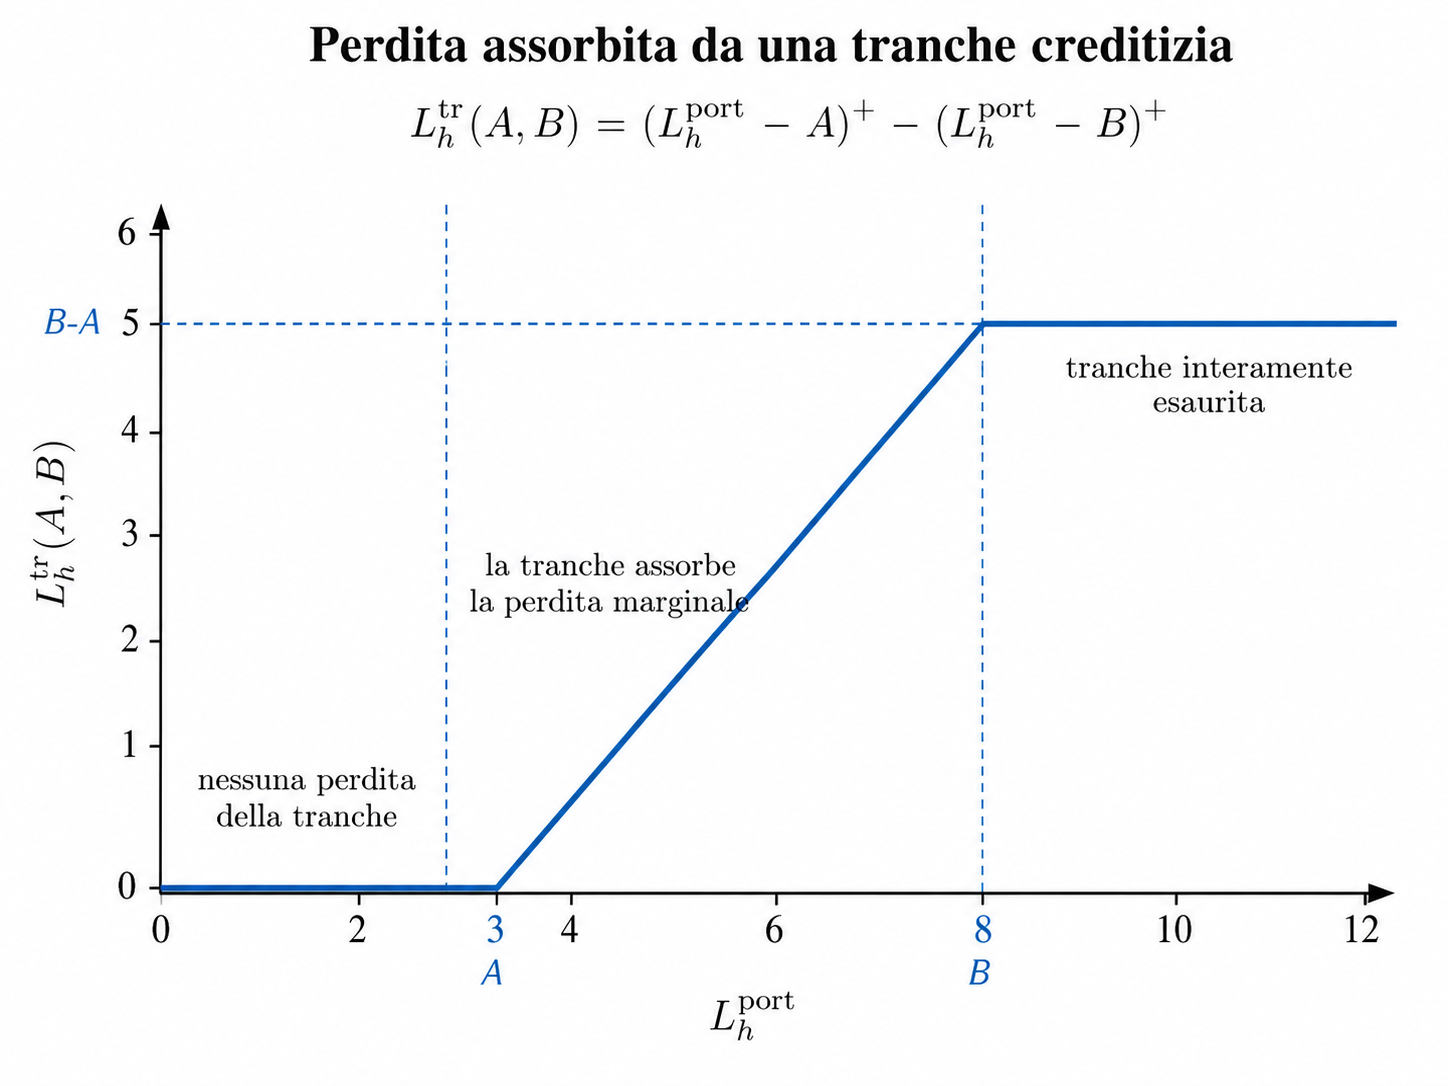
\includegraphics[width=0.82\textwidth]
{../graphics/Cap09_tranche_creditizia.png}
\caption{Profilo della perdita assorbita da una tranche creditizia con
attachment point $A$ e detachment point $B$.}
\label{fig:cap09-tranche-creditizia}
\end{figure}

La tranche non subisce perdite finch\'{e}

\[
L_h^{\mathrm{port}}\leq A.
\]

Per

\[
A<L_h^{\mathrm{port}}<B,
\]

la perdita della tranche cresce nella stessa misura della perdita
aggregata eccedente l'attachment point. Infine, quando

\[
L_h^{\mathrm{port}}\geq B,
\]

la tranche risulta interamente esaurita e la sua perdita raggiunge il
valore massimo

\[
B-A.
\]



La tranche non subisce perdite finch\'{e} la perdita aggregata rimane
inferiore ad $A$. Assorbe le perdite comprese tra $A$ e $B$ ed
\`{e} interamente esaurita quando

\[
L_h^{\mathrm{port}}\geq B.
\]

Per descrivere i flussi associati alla tranche occorre quindi
conoscere la distribuzione della perdita aggregata del portafoglio.
La dipendenza tra i default, influenzando la frequenza e la
concentrazione delle perdite elevate, diventa pertanto un elemento
essenziale.

Il pricing dei derivati multi-name non viene sviluppato nel presente
corso. Questi strumenti mostrano tuttavia perch\'{e} la modellizzazione
della dipendenza sia indispensabile: lo stesso insieme di probabilit\`{a}
marginali pu\`{o} generare valori e distribuzioni di perdita molto
differenti al variare della struttura congiunta.

\subsection{Raccordo con la Lezione 10}

\label{subsec:cap9-raccordo-lezione10}

Per un portafoglio con molti emittenti, la costruzione analitica della
distribuzione congiunta pu\`{o} diventare rapidamente complessa. La
Lezione~10 utilizzer\`{a} la simulazione per generare scenari congiunti
dei rating e delle perdite.

La struttura dell'applicazione sar\`{a}

\[
\boxed{
\begin{array}{c}
\text{transizioni individuali}
\\
+
\\
\text{dipendenza e fattori comuni}
\\
+
\\
\mathrm{LGD}\text{ ed }\mathrm{EAD}
\\
\downarrow
\\
\text{distribuzione simulata della perdita di portafoglio}.
\end{array}
}
\]

In ciascuno scenario simulato si proceder\`{a} a:

\begin{enumerate}

\item generare lo stato del fattore macroeconomico comune;

\item simulare le transizioni dei singoli emittenti condizionatamente
al fattore comune e ai rating iniziali;

\item associare a ogni stato futuro una perdita dipendente da
$\mathrm{LGD}$, $\mathrm{EAD}$ e dalla variazione di valore
dell'esposizione;

\item aggregare le perdite individuali:

\[
L_h^{\mathrm{port}}
=
\sum_{n=1}^{N}L_{n,h};
\]

\item ripetere la simulazione per ottenere una distribuzione empirica
della perdita aggregata;

\item stimare perdita attesa, varianza, VaR e CVaR del portafoglio.

\end{enumerate}

La Lezione~10 mostrer\`{a} quindi il passaggio operativo dalle matrici
marginali di transizione a una distribuzione di portafoglio nella quale
la dipendenza viene specificata e simulata esplicitamente.

\section{Impiego gestionale e regolamentare delle misure}

\label{sec:cap9-impiego-gestionale-regolamentare}

Le misure introdotte nel capitolo trovano applicazione nella gestione
del rischio, nella redazione del bilancio e nella valutazione
dell'adeguatezza patrimoniale. I diversi ambiti utilizzano concetti
collegati, ma non coincidenti.

In particolare, occorre distinguere tra:

\begin{itemize}
\item la perdita attesa;
\item gli accantonamenti contabili;
\item il capitale economico;
\item i requisiti patrimoniali prudenziali.
\end{itemize}

La presente sezione fornisce soltanto un inquadramento professionale.
La disciplina contabile e prudenziale completa viene rinviata agli
insegnamenti specialistici.

\subsection{Accantonamenti e IFRS 9}

\label{subsec:cap9-ifrs9}

Il principio contabile IFRS~9 adotta un modello fondato sulle
\emph{expected credit losses}, indicate con ECL. L'accantonamento
contabile dipende dall'evoluzione del rischio creditizio dello
strumento rispetto alla data della sua rilevazione iniziale.

L'IFRS~9 distingue due basi di misurazione delle perdite attese:

\begin{itemize}

\item l'\emph{expected credit loss a 12 mesi};

\item la \emph{lifetime expected credit loss}.

\end{itemize}

La differenza riguarda l'orizzonte entro il quale pu\`{o} verificarsi
il default. L'ECL a 12 mesi considera le perdite lungo la vita residua
dello strumento generate da eventi di default possibili nei dodici
mesi successivi. La lifetime ECL considera invece le perdite generate
da tutti i default possibili durante l'intera vita residua.

Quando si verifica un incremento significativo del rischio creditizio,
l'accantonamento viene invece determinato sulla base della
\emph{lifetime expected credit loss}, che considera gli eventi di
default possibili lungo l'intera vita residua dello strumento.

In forma schematica,

\[
\begin{array}{ccl}
\text{assenza di incremento significativo}
&
\longrightarrow
&
\text{ECL a 12 mesi},
\\[2mm]
\text{incremento significativo del rischio}
&
\longrightarrow
&
\text{lifetime ECL}.
\end{array}
\]

La valutazione dell'incremento significativo del rischio creditizio
richiede il confronto tra il rischio di default alla data corrente e
quello esistente al momento della rilevazione iniziale. Non coincide
quindi con la sola osservazione del rating corrente o con il
verificarsi del default.

Il modello markoviano sviluppato nel capitolo consente di rappresentare
in modo semplificato il collegamento tra transizioni dei rating e
lifetime ECL. Utilizzando una matrice di transizione predittiva
$P^{\Prob}$, le probabilit\`{a} marginali di default sono

\[
\mathrm{PD}_{i}^{\mathrm{marg}}(h)
=
\left[
\left(P^{\Prob}\right)^h
\right]_{iD}
-
\left[
\left(P^{\Prob}\right)^{h-1}
\right]_{iD}.
\]

In un modello discreto semplificato, definiamo la perdita creditizia
attualizzata lungo la vita residua come

\[
L_i^{\mathrm{life}}
=
\sum_{h=1}^{H}
d_h
\mathrm{LGD}_h
\mathrm{EAD}_h
\1_{\{\tau_D=h\}}.
\]

Se il default avviene alla data $h$, soltanto l'indicatrice
$\1_{\{\tau_D=h\}}$ assume valore uno. Se invece $\tau_D>H$, tutte le
indicatrici sono nulle e la perdita da default \`{e} pari a zero.
La lifetime expected credit loss \`{e} quindi il valore atteso della
perdita lungo la vita residua:

\[
\begin{split}
\mathrm{ECL}_{i}^{\mathrm{life}}
&=
\E^{\Prob}
\left[
L_i^{\mathrm{life}}
\mid X_0=i
\right]
\\
&=
\sum_{h=1}^{H}
d_h
\mathrm{PD}_{i}^{\mathrm{marg}}(h)
\mathrm{LGD}_h
\mathrm{EAD}_h.
\end{split}
\]
Il collegamento concettuale \`{e} quindi

\[
\boxed{
\left(P^{\Prob}\right)^h
\longrightarrow
\text{term structure delle probabilit\`{a} di default}
\longrightarrow
\text{lifetime ECL}.
}
\]

Nel modello annuale semplificato, l'ECL a 12 mesi utilizza la
probabilit\`{a} degli eventi di default che possono verificarsi nel
primo anno:

\[
\mathrm{ECL}_{i}^{12\mathrm{m}}
=
d_1
\mathrm{PD}_{i}^{\mathrm{marg}}(1)
\mathrm{LGD}_1
\mathrm{EAD}_1.
\]

Le formule precedenti costituiscono una rappresentazione didattica:
l'IFRS~9 non prescrive l'impiego di una matrice di transizione.

Nel modello qui adottato, la matrice $P^{\Prob}$ viene utilizzata per
ottenere probabilit\`{a} di default predittive. Una matrice stimata
sulle transizioni storiche pu\`{o} costituire il punto di partenza, ma
le probabilit\`{a} utilizzate nel calcolo dell'ECL devono riflettere
anche le condizioni correnti e le previsioni ragionevoli
sull'evoluzione futura dell'economia.

Si tratta pertanto di probabilit\`{a} sotto la misura fisica, finalizzate
alla previsione delle perdite, e non di probabilit\`{a} risk-neutral
utilizzate per il pricing.

\subsection{Capitale economico e capitale prudenziale}

\label{subsec:cap9-capitale-economico-prudenziale}

La perdita attesa, l'accantonamento contabile, il capitale economico
e il requisito patrimoniale prudenziale sono concetti collegati, ma
rispondono a finalit\`{a} differenti.

La \emph{perdita attesa} (\emph{Expected Loss}, \emph{EL}) \`{e} il
valore medio della variabile casuale perdita sotto la distribuzione
predittiva adottata:

\[
\mathrm{EL}
=
\E^{\Prob}[L].
\]

Essa rappresenta la perdita media associata all'esposizione o al
portafoglio nel modello considerato.

L'\emph{accantonamento contabile per perdite}
(\emph{loss allowance}) \`{e} invece l'importo rilevato in bilancio
a fronte delle perdite creditizie attese. Nell'IFRS~9 esso viene
misurato mediante le \emph{Expected Credit Losses} (\emph{ECL}),
utilizzando, a seconda dell'evoluzione del rischio creditizio, l'ECL
a 12 mesi oppure la lifetime ECL.

L'accantonamento contabile \`{e} quindi collegato alla perdita attesa,
ma non coincide necessariamente con la quantit\`{a} $\mathrm{EL}$
calcolata mediante un generico modello interno. La sua determinazione
dipende dalle regole contabili applicabili, dall'orizzonte considerato,
dall'attualizzazione e dalle informazioni previsionali utilizzate.

Il \emph{capitale economico} (\emph{Economic Capital}, \emph{EC})
\`{e} una misura gestionale interna delle risorse destinate ad
assorbire le perdite superiori alla perdita attesa, entro un
determinato orizzonte e livello di confidenza $\alpha$.

Secondo la convenzione adottata nel capitolo,

\[
\mathrm{EC}_{\alpha}
=
\VaR_{\alpha}(L)
-
\mathrm{EL},
\]

dove il \emph{Value at Risk} (\emph{VaR}) rappresenta il quantile
della perdita totale al livello di confidenza $\alpha$.

Il \emph{requisito patrimoniale prudenziale}
(\emph{prudential capital requirement}) \`{e} invece il capitale
richiesto dalle regole di vigilanza. Esso dipende, tra gli altri
elementi, dalle esposizioni, dalle ponderazioni per il rischio, dai
parametri regolamentari, dal metodo di calcolo applicato e dagli
eventuali requisiti o riserve aggiuntivi previsti dal quadro
prudenziale.

Le quattro nozioni possono essere sintetizzate come segue:

\[
\begin{array}{p{4.2cm}p{7.4cm}}
\hline
\textbf{Concetto}
&
\textbf{Funzione principale}
\\
\hline
\emph{Expected Loss} (\emph{EL})
&
misurare la perdita media prodotta dal modello probabilistico;
\\
\emph{loss allowance}
&
rilevare in bilancio le perdite creditizie attese misurate mediante
le \emph{ECL};
\\
\emph{Economic Capital} (\emph{EC})
&
determinare internamente le risorse destinate ad assorbire le perdite
superiori alla perdita attesa;
\\
\emph{prudential capital requirement}
&
determinare il capitale richiesto dalle regole di vigilanza.
\\
\hline
\end{array}
\]

La relazione

\[
\mathrm{EC}_{\alpha}
=
\VaR_{\alpha}(L)
-
\mathrm{EL}
\]

costituisce pertanto una convenzione gestionale per il calcolo del
capitale economico. Non rappresenta una formula generale per la
determinazione del requisito patrimoniale prudenziale.

\subsection{Stress testing}

\label{subsec:cap9-stress-testing}

Il VaR e il CVaR sono misure probabilistiche ricavate da una
distribuzione stimata delle perdite:

\[
F_L
\longrightarrow
\VaR_{\alpha}(L),
\qquad
\CVaR_{\alpha}(L).
\]

I risultati dipendono quindi dal modello adottato, dai dati utilizzati,
dalla struttura di dipendenza e dalle ipotesi formulate sulle
transizioni, sulle esposizioni e sui tassi di recupero.

Lo stress testing segue una logica differente. Si specifica uno
scenario avverso, ad esempio una recessione, un aumento dei default,
una riduzione dei recovery rate o un deterioramento simultaneo di
determinati settori, e si valuta la perdita che ne deriverebbe.

Indicando con $z^{\mathrm{stress}}$ lo scenario avverso assegnato, si
considera una quantit\`{a} del tipo

\[
L^{\mathrm{stress}}
=
L\left(z^{\mathrm{stress}}\right).
\]

Lo scenario di stress non deve necessariamente essere identificato
con un quantile della distribuzione stimata, n\'{e} deve essergli
attribuita una probabilit\`{a} precisa. La sua funzione \`{e} valutare
la vulnerabilit\`{a} della posizione o del portafoglio rispetto a una
configurazione avversa specifica.

Le due prospettive sono complementari:

\[
\boxed{
\begin{array}{c}
\text{misure probabilistiche}
\quad+\quad
\text{scenari di stress}
\\[-0.5mm]
\longrightarrow
\quad
\text{valutazione pi\`{u} completa del rischio}
\end{array}
}
\]

Il VaR e il CVaR sintetizzano la distribuzione prodotta dal modello; lo
stress testing verifica invece le conseguenze di scenari avversi che
possono risultare particolarmente rilevanti dal punto di vista
gestionale o prudenziale.

\section{Limiti del modello e rischio di modello}

\label{sec:cap9-limiti-rischio-modello}

Le misure di rischio ottenute nel capitolo non sono quantit\`{a}
direttamente osservabili. Esse sono il risultato di una successione di
scelte modellistiche che riguardano la dinamica dei rating, la
traduzione degli stati futuri in perdite e, nel caso di un portafoglio,
la dipendenza tra gli emittenti.

Nel presente capitolo, con \emph{rischio di modello}
(\emph{model risk}) si indica il rischio che una rappresentazione
incompleta, non adeguatamente specificata o non correttamente calibrata
produca stime delle perdite e delle misure di rischio non sufficientemente
affidabili.

I limiti del modello vengono quindi organizzati secondo le principali
componenti della catena di misurazione.

\subsection{Modello delle transizioni}

\label{subsec:cap9-limiti-transizioni}

Il modello delle transizioni determina le probabilit\`{a} associate ai
rating futuri e al default. Le sue conclusioni dipendono dalla validit\`{a}
della struttura markoviana e dalla capacit\`{a} della matrice di
transizione di rappresentare l'evoluzione futura del rischio creditizio.

\paragraph{Validit\`{a} della propriet\`{a} di Markov.}

La propriet\`{a} di Markov assume che, condizionatamente al rating
corrente, la distribuzione del rating futuro non dipenda ulteriormente
dalla storia precedente dell'emittente.

Questa ipotesi pu\`{o} risultare restrittiva. Due emittenti collocati
nella stessa classe di rating possono avere prospettive differenti se
uno vi permane da diversi anni, mentre l'altro vi \`{e} appena entrato
in seguito a un downgrade. La durata della permanenza nello stato, la
direzione delle precedenti migrazioni e altre informazioni storiche
possono quindi contenere capacit\`{a} predittiva non rappresentata dal
solo rating corrente.

In questi casi, il modello pu\`{o} essere ampliato introducendo ulteriori
variabili di stato oppure adottando una dinamica non strettamente
markoviana.

\paragraph{Omogeneit\`{a} temporale.}

Nel modello omogeneo, una sola matrice $P$ descrive le probabilit\`{a}
di transizione in ogni periodo. La distribuzione a $h$ periodi viene
pertanto ottenuta mediante

\[
P^h.
\]

Questa rappresentazione presuppone che le probabilit\`{a} di upgrade,
downgrade e default restino costanti nel tempo. Tale ipotesi pu\`{o}
essere poco realistica quando il rischio creditizio varia con il ciclo
economico, con le condizioni finanziarie o con eventi settoriali.

Se la matrice dipende dal tempo, la probabilit\`{a} di transizione tra
le date $t$ e $t+h$ non \`{e} descritta da $P^h$, ma dal prodotto

\[
P_t P_{t+1}\cdots P_{t+h-1}.
\]

L'impiego di una matrice omogenea costituisce quindi una
semplificazione la cui adeguatezza dipende dall'orizzonte e dal
contesto applicativo.

\paragraph{Qualit\`{a} della classificazione dei rating.}

Il rating deve sintetizzare le informazioni rilevanti per prevedere
l'evoluzione del merito creditizio. Se le classi sono troppo ampie,
emittenti sostanzialmente differenti vengono trattati come se avessero
la stessa distribuzione futura.

Anche errori di classificazione, cambiamenti nei criteri di assegnazione
dei rating o differenze tra sistemi interni ed esterni modificano le
frequenze di transizione osservate. La matrice pu\`{o} quindi riflettere
non soltanto l'evoluzione del rischio degli emittenti, ma anche le
caratteristiche del sistema di classificazione utilizzato.

\paragraph{Rotture strutturali.}

Una matrice stimata sui dati passati pu\`{o} perdere capacit\`{a}
predittiva quando cambiano stabilmente le condizioni economiche o
istituzionali. Crisi finanziarie, modifiche normative, innovazioni nei
processi di concessione del credito o trasformazioni strutturali di un
settore possono produrre probabilit\`{a} di transizione differenti da
quelle osservate nel campione storico.

L'uso meccanico di una matrice storica presuppone quindi una stabilit\`{a}
che deve essere valutata e non semplicemente assunta.

\subsection{Modello delle perdite}

\label{subsec:cap9-limiti-perdite}

La matrice di transizione assegna probabilit\`{a} agli stati futuri,
ma non determina da sola la distribuzione delle perdite. Occorre anche
specificare la funzione di perdita

\[
\ell(j,h),
\]

che associa a ciascuno stato futuro $j$ la corrispondente conseguenza
economica. Come definito in precedenza,

\[
L_h=\ell(X_h,h).
\]

Nel modello mark-to-market adottato nel capitolo, tale funzione viene
costruita confrontando il valore dell'esposizione nello stato futuro
con il valore di riferimento:

\[
\ell(j,h)
=
V^{\mathrm{ref}}(h)-V_j(h).
\]

Anche questa trasformazione introduce ipotesi e fonti di rischio di
modello.

\paragraph{Incertezza dell'\emph{Exposure at Default} (\emph{EAD}).}

L'\emph{EAD} rappresenta l'esposizione esistente nel momento in cui si
verifica il default. Essa non coincide necessariamente con
l'esposizione osservata alla data iniziale.

Rimborsi, nuove erogazioni, utilizzi di linee di credito e variazioni
delle garanzie possono modificare l'importo effettivamente esposto. Il
trattamento dell'\emph{EAD} come quantit\`{a} deterministica trascura
questa fonte di incertezza.

\paragraph{Aleatoriet\`{a} della \emph{Loss Given Default} (\emph{LGD}).}

La \emph{LGD} misura la quota dell'esposizione che non viene recuperata
in caso di default. Essa dipende, tra gli altri elementi, dalle
garanzie disponibili, dal grado di subordinazione, dai tempi di
recupero e dai costi delle procedure.

Una rappresentazione semplificata pu\`{o} utilizzare un unico valore di
$\mathrm{LGD}$. In realt\`{a}, anche condizionatamente al default, la
perdita pu\`{o} essere aleatoria:

\[
L_h^{\mathrm{def}}
=
\mathrm{EAD}_h
\mathrm{LGD}_h
\1_{\{\tau_D=h\}}.
\]

La sostituzione di $\mathrm{EAD}_h$ e $\mathrm{LGD}_h$ con valori
deterministici riduce la variabilit\`{a} rappresentata dal modello e
pu\`{o} sottostimare la dispersione delle perdite.

\paragraph{Dipendenza dei recuperi dal ciclo economico.}

I tassi di recupero possono deteriorarsi proprio nelle fasi in cui
aumentano i default. Durante una recessione, il numero di attivit\`{a}
da liquidare pu\`{o} crescere, mentre il valore delle garanzie e la
capacit\`{a} del mercato di assorbirle possono diminuire.

Assumere una \emph{LGD} costante e indipendente dalle transizioni
creditizie elimina questa possibile relazione tra frequenza dei
default e severit\`{a} delle perdite.

\paragraph{Spread e valori associati ai rating.}

Nel modello mark-to-market, a ciascun rating viene associato uno spread
e, attraverso lo spread, un valore dello strumento. La relazione

\[
j
\longmapsto
s_j
\longmapsto
V_j(h)
\]

costituisce una componente autonoma del modello.

Emittenti appartenenti alla stessa classe possono presentare spread
differenti per effetto della liquidit\`{a}, della durata, del settore,
della struttura contrattuale e delle condizioni di mercato. Associare
un solo valore a ogni rating comprime questa eterogeneit\`{a} e rende
la perdita dipendente dalla specifica tabella di spread adottata.

\paragraph{Scelta del valore di riferimento.}

La perdita dipende anche dal valore di riferimento
$V^{\mathrm{ref}}(h)$. Il valore nominale, il valore contabile, il
valore iniziale e il valore che lo strumento avrebbe mantenendo il
rating corrente rispondono a domande differenti.

Due modelli che utilizzano le stesse probabilit\`{a} di transizione e
gli stessi valori futuri possono quindi produrre perdite differenti
se adottano valori di riferimento diversi. La scelta deve essere
coerente con la finalit\`{a} della misurazione e dichiarata
esplicitamente.

\subsection{Modello di portafoglio}

\label{subsec:cap9-limiti-portafoglio}

Per un portafoglio di $N$ esposizioni, la perdita aggregata \`{e}

\[
L_h^{\mathrm{port}}
=
\sum_{n=1}^{N}L_{n,h}.
\]

Le distribuzioni individuali delle perdite non sono tuttavia
sufficienti per determinare la distribuzione della somma. Occorre
specificare la dipendenza tra i rating futuri e tra i default dei
diversi emittenti.

\paragraph{Dipendenza tra debitori.}

Le matrici di transizione dei singoli emittenti determinano le
rispettive distribuzioni individuali, ma non determinano la
distribuzione congiunta del vettore dei rating futuri.

Modelli con le stesse probabilit\`{a} individuali di default possono
produrre probabilit\`{a} molto differenti di default simultanei. Di
conseguenza, possono generare distribuzioni di perdita, VaR e CVaR
sensibilmente differenti.

\paragraph{Concentrazione.}

La concentrazione nasce quando una parte rilevante del portafoglio
dipende da pochi debitori, settori, aree geografiche o tipologie di
garanzia. In questi casi, anche un singolo evento negativo pu\`{o}
produrre una perdita elevata.

Un modello che rappresenta correttamente le probabilit\`{a} di default,
ma trascura la distribuzione delle esposizioni, pu\`{o} sottovalutare il
rischio complessivo del portafoglio.

\paragraph{Fattori comuni.}

I debitori possono essere influenzati dagli stessi fattori
macroeconomici e finanziari, come crescita economica, tassi di
interesse, prezzi delle materie prime o condizioni di liquidit\`{a}.

L'introduzione di fattori comuni consente di rappresentare il fatto che
le transizioni peggiorative tendono a concentrarsi negli stessi
scenari. La specificazione e la calibrazione di tali fattori incidono
direttamente sulla probabilit\`{a} di perdite aggregate elevate.

\paragraph{Rischio sistematico.}

La diversificazione pu\`{o} ridurre la componente idiosincratica del
rischio, ma non elimina gli effetti degli shock comuni. Il rischio
sistematico produce dipendenza tra i debitori e pu\`{o} generare
concentrazioni di default proprio nelle fasi economiche avverse.

La varianza della perdita di portafoglio evidenzia il ruolo delle
covarianze:

\[
\Var
\left(
L_h^{\mathrm{port}}
\right)
=
\sum_{n=1}^{N}
\Var(L_{n,h})
+
2
\sum_{n<m}
\Cov(L_{n,h},L_{m,h}).
\]

Per le misure di coda, la sola conoscenza delle covarianze non \`{e}
generalmente sufficiente: assumono rilievo anche la forma della
dipendenza e la probabilit\`{a} di perdite estreme congiunte.

\subsection{Modello di pricing e copertura}

\label{subsec:cap9-limiti-pricing-copertura}

La valutazione e la copertura mediante \emph{Credit Default Swap}
(\emph{CDS}) introducono ulteriori componenti di rischio di modello.
Una copertura contrattualmente collegata al default non elimina
necessariamente tutte le fonti di perdita economica.

\paragraph{Differenza tra misura fisica e misura risk-neutral.}

La matrice $P^{\Prob}$ descrive una distribuzione predittiva e viene
utilizzata per misurare il rischio. La matrice $P^{\Q}$ viene invece
utilizzata per valutare flussi finanziari coerentemente con i prezzi di
mercato.

Le due matrici rispondono a finalit\`{a} differenti e non sono
generalmente intercambiabili. L'impiego di probabilit\`{a} fisiche nel
pricing o di probabilit\`{a} risk-neutral nella previsione delle
frequenze di default pu\`{o} produrre risultati privi di una chiara
interpretazione economica.

\paragraph{Calibrazione della matrice risk-neutral.}

La matrice $P^{\Q}$ non viene normalmente osservata in modo diretto.
Essa deve essere calibrata utilizzando prezzi o spread di strumenti
negoziati e ipotesi sui tassi di recupero, sull'attualizzazione e sui
premi per il rischio.

Strumenti di mercato limitati o poco liquidi possono non identificare
univocamente tutte le probabilit\`{a} di transizione risk-neutral.
Matrici differenti possono quindi risultare compatibili con gli stessi
prezzi osservati, ma produrre valutazioni differenti per strumenti non
utilizzati nella calibrazione.

\paragraph{Rischio di controparte.}

La protezione acquistata mediante un \emph{CDS} dipende dalla
capacit\`{a} del protection seller di effettuare il pagamento previsto
in caso di evento creditizio. Il valore della copertura non dipende
quindi soltanto dal rischio dell'entit\`{a} di riferimento, ma anche dal
rischio di default della controparte del contratto.

Trattare il pagamento del \emph{CDS} come certo pu\`{o} sovrastimare
l'efficacia della copertura.

\paragraph{\emph{Basis risk}.}

Il \emph{basis risk} nasce quando l'esposizione da coprire e il
contratto di copertura non coincidono perfettamente. Le differenze
possono riguardare l'entit\`{a} di riferimento, la scadenza, il valore
nozionale, la valuta, la seniority o la definizione contrattuale
dell'evento creditizio.

In presenza di tali differenze, la perdita sull'esposizione e il
pagamento del \emph{CDS} possono non compensarsi integralmente.

\paragraph{Liquidit\`{a} del mercato dei CDS.}

Gli spread osservati possono dipendere anche dalla liquidit\`{a} dello
strumento e non soltanto dal rischio di credito. Inoltre, una posizione
di copertura pu\`{o} risultare costosa da modificare o chiudere quando
il mercato \`{e} poco liquido.

Un modello basato su spread teorici e transazioni prive di costi pu\`{o}
quindi sovrastimare la possibilit\`{a} di costruire o ribilanciare la
copertura alle condizioni previste.

\subsection{Conclusione: propagazione del rischio di modello}

\label{subsec:cap9-conclusione-rischio-modello}

Il rischio di modello non riguarda una sola formula finale. Esso si
propaga lungo l'intera catena di misurazione.

Il modello delle transizioni determina le probabilit\`{a} degli stati
futuri. Il modello dei valori e dei recuperi trasforma tali stati in
perdite. Il modello di dipendenza combina infine le perdite individuali
nella distribuzione della perdita di portafoglio.

\[
\boxed{
\begin{array}{c}
\text{modello delle transizioni}
\\[1mm]
+
\\[-1mm]
\text{modello dei valori e dei recuperi}
\\[1mm]
+
\\[-1mm]
\text{modello di dipendenza}
\\[2mm]
\downarrow
\\[2mm]
\text{distribuzione delle perdite}
\\
\text{e misure di rischio}
\end{array}
}
\]

VaR, CVaR, perdita attesa e capitale economico dipendono quindi
congiuntamente dalle tre componenti. Una maggiore precisione in una
sola parte della catena non compensa necessariamente una
specificazione inadeguata delle altre.

Nel caso del pricing e della copertura, a questi elementi si aggiungono
la scelta della misura di probabilit\`{a}, la calibrazione
risk-neutral e le imperfezioni del contratto e del mercato.

\section{Esercizi svolti}

\label{sec:cap09-esercizi-svolti}

\begin{exercise}[Term structure delle probabilit\`{a} di default]

\label{ex:cap09-term-structure-default}

Si consideri una catena di Markov con spazio degli stati

\[
\mathcal{I}=\{1,2,3,D\},
\]

dove $D$ rappresenta il default ed \`{e} uno stato assorbente. La
matrice annuale di transizione sotto la misura fisica \`{e}

\[
P^{\Prob}
=
\begin{pmatrix}
0.86 & 0.11 & 0.02 & 0.01\\
0.05 & 0.78 & 0.14 & 0.03\\
0.01 & 0.09 & 0.72 & 0.18\\
0    & 0    & 0    & 1
\end{pmatrix}.
\]

Alla data iniziale l'emittente si trova nello stato $X_0=2$. Si
indichi con

\[
\tau_D
=
\inf\{h\geq 1:X_h=D\}
\]

il primo istante di ingresso in default e si consideri un orizzonte
di cinque anni.

\begin{enumerate}

\item Calcolare la distribuzione di $X_h$, condizionatamente a $X_0=2$,
per $h=1,\ldots,5$.

\item Calcolare, per ogni $h=1,\ldots,5$:

\begin{itemize}

\item la probabilit\`{a} cumulativa di default
$\mathrm{PD}_{2}^{\mathrm{cum}}(h)$;

\item la probabilit\`{a} marginale di default
$\mathrm{PD}_{2}^{\mathrm{marg}}(h)$;

\item la probabilit\`{a} di sopravvivenza $S_2(h)$;

\item la probabilit\`{a} condizionata di default $q_2(h)$.

\end{itemize}

\item Verificare le relazioni tra probabilit\`{a} cumulativa,
probabilit\`{a} marginale, sopravvivenza e probabilit\`{a}
condizionata.

\item Interpretare l'evoluzione temporale delle quantit\`{a} ottenute.

\end{enumerate}

\end{exercise}

\noindent
\textbf{Soluzione.}

\begin{enumerate}

\item Poich\'{e} la catena \`{e} omogenea, la distribuzione del rating
alla data $h$, condizionatamente allo stato iniziale $X_0=2$, \`{e}
data dalla seconda riga di

\[
\left(P^{\Prob}\right)^h.
\]

Per abbreviare la notazione, poniamo

\[
p_{2j}^{(h)}
=
\Prob(X_h=j\mid X_0=2)
=
\left[
\left(P^{\Prob}\right)^h
\right]_{2j},
\qquad
j\in\mathcal{I}.
\]

Le distribuzioni ottenute sono quindi:

\[
\begin{array}{c|cccc}
h
&
p_{21}^{(h)}
&
p_{22}^{(h)}
&
p_{23}^{(h)}
&
p_{2D}^{(h)}
\\
\hline
1 & 0.050000 & 0.780000 & 0.140000 & 0.030000\\
2 & 0.083400 & 0.626500 & 0.211000 & 0.079100\\
3 & 0.105159 & 0.516834 & 0.241298 & 0.136709\\
4 & 0.118691 & 0.436415 & 0.248195 & 0.196699\\
5 & 0.126377 & 0.375797 & 0.242172 & 0.255654
\end{array}
\]
Ciascuna riga somma a uno e rappresenta la distribuzione del rating
alla corrispondente data futura.

\item Poich\'{e} il default \`{e} assorbente, la probabilit\`{a}
cumulativa di default coincide con la probabilit\`{a} di trovarsi
nello stato $D$ alla data $h$:

\[
\mathrm{PD}_{2}^{\mathrm{cum}}(h)
=
\Prob(\tau_D\leq h\mid X_0=2)
=
\left[
\left(P^{\Prob}\right)^h
\right]_{2D}.
\]

Ponendo

\[
\mathrm{PD}_{2}^{\mathrm{cum}}(0)=0,
\]

la probabilit\`{a} marginale di default \`{e}

\[
\begin{split}
\mathrm{PD}_{2}^{\mathrm{marg}}(h)
&=
\Prob(\tau_D=h\mid X_0=2)
\\
&=
\mathrm{PD}_{2}^{\mathrm{cum}}(h)
-
\mathrm{PD}_{2}^{\mathrm{cum}}(h-1).
\end{split}
\]

La probabilit\`{a} di sopravvivenza fino alla data $h$ \`{e}

\[
S_2(h)
=
\Prob(\tau_D>h\mid X_0=2)
=
1-\mathrm{PD}_{2}^{\mathrm{cum}}(h).
\]

Ponendo $S_2(0)=1$, la probabilit\`{a} condizionata di default nel
periodo $h$ \`{e}

\[
\begin{split}
q_2(h)
&=
\Prob
\left(
\tau_D=h
\mid
\tau_D>h-1,\ X_0=2
\right)
\\
&=
\frac{
\mathrm{PD}_{2}^{\mathrm{marg}}(h)
}{
S_2(h-1)
}.
\end{split}
\]

Si ottiene:

\[
\begin{array}{c|cccc}
h
&
\mathrm{PD}_{2}^{\mathrm{cum}}(h)
&
\mathrm{PD}_{2}^{\mathrm{marg}}(h)
&
S_2(h)
&
q_2(h)
\\
\hline
1 & 0.030000 & 0.030000 & 0.970000 & 0.030000\\
2 & 0.079100 & 0.049100 & 0.920900 & 0.050619\\
3 & 0.136709 & 0.057609 & 0.863291 & 0.062557\\
4 & 0.196699 & 0.059990 & 0.803301 & 0.069490\\
5 & 0.255654 & 0.058954 & 0.744346 & 0.073390
\end{array}
\]

Ad esempio, per il secondo anno,

\[
\mathrm{PD}_{2}^{\mathrm{marg}}(2)
=
0.079100-0.030000
=
0.049100,
\]

mentre

\[
q_2(2)
=
\frac{0.049100}{0.970000}
\approx
0.050619.
\]

La prima quantit\`{a} \`{e} una probabilit\`{a} non condizionata,
calcolata rispetto all'intera popolazione iniziale. La seconda \`{e}
invece la probabilit\`{a} di default nel secondo anno, condizionatamente
alla sopravvivenza durante il primo anno.

\item Per ogni $h$ vale anzitutto

\[
\mathrm{PD}_{2}^{\mathrm{cum}}(h)
+
S_2(h)
=
1.
\]

La probabilit\`{a} marginale pu\`{o} essere ricostruita dalla
probabilit\`{a} condizionata mediante

\[
\mathrm{PD}_{2}^{\mathrm{marg}}(h)
=
S_2(h-1)q_2(h).
\]

La probabilit\`{a} cumulativa \`{e} inoltre la somma delle
probabilit\`{a} marginali fino alla data considerata:

\[
\mathrm{PD}_{2}^{\mathrm{cum}}(h)
=
\sum_{k=1}^{h}
\mathrm{PD}_{2}^{\mathrm{marg}}(k).
\]

In particolare,

\[
\sum_{h=1}^{5}
\mathrm{PD}_{2}^{\mathrm{marg}}(h)
=
0.255654.
\]

La somma non \`{e} pari a uno, poich\'{e} rimane la probabilit\`{a}

\[
S_2(5)
=
0.744346
\]

che l'emittente non entri in default entro il quinto anno.

La Figura~\ref{fig:cap09-term-structure-default-esercizio} mostra
l'evoluzione della probabilit\`{a} cumulativa di default e della
corrispondente probabilit\`{a} di sopravvivenza.

\begin{figure}[htbp]
\centering
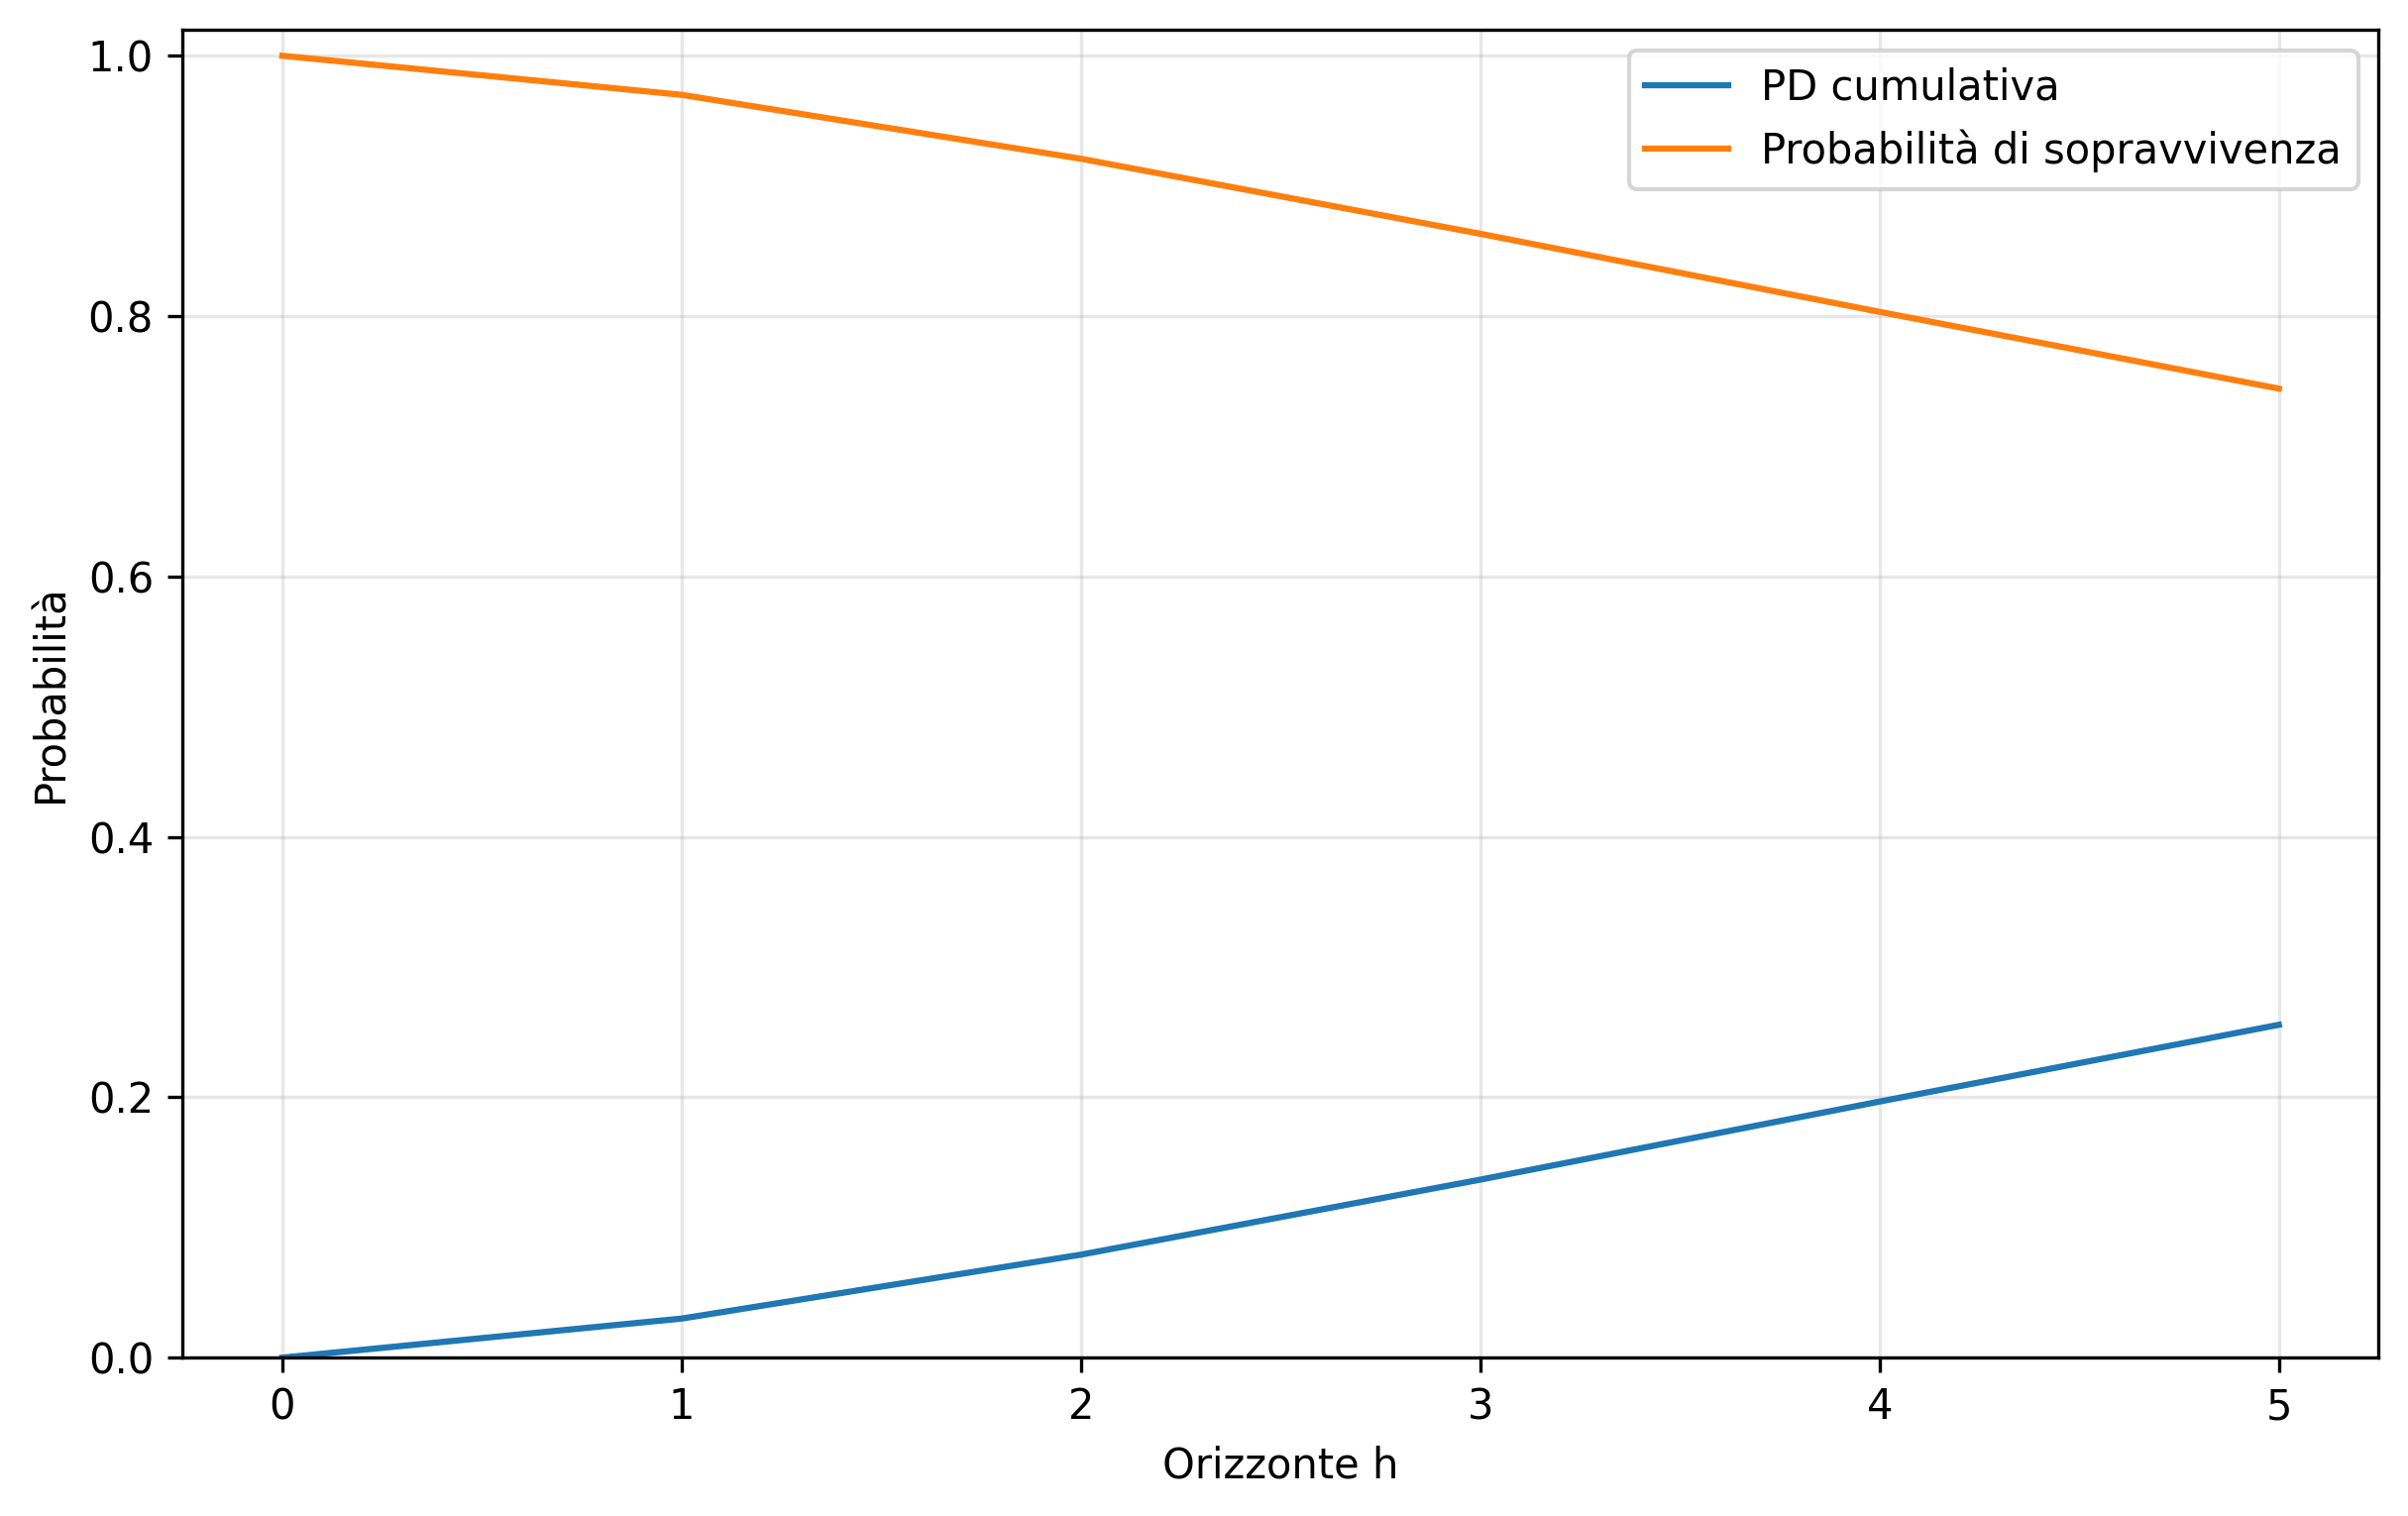
\includegraphics[width=0.78\textwidth]
{../graphics/Cap09_term_structure_default_esercizio.png}
\caption{Term structure della probabilit\`{a} cumulativa di default e
della probabilit\`{a} di sopravvivenza, condizionatamente al rating
iniziale $X_0=2$. Le due quantit\`{a} sono complementari a ogni
orizzonte.}
\label{fig:cap09-term-structure-default-esercizio}
\end{figure}

\item La probabilit\`{a} cumulativa di default cresce con l'orizzonte,
poich\'{e} incorpora tutti i possibili ingressi in default verificatisi
entro la data considerata. Simmetricamente, la probabilit\`{a} di
sopravvivenza diminuisce.

La probabilit\`{a} marginale misura invece il contributo del singolo
anno all'aumento della probabilit\`{a} cumulativa. Nel modello
considerato essa cresce nei primi quattro anni e si riduce lievemente
nel quinto.

La probabilit\`{a} condizionata di default aumenta dal $3\%$ del primo
anno a circa il $7.34\%$ del quinto anno. Il confronto con la
probabilit\`{a} marginale evidenzia l'effetto del condizionamento: il
rischio del singolo periodo viene misurato rispetto agli emittenti che
sono ancora sopravvissuti all'inizio del periodo stesso.

\end{enumerate}

\begin{exercise}[Distribuzione della perdita da migrazione]

\label{ex:cap09-distribuzione-perdita}

Si consideri un emittente inizialmente classificato nello stato
$X_0=2$. Dalla matrice di transizione dell'Esercizio precedente, la
distribuzione del rating dopo un anno \`{e}

\[
\begin{array}{c|cccc}
j & 1 & 2 & 3 & D\\
\hline
\Prob(X_1=j\mid X_0=2)
&
0.05
&
0.78
&
0.14
&
0.03
\end{array}
\]

Il valore di riferimento dell'esposizione alla data $h=1$ \`{e}

\[
V^{\mathrm{ref}}(h=1)=100.
\]

Ai quattro possibili rating futuri vengono associati i valori

\[
\begin{array}{c|cccc}
j & 1 & 2 & 3 & D\\
\hline
V_j(1)
&
104
&
100
&
90
&
45
\end{array}
\]

Si definisce la perdita a un anno mediante

\[
L_1=\ell(X_1,1),
\]

dove

\[
\ell(j,1)
=
V^{\mathrm{ref}}(1)-V_j(1).
\]

Condizionatamente al valore iniziale $X_0=2$:

\begin{enumerate}

\item Determinare la perdita associata a ciascun rating futuro.

\item Costruire la funzione di massa della variabile casuale $L_1$.

\item Determinare la funzione di ripartizione $F_{L_1}$.

\item Calcolare la perdita attesa.

\item Calcolare il momento secondo della perdita.

\item Calcolare la varianza e la deviazione standard.

\item Interpretare economicamente la distribuzione e i contributi dei
diversi stati alla perdita attesa.

\end{enumerate}

\end{exercise}

\noindent
\textbf{Soluzione.}

\begin{enumerate}

\item La funzione di perdita associa a ciascuno stato futuro la
differenza tra il valore di riferimento e il valore dell'esposizione
nello stato considerato:

\[
\ell(j,1)
=
V^{\mathrm{ref}}(1)-V_j(1).
\]

Si ottiene:

\[
\begin{array}{c|cccc}
j & 1 & 2 & 3 & D\\
\hline
V_j(1)
&
104
&
100
&
90
&
45
\\
\ell(j,1)
&
-4
&
0
&
10
&
55
\end{array}
\]

Pertanto,

\[
L_1
=
\begin{cases}
-4 & \text{se }X_1=1,\\
0  & \text{se }X_1=2,\\
10 & \text{se }X_1=3,\\
55 & \text{se }X_1=D.
\end{cases}
\]

La perdita negativa associata allo stato $1$ rappresenta un guadagno
rispetto al valore di riferimento: il miglioramento del rating
determina infatti un aumento del valore dell'esposizione.

\item La funzione di massa della perdita \`{e} ottenuta trasferendo le
probabilit\`{a} degli stati futuri sui corrispondenti valori di
perdita:

\[
\begin{array}{c|cccc}
\lambda
&
-4
&
0
&
10
&
55
\\
\hline
\Prob(L_1=\lambda\mid X_0=2)
&
0.05
&
0.78
&
0.14
&
0.03
\end{array}
\]

Le probabilit\`{a} sommano a uno:

\[
0.05+0.78+0.14+0.03=1.
\]

La Figura~\ref{fig:cap09-distribuzione-perdita-esercizio} rappresenta
la funzione di massa della perdita.

\begin{figure}[htbp]
\centering
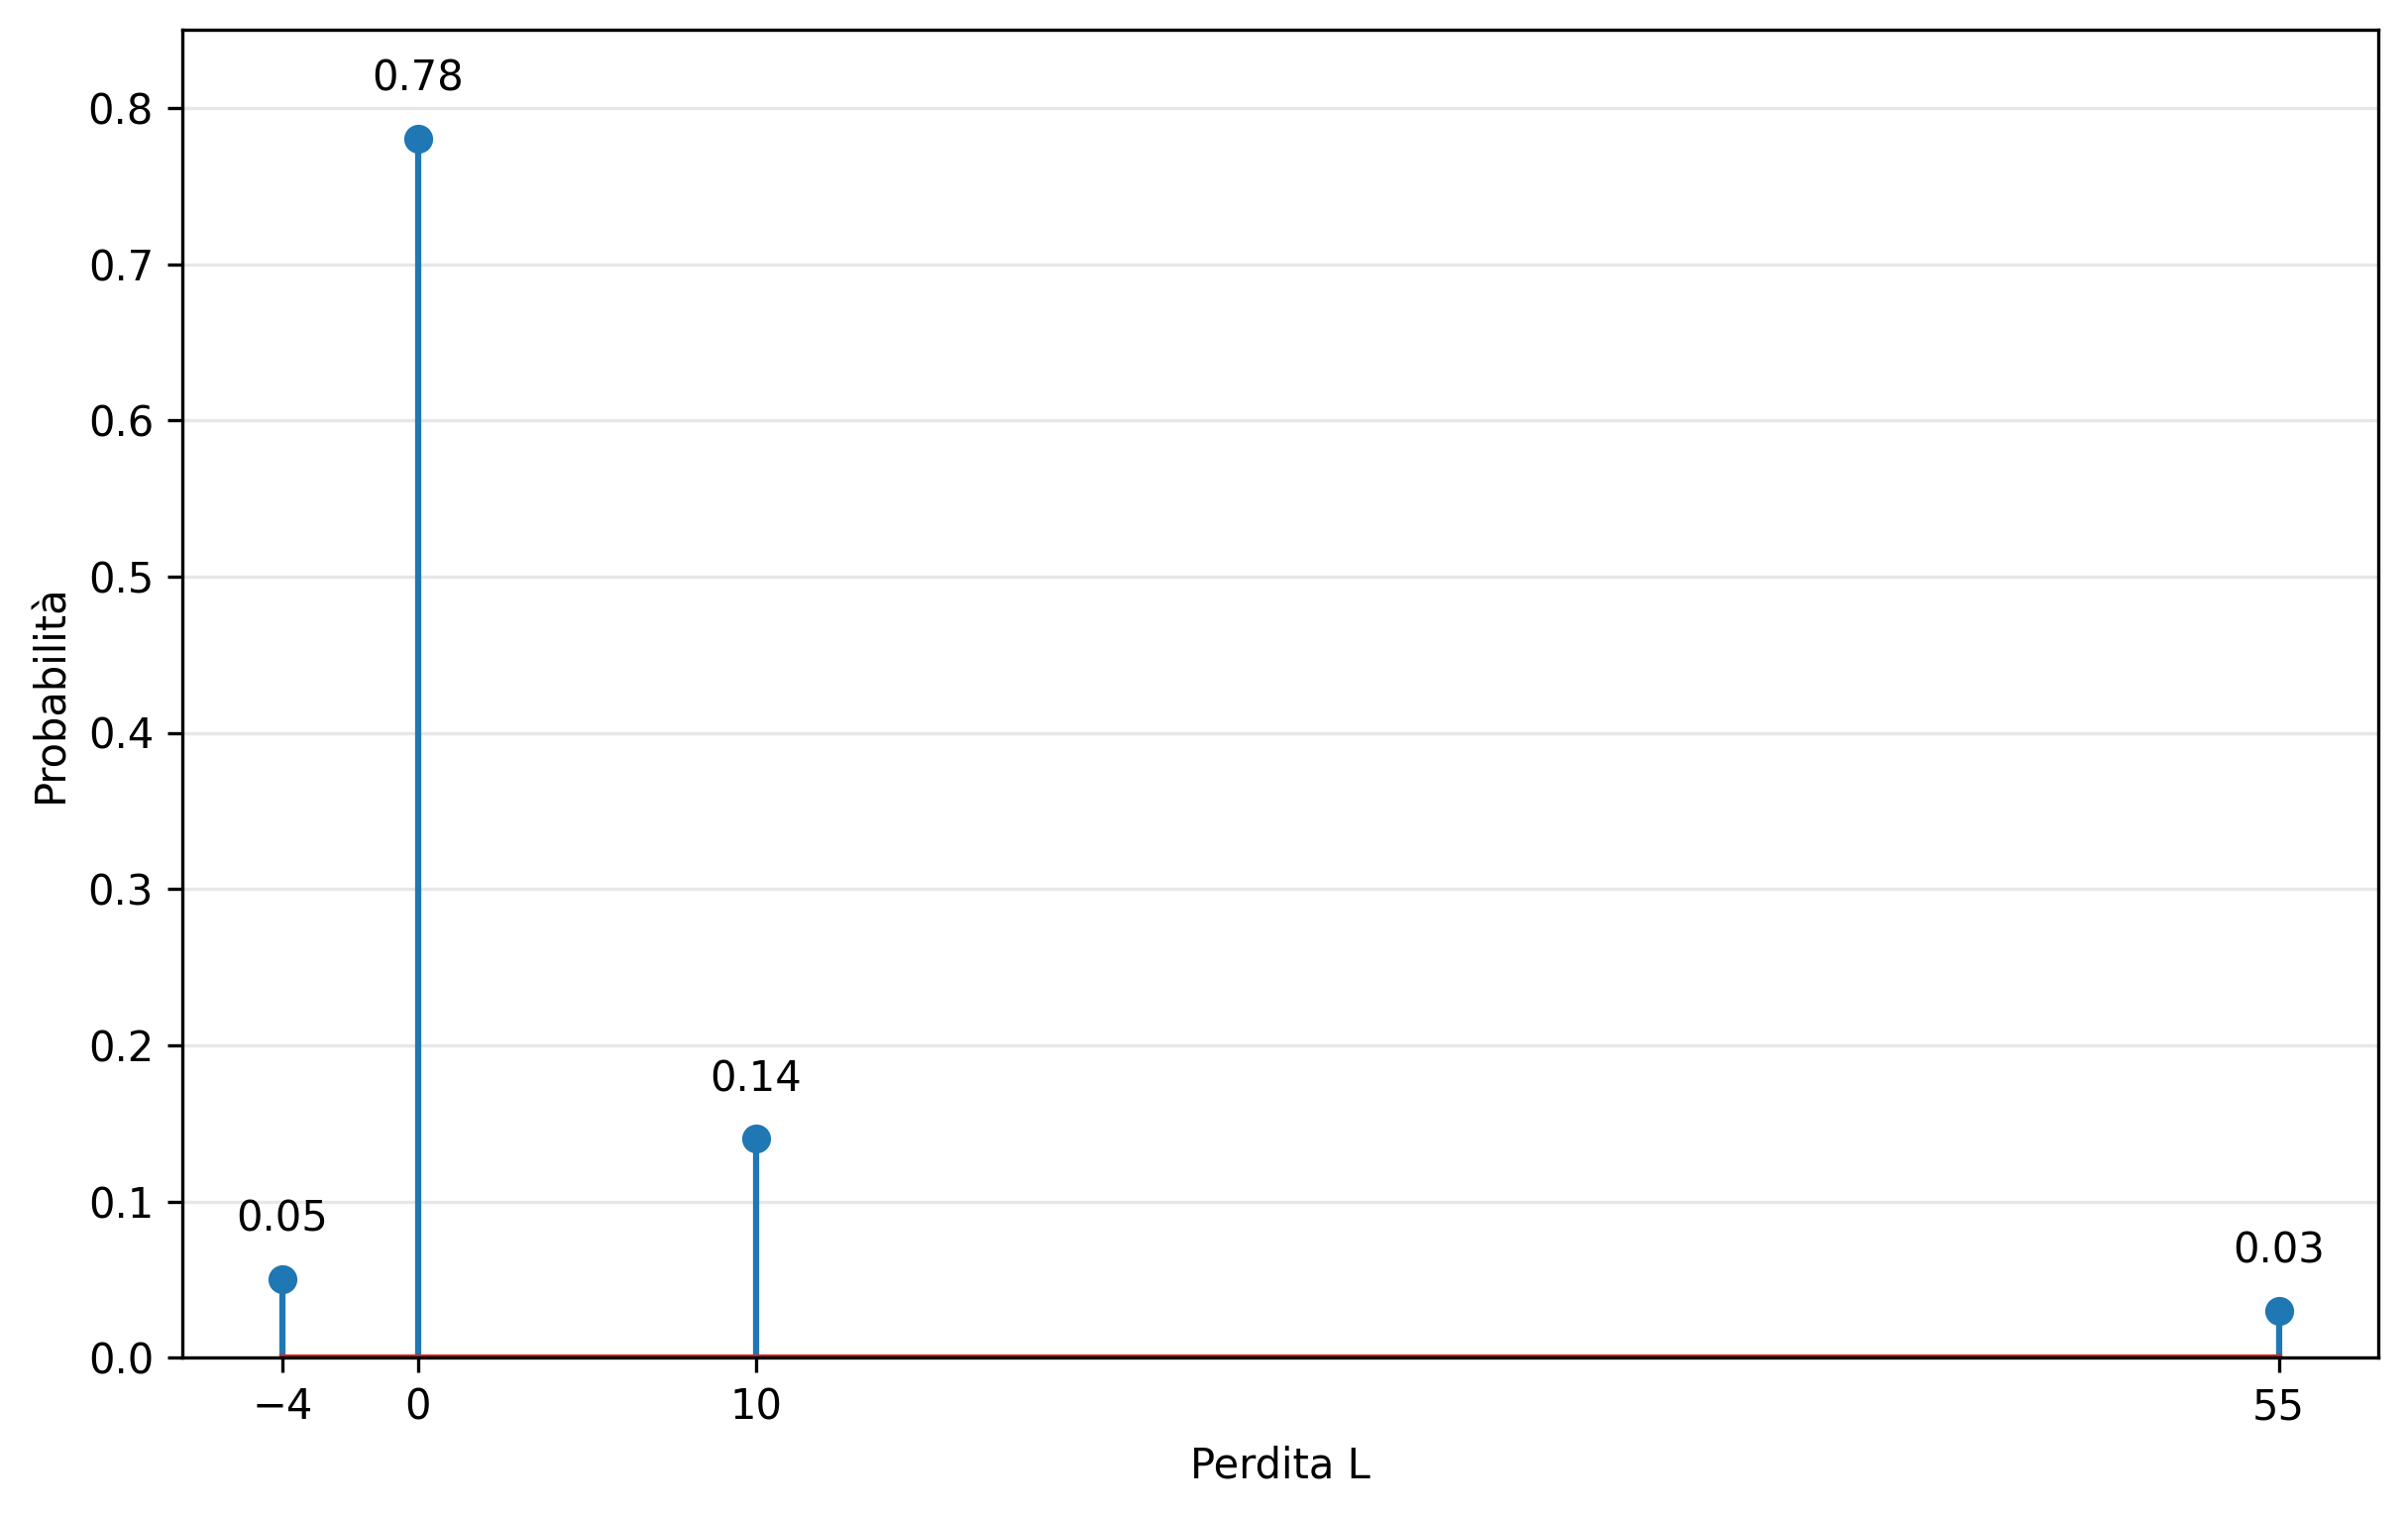
\includegraphics[width=0.78\textwidth]
{../graphics/Cap09_distribuzione_perdita_esercizio.png}
\caption{Funzione di massa della perdita a un anno associata alla
migrazione del rating. La maggior parte della probabilit\`{a} \`{e}
concentrata sulla perdita nulla, mentre il default genera una perdita
elevata ma poco probabile.}
\label{fig:cap09-distribuzione-perdita-esercizio}
\end{figure}

\item La funzione di ripartizione \`{e}

\[
F_{L_1}(\lambda)
=
\Prob(L_1\leq\lambda\mid X_0=2).
\]

Ordinando i possibili valori della perdita,

\[
-4<0<10<55,
\]

si ottiene:

\[
F_{L_1}(\lambda)
=
\begin{cases}
0
&
\text{se }\lambda<-4,
\\
0.05
&
\text{se }-4\leq\lambda<0,
\\
0.83
&
\text{se }0\leq\lambda<10,
\\
0.97
&
\text{se }10\leq\lambda<55,
\\
1
&
\text{se }\lambda\geq55.
\end{cases}
\]

In corrispondenza dei quattro valori della perdita:

\[
\begin{array}{c|cccc}
\lambda
&
-4
&
0
&
10
&
55
\\
\hline
F_{L_1}(\lambda)
&
0.05
&
0.83
&
0.97
&
1
\end{array}
\]

\item La perdita attesa, condizionatamente al rating iniziale, \`{e}

\[
\E^{\Prob}[L_1\mid X_0=2]
=
\sum_{j\in\mathcal{I}}
\ell(j,1)
\Prob(X_1=j\mid X_0=2).
\]

Sostituendo i valori:

\[
\begin{split}
\mathrm{EL}_2(1)
&=
(-4)(0.05)
+
(0)(0.78)
\\
&\quad
+
(10)(0.14)
+
(55)(0.03)
\\
&=
-0.20+0+1.40+1.65
\\
&=
2.85.
\end{split}
\]

Esplicitando i contributi economici:

\[
\begin{split}
\mathrm{EL}_2(1)
&=
\underbrace{(-4)(0.05)}_{\text{upgrade}}
+
\underbrace{(0)(0.78)}_{\text{permanenza}}
\\
&\quad
+
\underbrace{(10)(0.14)}_{\text{downgrade}}
+
\underbrace{(55)(0.03)}_{\text{default}}.
\end{split}
\]

La perdita attesa a un anno \`{e} quindi pari a

\[
\boxed{\mathrm{EL}_2(1)=2.85}.
\]

\item Il momento secondo \`{e}

\[
\E^{\Prob}[L_1^2\mid X_0=2]
=
\sum_{\lambda}
\lambda^2
\Prob(L_1=\lambda\mid X_0=2).
\]

Pertanto,

\[
\begin{split}
\E^{\Prob}[L_1^2\mid X_0=2]
&=
(-4)^2(0.05)
+
0^2(0.78)
\\
&\quad
+
10^2(0.14)
+
55^2(0.03)
\\
&=
16(0.05)
+
100(0.14)
+
3025(0.03)
\\
&=
0.80+14+90.75
\\
&=
105.55.
\end{split}
\]

\item La varianza si ottiene dalla relazione

\[
\Var(L_1\mid X_0=2)
=
\E^{\Prob}[L_1^2\mid X_0=2]
-
\left(
\E^{\Prob}[L_1\mid X_0=2]
\right)^2.
\]

Quindi,

\[
\begin{split}
\Var(L_1\mid X_0=2)
&=
105.55-(2.85)^2
\\
&=
105.55-8.1225
\\
&=
97.4275.
\end{split}
\]

La deviazione standard \`{e}

\[
\begin{split}
\sigma_{L_1}
&=
\sqrt{\Var(L_1\mid X_0=2)}
\\
&=
\sqrt{97.4275}
\\
&\approx
9.87.
\end{split}
\]

\item La distribuzione \`{e} fortemente asimmetrica. Con probabilit\`{a}

\[
0.05+0.78=0.83
\]

l'emittente migliora il proprio rating oppure rimane nella classe
iniziale, producendo una perdita non positiva. La probabilit\`{a} di
una perdita strettamente positiva \`{e} invece

\[
\Prob(L_1>0\mid X_0=2)
=
0.14+0.03
=
0.17.
\]

Il downgrade produce una perdita moderata pari a $10$, mentre il
default produce una perdita molto pi\`{u} elevata, pari a $55$.

Nonostante la probabilit\`{a} di default sia soltanto del $3\%$, il suo
contributo alla perdita attesa \`{e}

\[
55(0.03)=1.65,
\]

superiore al contributo del downgrade:

\[
10(0.14)=1.40.
\]

Il default domina ancora pi\`{u} nettamente il momento secondo:

\[
55^2(0.03)=90.75,
\]

su un valore complessivo pari a $105.55$. La dispersione della perdita
dipende quindi soprattutto dalla presenza di un evento raro ma di
grande severit\`{a}.

\end{enumerate}

\begin{exercise}[VaR e CVaR di una distribuzione discreta]

\label{ex:cap09-var-cvar-discreti}

Si riprenda la distribuzione della perdita a un anno costruita
nell'Esercizio~\ref{ex:cap09-distribuzione-perdita}:

\[
\begin{array}{c|cccc}
\lambda
&
-4
&
0
&
10
&
55
\\
\hline
\Prob(L_1=\lambda\mid X_0=2)
&
0.05
&
0.78
&
0.14
&
0.03
\end{array}
\]

Si consideri il livello di confidenza

\[
\alpha=0.95.
\]

\begin{enumerate}

\item Determinare il $\VaR_{0.95}(L_1)$.

\item Individuare la coda peggiore di probabilit\`{a} $1-\alpha=0.05$
e stabilire quale parte della massa collocata nel punto quantilico
deve essere inclusa nella coda.

\item Calcolare il $\CVaR_{0.95}(L_1)$ come media delle perdite
appartenenti alla coda peggiore del $5\%$.

\item Verificare il risultato mediante la rappresentazione

\[
\CVaR_{\alpha}(L)
=
\min_{\eta\in\R}
\left\{
\eta
+
\frac{1}{1-\alpha}
\E^{\Prob}
\left[
(L-\eta)^{+}
\right]
\right\}.
\]

\item Calcolare

\[
\E^{\Prob}
\left[
L_1
\mid
L_1\geq\VaR_{0.95}(L_1),\ X_0=2
\right]
\]

e spiegare perch\'{e} tale valore non coincide con il
$\CVaR_{0.95}(L_1)$.

\end{enumerate}

\end{exercise}

\noindent
\textbf{Soluzione.}

\begin{enumerate}

\item La funzione di ripartizione della perdita assume, nei punti del
supporto, i valori

\[
\begin{array}{c|cccc}
\lambda
&
-4
&
0
&
10
&
55
\\
\hline
F_{L_1}(\lambda)
&
0.05
&
0.83
&
0.97
&
1
\end{array}
\]

Per definizione,

\[
\VaR_{0.95}(L_1)
=
\inf
\left\{
\lambda\in\R:
F_{L_1}(\lambda)\geq0.95
\right\}.
\]

Poich\'{e}

\[
F_{L_1}(0)=0.83<0.95
\]

e

\[
F_{L_1}(10)=0.97\geq0.95,
\]

si ottiene

\[
\boxed{
\VaR_{0.95}(L_1)=10
}.
\]

Il VaR indica quindi che il quantile di livello $0.95$ della
distribuzione della perdita \`{e} pari a $10$.

\item La coda peggiore deve avere probabilit\`{a}

\[
1-\alpha=0.05.
\]

Le perdite strettamente superiori al VaR comprendono soltanto il valore

\[
L_1=55,
\]

che ha probabilit\`{a}

\[
\Prob(L_1>10\mid X_0=2)=0.03.
\]

Per completare la coda peggiore del $5\%$ occorre quindi includere
un'ulteriore probabilit\`{a}

\[
0.05-0.03=0.02
\]

proveniente dalla massa collocata nel punto quantilico

\[
L_1=10.
\]

La massa complessiva in tale punto \`{e}

\[
\Prob(L_1=10\mid X_0=2)=0.14.
\]

Nella coda entra pertanto soltanto la quota

\[
\frac{0.02}{0.14}
=
\frac{1}{7}
\]

della massa associata alla perdita $10$. La restante probabilit\`{a}

\[
0.14-0.02=0.12
\]

rimane fuori dalla coda peggiore selezionata.

La composizione della coda \`{e} quindi

\[
\begin{array}{c|cc}
\text{perdita}
&
10
&
55
\\
\hline
\text{massa inclusa nella coda}
&
0.02
&
0.03
\end{array}
\]

e le corrispondenti probabilit\`{a} normalizzate sono

\[
\frac{0.02}{0.05}=0.40,
\qquad
\frac{0.03}{0.05}=0.60.
\]

La Figura~\ref{fig:cap09-cvar-massa-quantile-esercizio} mostra la
selezione della coda peggiore del $5\%$.

\begin{figure}[htbp]
\centering
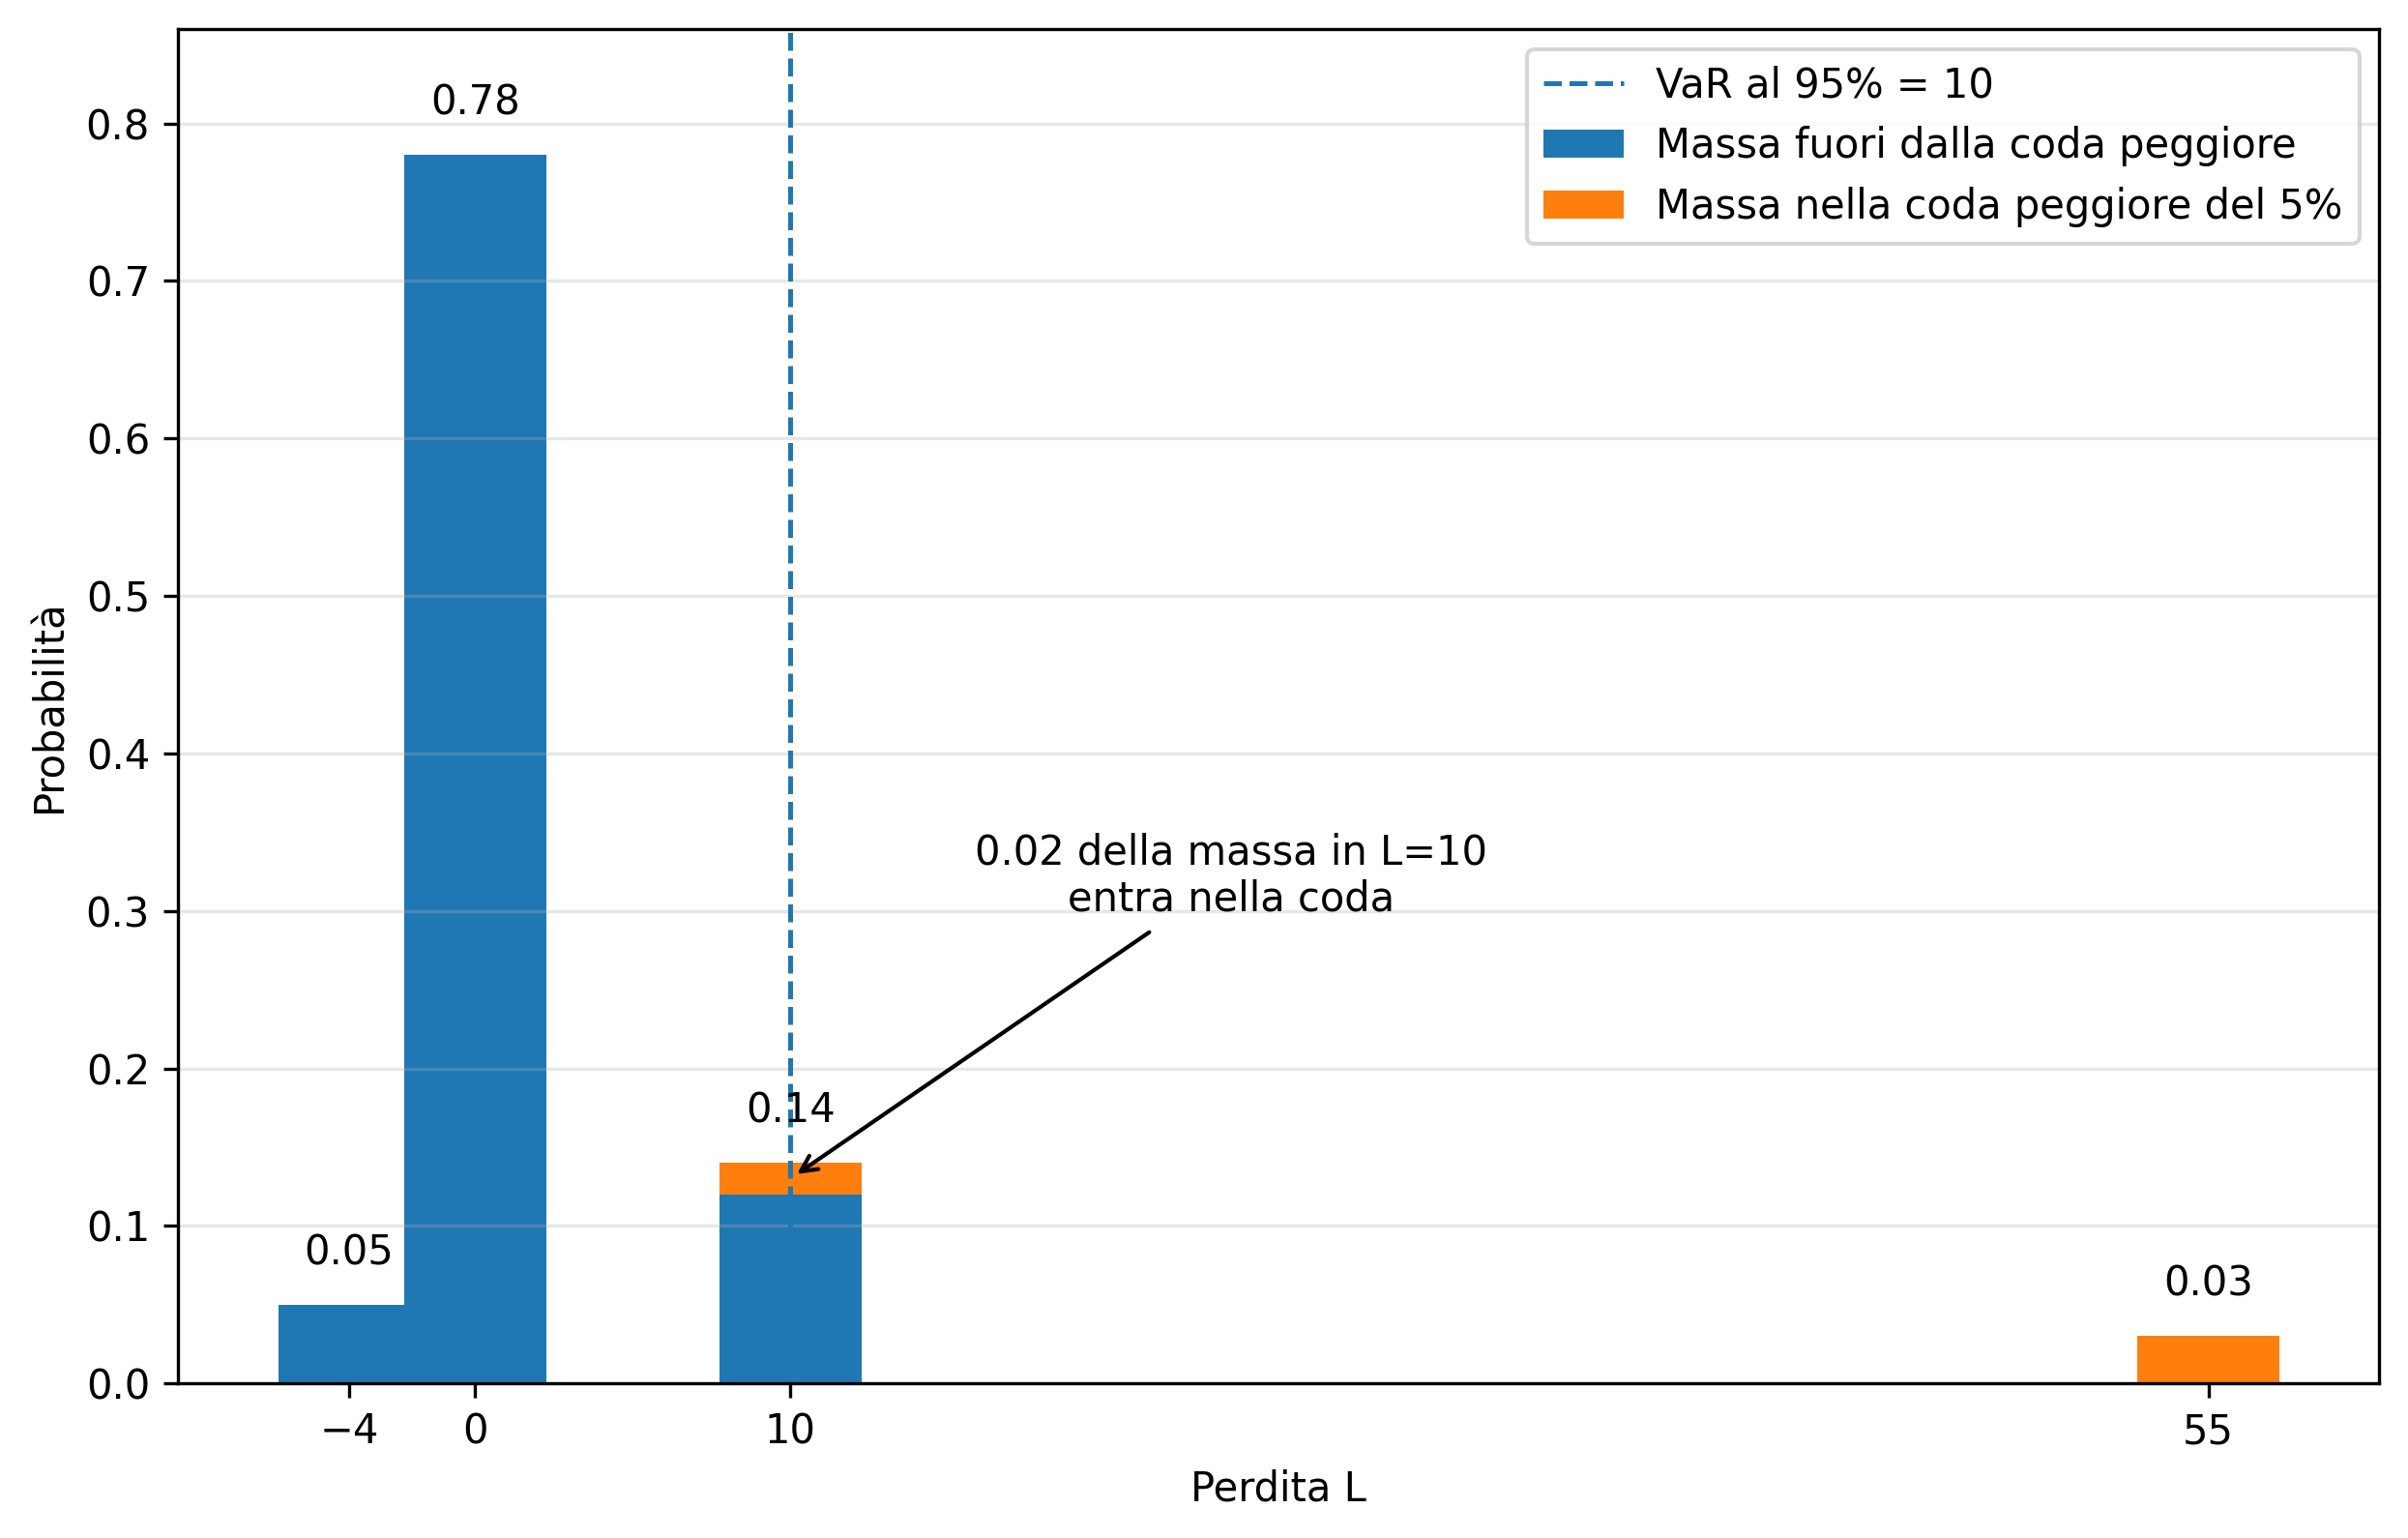
\includegraphics[width=0.82\textwidth]
{../graphics/Cap09_CVaR_massa_quantile_esercizio.png}
\caption{Composizione della coda peggiore del $5\%$. La coda comprende
tutta la massa associata alla perdita $55$ e soltanto una parte della
massa collocata nel punto quantilico $L_1=10$.}
\label{fig:cap09-cvar-massa-quantile-esercizio}
\end{figure}

\item Il CVaR \`{e} la media delle perdite appartenenti alla coda
peggiore, dopo avere normalizzato le masse rispetto alla probabilit\`{a}
complessiva della coda:

\[
\begin{split}
\CVaR_{0.95}(L_1)
&=
10
\frac{0.02}{0.05}
+
55
\frac{0.03}{0.05}
\\
&=
10(0.40)+55(0.60)
\\
&=
4+33
\\
&=
37.
\end{split}
\]

Pertanto,

\[
\boxed{
\CVaR_{0.95}(L_1)=37
}.
\]

Il CVaR \`{e} nettamente superiore al VaR:

\[
\CVaR_{0.95}(L_1)=37
>
10=\VaR_{0.95}(L_1),
\]

poich\'{e} incorpora anche la perdita estrema pari a $55$.

\item Nella rappresentazione basata sulla parte positiva, poniamo

\[
\eta=\VaR_{0.95}(L_1)=10.
\]

Si ha

\[
(L_1-10)^{+}
=
\begin{cases}
0 & \text{se }L_1=-4,\\
0 & \text{se }L_1=0,\\
0 & \text{se }L_1=10,\\
45 & \text{se }L_1=55.
\end{cases}
\]

Pertanto,

\[
\begin{split}
\E^{\Prob}
\left[
(L_1-10)^{+}
\mid X_0=2
\right]
&=
45(0.03)
\\
&=
1.35.
\end{split}
\]

Sostituendo nella formula:

\[
\begin{split}
\CVaR_{0.95}(L_1)
&=
10
+
\frac{1}{1-0.95}(1.35)
\\
&=
10+20(1.35)
\\
&=
10+27
\\
&=
37.
\end{split}
\]

Si ritrova quindi lo stesso risultato:

\[
\boxed{
\CVaR_{0.95}(L_1)=37
}.
\]

La massa parzialmente selezionata al quantile di livello $0.95$ non
compare esplicitamente nel termine

\[
\E^{\Prob}[(L_1-\eta)^{+}],
\]

poich\'{e} per $L_1=\eta=10$ la parte positiva \`{e} nulla. Il suo
effetto \`{e} incorporato nel termine iniziale $\eta$ della
rappresentazione.

\item L'evento

\[
\left\{
L_1\geq\VaR_{0.95}(L_1)
\right\}
\]

comprende tutta la massa associata alle perdite $10$ e $55$. La sua
probabilit\`{a} \`{e}

\[
\Prob(L_1\geq10\mid X_0=2)
=
0.14+0.03
=
0.17.
\]

Il corrispondente valore atteso condizionato \`{e}

\[
\begin{split}
\E^{\Prob}
\left[
L_1
\mid
L_1\geq10,\ X_0=2
\right]
&=
\frac{
10(0.14)+55(0.03)
}{
0.17
}
\\
&=
\frac{1.40+1.65}{0.17}
\\
&=
\frac{3.05}{0.17}
\\
&\approx
17.94.
\end{split}
\]

Si ottiene quindi

\[
\E^{\Prob}
\left[
L_1
\mid
L_1\geq\VaR_{0.95}(L_1),\ X_0=2
\right]
\approx
17.94,
\]

mentre

\[
\CVaR_{0.95}(L_1)=37.
\]

Le due quantit\`{a} non coincidono perch\'{e} l'evento

\[
\{L_1\geq10\}
\]

ha probabilit\`{a} $0.17$, mentre la coda richiesta per il calcolo del
CVaR deve avere probabilit\`{a} esattamente pari a $0.05$.

Il valore atteso condizionato include tutta la massa $0.14$ collocata
nel punto quantilico. Il CVaR include invece soltanto la quota $0.02$
necessaria a completare la coda peggiore del $5\%$.

In presenza di distribuzioni discrete, pertanto,

\[
\CVaR_{\alpha}(L)
\neq
\E^{\Prob}
\left[
L
\mid
L\geq\VaR_{\alpha}(L)
\right]
\]

in generale.

\end{enumerate}

\begin{exercise}[Sensibilit\`{a} dello spread equo di un CDS]

\label{ex:cap09-sensibilita-spread-cds}

Si consideri un CDS con nozionale

\[
N=100
\]

e scadenza $H=3$. I fattori di sconto sono

\[
d_1=0.98,
\qquad
d_2=0.95,
\qquad
d_3=0.92.
\]

Nel primo scenario, le probabilit\`{a} marginali risk-neutral di
default sono

\[
\Prob^{\Q}(\tau_D=1)=0.03,
\qquad
\Prob^{\Q}(\tau_D=2)=0.04,
\qquad
\Prob^{\Q}(\tau_D=3)=0.05.
\]

Le probabilit\`{a} di sopravvivenza sono pertanto

\[
\Prob^{\Q}(\tau_D>1)=0.97,
\qquad
\Prob^{\Q}(\tau_D>2)=0.93,
\qquad
\Prob^{\Q}(\tau_D>3)=0.88.
\]

Si assume che il premio alla data $h$ venga pagato soltanto se
$\tau_D>h$.

\begin{enumerate}

\item Con recovery rate $R=0.40$, calcolare il valore attuale della
gamba di protezione e il coefficiente della gamba dei premi.

\item Determinare lo spread equo $s^*$.

\item Ripetere il calcolo per $R=0.30$ e $R=0.50$, mantenendo
invariate le probabilit\`{a} risk-neutral.

\item Considerare un secondo scenario con probabilit\`{a} marginali
risk-neutral

\[
0.04,
\qquad
0.05,
\qquad
0.07.
\]

Calcolare il nuovo spread equo per $R=0.40$.

\item Interpretare separatamente l'effetto del recovery rate e quello
delle probabilit\`{a} risk-neutral.
\end{enumerate}
\end{exercise}

\noindent
\textbf{Soluzione.}

\begin{enumerate}

\item Introduciamo il fattore attualizzato associato alla gamba di
protezione:

\[
A_{\mathrm{prot}}
=
\sum_{h=1}^{3}
d_h
\Prob^{\Q}(\tau_D=h).
\]

Sostituendo i dati:

\[
\begin{split}
A_{\mathrm{prot}}
&=
(0.98)(0.03)
+
(0.95)(0.04)
+
(0.92)(0.05)
\\
&=
0.0294+0.0380+0.0460
\\
&=
0.1134.
\end{split}
\]

Il valore attuale della gamba di protezione, per $R=0.40$, \`{e}

\[
\begin{split}
\mathrm{PV}_{\mathrm{prot}}
&=
N(1-R)A_{\mathrm{prot}}
\\
&=
100(0.60)(0.1134)
\\
&=
6.804.
\end{split}
\]

Per la gamba dei premi definiamo

\[
A_{\mathrm{prem}}
=
\sum_{h=1}^{3}
d_h
\Prob^{\Q}(\tau_D>h).
\]

Si ottiene:

\[
\begin{split}
A_{\mathrm{prem}}
&=
(0.98)(0.97)
+
(0.95)(0.93)
+
(0.92)(0.88)
\\
&=
0.9506+0.8835+0.8096
\\
&=
2.6437.
\end{split}
\]

Pertanto,

\[
\mathrm{PV}_{\mathrm{prem}}(s)
=
sNA_{\mathrm{prem}}
=
264.37s.
\]

\item Lo spread equo $s^{*}$ rende uguali i valori attuali delle due
gambe:

\[
\mathrm{PV}_{\mathrm{prot}}
=
\mathrm{PV}_{\mathrm{prem}}(s^{*}).
\]

Quindi,

\[
6.804
=
264.37s^{*},
\]

da cui

\[
s^{*}
=
\frac{6.804}{264.37}
\approx
0.02574.
\]

Lo spread equo annuale \`{e} quindi circa

\[
\boxed{
s^{*}=2.574\%
}
\]

ossia

\[
\boxed{
s^{*}\approx257.4\text{ punti base}.
}
\]

Il nozionale compare in entrambe le gambe e si semplifica nella
determinazione dello spread:

\[
s^{*}
=
(1-R)
\frac{
A_{\mathrm{prot}}
}{
A_{\mathrm{prem}}
}.
\]

\begin{figure}[htbp]
\centering
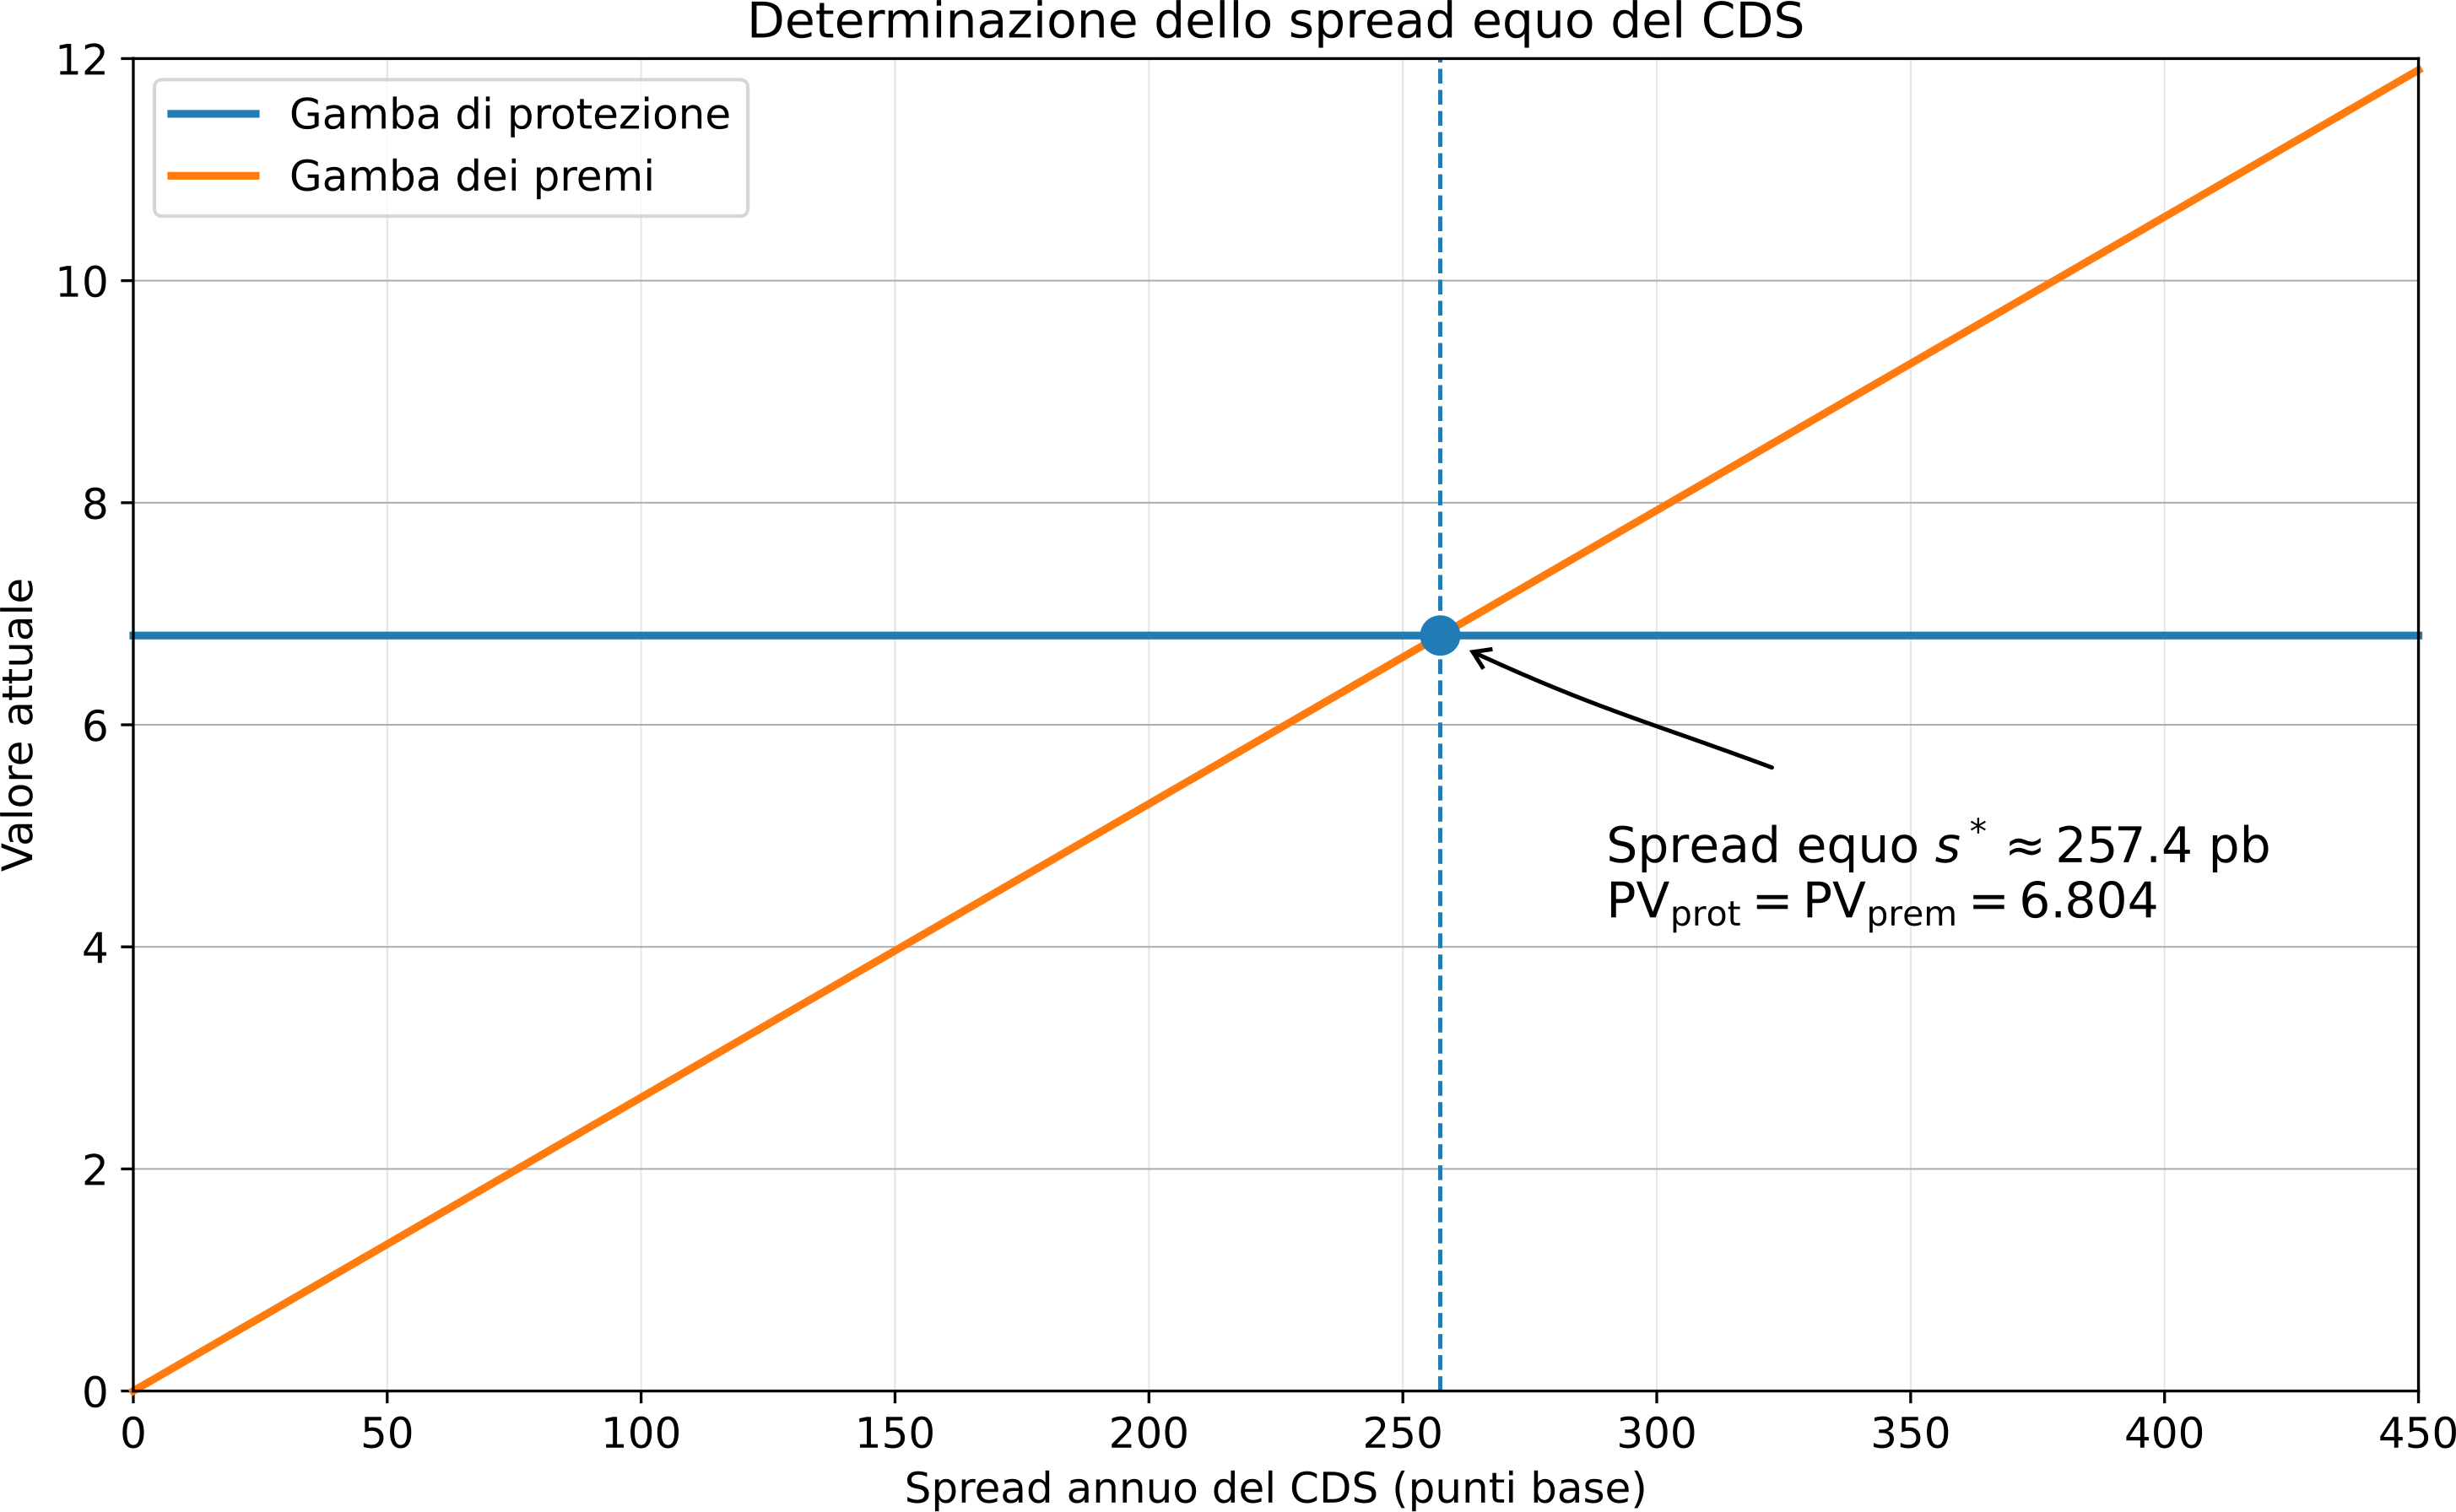
\includegraphics[width=0.90\textwidth]
{../graphics/Cap09_CDS_equilibrio_gambe.png}
\caption{Determinazione dello spread equo del CDS. Il valore attuale
della gamba di protezione non dipende dallo spread contrattuale,
mentre il valore attuale della gamba dei premi cresce linearmente con
esso. Il punto di intersezione identifica lo spread equo
$s^{*}\approx257.4$ punti base, per il quale le due gambe hanno valore
attuale pari a $6.804$.}
\label{fig:cap09-cds-equilibrio-gambe}
\end{figure}

\item Mantenendo invariate le probabilit\`{a} risk-neutral e i fattori
di sconto, la sensibilit\`{a} rispetto al recovery rate \`{e}

\[
s^{*}(R)
=
(1-R)
\frac{0.1134}{2.6437}.
\]

Per $R=0.30$:

\[
\begin{split}
s^{*}(0.30)
&=
0.70
\frac{0.1134}{2.6437}
\\
&\approx
0.03003,
\end{split}
\]

ossia circa

\[
\boxed{
300.3\text{ punti base}.
}
\]

Per $R=0.50$:

\[
\begin{split}
s^{*}(0.50)
&=
0.50
\frac{0.1134}{2.6437}
\\
&\approx
0.02145,
\end{split}
\]

ossia circa

\[
\boxed{
214.5\text{ punti base}.
}
\]

A parit\`{a} delle altre condizioni, un recovery rate pi\`{u} elevato
riduce il pagamento atteso della protezione e quindi riduce lo spread
equo.

\item Nel secondo scenario, le probabilit\`{a} marginali risk-neutral
di default sono

\[
0.04,
\qquad
0.05,
\qquad
0.07.
\]

Le corrispondenti probabilit\`{a} di sopravvivenza sono:

\[
\Prob^{\Q}(\tau_D>1)=0.96,
\]

\[
\Prob^{\Q}(\tau_D>2)
=
1-0.04-0.05
=
0.91,
\]

e

\[
\Prob^{\Q}(\tau_D>3)
=
1-0.04-0.05-0.07
=
0.84.
\]

Il nuovo fattore della gamba di protezione \`{e}

\[
\begin{split}
A_{\mathrm{prot}}^{(2)}
&=
(0.98)(0.04)
+
(0.95)(0.05)
+
(0.92)(0.07)
\\
&=
0.0392+0.0475+0.0644
\\
&=
0.1511.
\end{split}
\]

Il fattore della gamba dei premi \`{e}

\[
\begin{split}
A_{\mathrm{prem}}^{(2)}
&=
(0.98)(0.96)
+
(0.95)(0.91)
+
(0.92)(0.84)
\\
&=
0.9408+0.8645+0.7728
\\
&=
2.5781.
\end{split}
\]

Con $R=0.40$:

\[
\begin{split}
s^{*}_{2}
&=
0.60
\frac{0.1511}{2.5781}
\\
&\approx
0.03517.
\end{split}
\]

Il nuovo spread equo \`{e} quindi

\[
\boxed{
s^{*}_{2}\approx351.7\text{ punti base}.
}
\]

\item Il recovery rate incide sulla severit\`{a} del pagamento di
protezione:

\[
N(1-R).
\]

Mantenendo fisse le probabilit\`{a} risk-neutral, una riduzione di $R$
aumenta quindi lo spread equo.

Un aumento delle probabilit\`{a} risk-neutral di default produce invece
due effetti:

\begin{itemize}

\item aumenta il valore attuale della gamba di protezione;

\item riduce le probabilit\`{a} di sopravvivenza e quindi il valore della
gamba dei premi per ogni unit\`{a} di spread.

\end{itemize}

Entrambi gli effetti determinano un aumento dello spread equo. I
confronti precedenti sono esercizi di sensibilit\`{a} parziale: ogni
parametro viene modificato mantenendo invariati gli altri dati del
modello.

\end{enumerate}

\section{Esercizi proposti}

\label{sec:cap09-esercizi-proposti}

Gli esercizi seguenti riprendono le principali componenti della catena
di misurazione sviluppata nel capitolo. Le applicazioni procedono dal
confronto tra differenti rappresentazioni della perdita creditizia
alla misurazione del rischio di portafoglio e agli scenari di stress.

\begin{exercise}[Modello default-only e modello migration-based]

\label{ex:cap09-default-only-migration-based}

Si considerino due emittenti, $A$ e $B$, inizialmente appartenenti alla
classe di rating $2$. Dopo un anno, le rispettive distribuzioni dei
rating sono:

\[
\begin{array}{c|cccc}
&
1
&
2
&
3
&
D
\\
\hline
A
&
0.08
&
0.75
&
0.14
&
0.03
\\
B
&
0.02
&
0.70
&
0.25
&
0.03
\end{array}
\]

I valori della perdita associati ai quattro stati sono:

\[
\begin{array}{c|cccc}
j
&
1
&
2
&
3
&
D
\\
\hline
\ell(j,1)
&
-3
&
0
&
8
&
60
\end{array}
\]

Nel modello \emph{default-only} si considera soltanto la perdita da
default:

\[
L^{\mathrm{DO}}
=
60\cdot\1_{\{X_1=D\}}.
\]

Nel modello \emph{migration-based} si considera invece

\[
L^{\mathrm{MB}}
=
\ell(X_1,1).
\]

\begin{enumerate}

\item Calcolare, per ciascun emittente, la perdita attesa e la varianza
nel modello \emph{default-only}.

\item Calcolare, per ciascun emittente, la perdita attesa e la varianza
nel modello \emph{migration-based}.

\item Confrontare i risultati ottenuti per gli emittenti $A$ e $B$.

\item Spiegare perch\'{e} la stessa probabilit\`{a} di default non
determina la stessa distribuzione della perdita.

\end{enumerate}

\textit{Risultati:} nel modello \emph{default-only}, per entrambi gli
emittenti,

\[
\mathrm{EL}^{\mathrm{DO}}=1.80,
\qquad
\Var(L^{\mathrm{DO}})=104.76.
\]

Nel modello \emph{migration-based},

\[
\mathrm{EL}^{\mathrm{MB}}_A=2.68,
\qquad
\Var(L_A^{\mathrm{MB}})=110.4976,
\]

mentre

\[
\mathrm{EL}^{\mathrm{MB}}_B=3.74,
\qquad
\Var(L_B^{\mathrm{MB}})=110.1924.
\]

\end{exercise}

\begin{exercise}[Stesso VaR e diverso CVaR]

\label{ex:cap09-stesso-var-diverso-cvar}

Si considerino le due distribuzioni discrete di perdita:

\[
\begin{array}{c|cccc}
\lambda
&
0
&
10
&
20
&
100
\\
\hline
\Prob(L_A=\lambda)
&
0.90
&
0.05
&
0.04
&
0.01
\\
\Prob(L_B=\lambda)
&
0.90
&
0.05
&
0.01
&
0.04
\end{array}
\]

\begin{enumerate}

\item Costruire le funzioni di ripartizione di $L_A$ e $L_B$.

\item Calcolare il VaR al livello di confidenza del $95\%$ per entrambe
le distribuzioni.

\item Calcolare il CVaR al livello di confidenza del $95\%$.

\item Confrontare le due misure e spiegare quale caratteristica della
distribuzione non viene rilevata dal VaR.

\end{enumerate}

\textit{Risultati:}

\[
\VaR_{0.95}(L_A)
=
\VaR_{0.95}(L_B)
=
10,
\]

mentre

\[
\CVaR_{0.95}(L_A)=36,
\qquad
\CVaR_{0.95}(L_B)=84.
\]

Le due distribuzioni hanno lo stesso quantile di livello $0.95$, ma
assegnano probabilit\`{a} molto differenti alla perdita estrema pari
a $100$.

\end{exercise}

\begin{exercise}[Orizzonte temporale e scenario di stress]

\label{ex:cap09-orizzonte-stress}

Si consideri una catena di rating con stati

\[
\mathcal{I}
=
\{
1=\text{qualit\`{a} elevata},
\,
2=\text{qualit\`{a} intermedia},
\,
D=\text{default}
\}.
\]

Nello scenario ordinario, la matrice annuale di transizione \`{e}

\[
P_{\mathrm{ord}}
=
\begin{pmatrix}
0.90&0.08&0.02\\
0.10&0.80&0.10\\
0&0&1
\end{pmatrix}.
\]

In uno scenario di stress viene invece utilizzata la matrice

\[
P_{\mathrm{stress}}
=
\begin{pmatrix}
0.82&0.12&0.06\\
0.05&0.70&0.25\\
0&0&1
\end{pmatrix}.
\]

L'emittente si trova inizialmente nello stato $X_0=2$.

\begin{enumerate}

\item Calcolare $P_{\mathrm{ord}}^2$, $P_{\mathrm{ord}}^3$,
$P_{\mathrm{stress}}^2$ e $P_{\mathrm{stress}}^3$.

\item Determinare le probabilit\`{a} cumulative di default a uno, due
e tre anni nei due scenari.

\item Calcolare le corrispondenti probabilit\`{a} marginali di default
e le probabilit\`{a} di sopravvivenza.

\item Confrontare l'effetto congiunto dell'allungamento dell'orizzonte
e della sostituzione della matrice ordinaria con quella di stress.

\end{enumerate}

\textit{Risultati:} nello scenario ordinario,

\[
\begin{array}{c|ccc}
h
&
1
&
2
&
3
\\
\hline
\mathrm{PD}^{\mathrm{cum}}_2(h)
&
0.1000
&
0.1820
&
0.2502
\\
\mathrm{PD}^{\mathrm{marg}}_2(h)
&
0.1000
&
0.0820
&
0.0682
\\
S_2(h)
&
0.9000
&
0.8180
&
0.7498
\end{array}
\]

Nello scenario di stress,

\[
\begin{array}{c|ccc}
h
&
1
&
2
&
3
\\
\hline
\mathrm{PD}^{\mathrm{cum}}_2(h)
&
0.2500
&
0.4280
&
0.5566
\\
\mathrm{PD}^{\mathrm{marg}}_2(h)
&
0.2500
&
0.1780
&
0.1286
\\
S_2(h)
&
0.7500
&
0.5720
&
0.4434
\end{array}
\]

\end{exercise}

\begin{exercise}[Posizione coperta e posizione non coperta]

\label{ex:cap09-copertura-cds}

La perdita di una posizione creditizia non coperta presenta la
distribuzione:

\[
\begin{array}{c|cccc}
\text{stato}
&
1
&
2
&
3
&
D
\\
\hline
\Prob(X_1=j)
&
0.10
&
0.72
&
0.14
&
0.04
\\
L^{\mathrm{unhedged}}
&
-2
&
0
&
12
&
50
\end{array}
\]

Un CDS paga $50$ in caso di default e nulla negli altri stati. Il
valore attuale equivalente dei premi \`{e} pari a $2.5$ ed \`{e}
trattato, in questo modello semplificato, come un costo certo.

La perdita coperta \`{e} quindi

\[
L^{\mathrm{hedged}}
=
L^{\mathrm{unhedged}}
-
50\cdot\1_{\{X_1=D\}}
+
2.5.
\]

\begin{enumerate}

\item Costruire la distribuzione della perdita coperta.

\item Calcolare la perdita attesa, il VaR al $95\%$ e il CVaR al
$95\%$ della posizione non coperta.

\item Calcolare le stesse misure per la posizione coperta.

\item Spiegare perch\'{e} la copertura pu\`{o} ridurre il CVaR senza
ridurre necessariamente la perdita attesa o il VaR.

\end{enumerate}

\textit{Risultati:} per la posizione non coperta,

\[
\mathrm{EL}^{\mathrm{unhedged}}=3.48,
\qquad
\VaR_{0.95}(L^{\mathrm{unhedged}})=12,
\]

\[
\CVaR_{0.95}(L^{\mathrm{unhedged}})=42.4.
\]

La distribuzione della posizione coperta \`{e}

\[
\begin{array}{c|ccc}
\lambda
&
0.5
&
2.5
&
14.5
\\
\hline
\Prob(L^{\mathrm{hedged}}=\lambda)
&
0.10
&
0.76
&
0.14
\end{array}
\]

e

\[
\mathrm{EL}^{\mathrm{hedged}}=3.98,
\qquad
\VaR_{0.95}(L^{\mathrm{hedged}})=14.5,
\]

\[
\CVaR_{0.95}(L^{\mathrm{hedged}})=14.5.
\]

\end{exercise}

\begin{exercise}[Dipendenza tra due esposizioni]

\label{ex:cap09-portafoglio-dipendenza}

Un portafoglio contiene due esposizioni. In caso di default del primo
emittente si verifica una perdita pari a $40$; in caso di default del
secondo emittente si verifica una perdita pari a $60$.

Le due probabilit\`{a} individuali di default sono

\[
\Prob(X_{1,h}=D)
=
\Prob(X_{2,h}=D)
=
0.05.
\]

Si confrontino due modelli:

\begin{itemize}

\item default indipendenti;

\item dipendenza positiva perfetta, per la quale i due emittenti
entrano sempre in default congiuntamente.

\end{itemize}

La perdita di portafoglio \`{e}

\[
L_h^{\mathrm{port}}
=
40\1_{\{X_{1,h}=D\}}
+
60\1_{\{X_{2,h}=D\}}.
\]

\begin{enumerate}

\item Costruire la distribuzione congiunta dei due indicatori di
default nei due modelli.

\item Determinare la distribuzione della perdita aggregata.

\item Calcolare la perdita attesa nei due casi.

\item Calcolare il VaR e il CVaR al livello di confidenza del $95\%$.

\item Spiegare perch\'{e} la perdita attesa rimane invariata, mentre
le misure di coda cambiano sensibilmente.

\end{enumerate}

\textit{Risultati:} sotto indipendenza,

\[
\begin{array}{c|cccc}
\lambda
&
0
&
40
&
60
&
100
\\
\hline
\Prob(L_h^{\mathrm{port}}=\lambda)
&
0.9025
&
0.0475
&
0.0475
&
0.0025
\end{array}
\]

e

\[
\E^{\Prob}[L_h^{\mathrm{port}}]=5,
\qquad
\VaR_{0.95}(L_h^{\mathrm{port}})=40,
\]

\[
\CVaR_{0.95}(L_h^{\mathrm{port}})=62.
\]

Sotto dipendenza positiva perfetta,

\[
\begin{array}{c|cc}
\lambda
&
0
&
100
\\
\hline
\Prob(L_h^{\mathrm{port}}=\lambda)
&
0.95
&
0.05
\end{array}
\]

e

\[
\E^{\Prob}[L_h^{\mathrm{port}}]=5,
\qquad
\VaR_{0.95}(L_h^{\mathrm{port}})=0,
\]

\[
\CVaR_{0.95}(L_h^{\mathrm{port}})=100.
\]

\end{exercise}

\section{Sintesi e raccordo con la Lezione 10}

\label{sec:cap09-sintesi-raccordo}

Il capitolo ha sviluppato il passaggio dalle probabilit\`{a} di
transizione tra rating alla distribuzione monetaria delle perdite
creditizie. La costruzione richiede di collegare tre componenti:
l'evoluzione probabilistica degli stati, le conseguenze economiche
associate a ciascuno stato futuro e le misure utilizzate per descrivere
la distribuzione della perdita.

La sequenza concettuale complessiva pu\`{o} essere sintetizzata come
segue:

\[
\boxed{
\begin{array}{c}
\text{PD marginali, cumulative e sopravvivenza}
\\[2mm]
\downarrow
\\[2mm]
\text{PD, LGD, EAD e valori associati ai rating}
\\[2mm]
\downarrow
\\[2mm]
\text{distribuzione della perdita}
\\[2mm]
\downarrow
\\[2mm]
\text{\emph{Expected Loss}, \emph{VaR} e \emph{CVaR}}
\\[2mm]
\downarrow
\\[2mm]
P^{\Prob}\ \text{per il rischio}
\qquad
P^{\Q}\ \text{per il pricing}
\\[2mm]
\downarrow
\\[2mm]
\text{CDS e copertura}
\\[2mm]
\downarrow
\\[2mm]
\text{portafoglio, dipendenza e simulazione}
\end{array}
}
\]

Le potenze della matrice di transizione permettono anzitutto di
determinare la struttura temporale del default. La probabilit\`{a}
cumulativa misura il rischio di default entro un dato orizzonte; la
probabilit\`{a} marginale isola il contributo del singolo periodo; la
probabilit\`{a} di sopravvivenza descrive la permanenza negli stati
non-default.

Queste probabilit\`{a} non determinano, da sole, una distribuzione
monetaria. Occorre associare a ciascuno stato futuro una conseguenza
economica. Nel modello default-only la perdita dipende essenzialmente
da \emph{Exposure at Default} (\emph{EAD}) e \emph{Loss Given Default}
(\emph{LGD}); nel modello basato sulle migrazioni del rating assume
rilievo anche la variazione del valore dell'esposizione negli stati
non-default.

La funzione di perdita realizza tale passaggio:

\[
L_h=\ell(X_h,h),
\qquad
\ell(j,h)=V^{\mathrm{ref}}(h)-V_j(h).
\]

Una volta costruita la distribuzione di $L_h$, la
\emph{Expected Loss} (\emph{EL}) ne misura il valore medio, mentre il
\emph{Value at Risk} (\emph{VaR}) e il \emph{Conditional Value at
Risk} (\emph{CVaR}) descrivono la parte superiore della distribuzione.
Il VaR individua un quantile della perdita; il CVaR considera anche la
severit\`{a} degli esiti appartenenti alla coda peggiore. Nel caso di
distribuzioni discrete, il suo calcolo pu\`{o} richiedere l'inclusione
parziale della massa associata al valore del VaR.

La distinzione tra misura fisica e misura risk-neutral separa due
finalit\`{a} differenti. Le probabilit\`{a} sotto $\Prob$ vengono
utilizzate per prevedere le perdite e misurare il rischio. Le
probabilit\`{a} sotto $\Q$ vengono invece utilizzate per valutare i
flussi finanziari coerentemente con i prezzi di mercato.

Nel caso del \emph{Credit Default Swap} (\emph{CDS}), il premio equo
rende uguali il valore attuale della gamba dei premi e quello della
gamba di protezione. La copertura modifica la distribuzione della
perdita, ma non elimina necessariamente tutte le sue componenti. Il
costo dei premi, le perdite da downgrade, il rischio di controparte e
il \emph{basis risk} possono produrre una posizione residua ancora
esposta al rischio creditizio.

Il passaggio dalla singola esposizione al portafoglio introduce infine
la dipendenza tra i debitori. La perdita aggregata

\[
L_h^{\mathrm{port}}
=
\sum_{n=1}^{N}L_{n,h}
\]

dipende non soltanto dalle distribuzioni individuali, ma anche dalla
probabilit\`{a} che downgrade e default si verifichino congiuntamente.
Concentrazione, fattori macroeconomici comuni e rischio sistematico
assumono quindi un ruolo essenziale nella determinazione delle perdite
estreme.

La Lezione~10 svilupper\`{a} operativamente questo ultimo passaggio.
Per portafogli con molte esposizioni, il numero delle possibili
configurazioni dei rating cresce rapidamente e rende poco praticabile
la costruzione analitica della distribuzione congiunta. La simulazione
permette invece di generare un numero elevato di scenari e di
ricostruire empiricamente la distribuzione della perdita aggregata.

In ciascuna replica della simulazione si proceder\`{a} a:

\begin{enumerate}

\item generare gli eventuali fattori economici comuni;

\item simulare le transizioni dei singoli emittenti, condizionatamente
ai rating iniziali e ai fattori comuni;

\item associare a ciascuno stato futuro la corrispondente perdita e
aggregare le perdite individuali;

\item ripetere la procedura per stimare la distribuzione della perdita
di portafoglio, la perdita attesa e le misure di rischio di coda.

\end{enumerate}

Il raccordo tra le due lezioni pu\`{o} quindi essere sintetizzato come
segue:

\[
\boxed{
\begin{array}{c}
\text{Lezione 9}
\\
\text{costruzione teorica della distribuzione della perdita}
\\[2mm]
\downarrow
\\[2mm]
\text{Lezione 10}
\\
\text{simulazione della distribuzione di portafoglio}
\\[2mm]
\downarrow
\\[2mm]
\text{stima empirica di EL, VaR e CVaR}
\end{array}
}
\]

